% !TeX spellcheck = en_GB
 
\newglossaryentry{pseudoinverse}
{name={pseudoinverse},
  description={The \index{pseudoinverse}Moore–Penrose pseudoinverse $\mA^{+}$ 
 	of a matrix $\mA \in \mathbb{R}^{\samplesize \times \nrfeatures}$ generalizes the 
 	notion of an \gls{inverse} \cite{GolubVanLoanBook}. The pseudoinverse arises naturally 
 	within \gls{ridgeregression} when applied to a \gls{dataset} with arbitrary \glspl{label} $\vy$ 
 	and a \gls{featuremtx} $\mX = \mA$ \cite[Ch.\ 3]{hastie01statisticallearning}. The \gls{modelparams} 
 	learned by \gls{ridgeregression} 
  	are given by
  	\[
  	\widehat{\vw}^{(\regparam)}  = \big(\mA^T \mA + \regparam \mI \big)^{-1} \mA^\top \vy, \quad \regparam > 0.
  	\]
  	We can then define the pseudoinverse  $\mA^+ \in \mathbb{R}^{\nrfeatures \times \samplesize}$ via 
  	the limit \cite[Ch. 3]{benisrael2003generalized}
  	\[
  	\lim_{\regparam \to 0^+} \widehat{\vw}^{(\regparam)} = \mA^+ \vy.
  	\]
	\\
	See also: \gls{inverse}, \gls{ridgeregression}, \gls{dataset}, \gls{label}, \gls{featuremtx}, \gls{modelparams}, \gls{ridgeregression}.
	},
 first={pseudoinverse},
 text={pseudoinverse}
}

\newglossaryentry{inverse}
{name={inverse matrix},
 description={An inverse matrix\index{inverse matrix} $\mA^{-1}$ is defined for a 
 	square matrix $\mA \in \mathbb{R}^{n \times n}$ that is of full rank, meaning its 
 	columns are linearly independent. In this case, $\mA$ is said to be invertible, 
 	and its inverse satisfies 
 	\[
 	\mA \mA^{-1} = \mA^{-1} \mA = \mI.
 	\]  	
     	A square matrix is invertible if and only if its \gls{det} is non-zero. Inverse matrices are 
     	fundamental in solving systems of linear equations and in the closed-form solution of 
     	\gls{linreg} \cite{Strang2007}, \cite{Horn91}.  The concept of an inverse matrix can be extended 
     	to matrices that are not square or not full rank. One may define a ``left inverse'' $\mB$ 
     	satisfying $\mB \mA = \mI$, or a ``right inverse'' $\mC$ satisfying $\mA \mC = \mI$. 
     	For general rectangular or singular matrices, the Moore–Penrose \gls{pseudoinverse}
     	$\mA^{+}$ provides a unified concept of generalized inverse matrix \cite{GolubVanLoanBook}.
 	 \begin{figure}[H]
 		\centering
 		\begin{tikzpicture}[x=2cm,y=2cm]
 			% LEFT: Standard basis
 			\begin{scope}
 				\draw[->, thick] (0,0) -- (1,0) node[below right] {$\vx$};
 				\draw[->, thick] (0,0) -- (0,1) node[above left] {$\vy$};
 			\end{scope}
 			% CENTER: Transformed basis (by A)
 			\begin{scope}[shift={(2.0,0)}]
 				\coordinate (A) at (1.5,0.5);
 				\coordinate (B) at (-0.2,1.2);
				\draw[->, very thick, red] (0,0) -- (A) node[pos=0.5, below right] {$\mA \vx$};
 				\draw[->, very thick, red] (0,0) -- (B) node[above right] {$\mA \vy$};
 			\end{scope}
 			% RIGHT: Inverse transformation
 			\begin{scope}[shift={(4.9,0)}]
 				\draw[->, very thick, blue] (0,0) -- (1,0) node[pos=0.5, below] {$\mA^{-1} (\mA \vx) = \vx$};
 				\draw[->, very thick, blue] (0,0) -- (0,1) node[above] {$\mA^{-1} (\mA \vy) = \vy$};
 			\end{scope}
 			% Curved arrows between stages
 			\draw[->, thick, bend left=20] (1.2,0.4) to node[above] {$\mA$} (1.8,0.4);
 			\draw[->, thick, bend left=20] (3.8,0.4) to node[below] {$\mA^{-1}$} (4.4,0.4);
 		\end{tikzpicture}
 		\caption{A matrix $\mathbf{A}$ represents a linear transformation of $\mathbb{R}^{2}$. The inverse matrix $\mathbf{A}^{-1}$ 
 			represents the inverse transformation. \label{fig_matrix_inverse_dict}} 
 		\end{figure}
		See also: \gls{det}, \gls{linreg}, \gls{pseudoinverse}.},
	first={inverse matrix},
	text={inverse matrix}
}

\newglossaryentry{det}
{name={determinant},
	description={The\index{determinant} determinant $\det(\mA)$ of a square matrix 
	$\mA = \big( \va^{(1)},\ldots, \va^{(n)} \big) \in \mathbb{R}^{n \times n}$ is a 
	function of its columns $\va^{(1)},\ldots,\va^{(n)} \in \mathbb{R}^{n}$ that is \cite{DirschmidHansJorg1996TuF}
	\begin{itemize}
		\item normalized: $$\det (\mI) = 1,$$ 
		\item multi-linear: \begin{align} \nonumber \det \big(\va^{(1)},\ldots,\alpha\vu+ \beta \vv,\ldots,\va^{(n)} \big) & = \alpha\det \big(\va^{(1)},\ldots,\vu,\ldots,\va^{(n)} \big) \\ 
			& +\beta\det \big(\va^{(1)},\ldots,\vv,\ldots,\va^{(n)} \big), \nonumber
			\end{align}
		\item anti-symmetric: $$\det \big(\ldots,\va^{(i)}, \ldots, \va^{(j)},\ldots \big) = - \det \big(\ldots,\va^{(j)}, \ldots, \va^{(i)},\ldots \big).$$ 
	\end{itemize} 
	We can interpret a matrix $\mA$ as a linear transformation on $\mathbb{R}^{n}$. 
	The determinant $\det(\mA)$ characterizes how (the orientation of) 
 	volumes in $\mathbb{R}^n$ are altered by this transformation \cite{GolubVanLoanBook}, \cite{Strang2007}. 
 	In particular, $\det(\mA) > 0$ preserves orientation, $\det(\mA) < 0$ reverses orientation, 
 	and $\det(\mA) = 0$ collapses volume entirely, indicating that $\mA$ is non-invertible. 
 	The determinant also satisfies $\det(\mA \mB) = \det(\mA) \cdot \det(\mB)$, and if $\mA$ is 
 	diagonalizable with \glspl{eigenvalue} $\eigval{1}, \ldots, \eigval{n}$, then $\det(\mA) = \prod_{i=1}^{n} \eigval{i}$ \cite{HornMatAnalysis}.
    	For the special cases $n=2$ (2D) and $n=3$ (3D), the determinant can be interpreted as an oriented 
    	area or volume spanned by the column vectors of $\mA$.
    	\begin{figure}[H]
    	\begin{center}
    	\begin{tikzpicture}[x=2cm]
	% LEFT: Standard basis vectors and unit square
	\begin{scope}
	\draw[->, thick] (0,0) -- (1,0) node[below right] {$\vx$};
	\draw[->, thick] (0,0) -- (0,1) node[above left] {$\vy$};
	%\draw[fill=gray!15] (0,0) -- (1,0) -- (1,1) -- (0,1) -- cycle;
	%\node at (0.5,0.5) {\small unit square};
	%\node at (0.5,-0.6) {standard basis};
	\end{scope}
	% RIGHT: Transformed basis vectors and parallelogram
	\begin{scope}[shift={(2.8,0)}]
	\coordinate (A) at (1.5,0.5);
	\coordinate (B) at (-0.2,1.2);
	\draw[->, very thick, red] (0,0) -- (A) node[below right] {$\mA \vx$};
	\draw[->, very thick, red] (0,0) -- (B) node[above left] {$\mA \vy$};
	\draw[fill=red!20, opacity=0.6] (0,0) -- (A) -- ($(A)+(B)$) -- (B) -- cycle;
	\draw[dashed] (A) -- ($(A)+(B)$);
	\draw[dashed] (B) -- ($(A)+(B)$);
	\node at (0.8,0.6) {\small $\det(\mA)$};
	% Orientation arc
	\draw[->, thick, blue] (0.4,0.0) arc[start angle=0, end angle=35, radius=0.6];
	%	\node[blue] at (0.25,1.25) {};
	%	\node at (0.8,-0.6) {transformed basis};
	\end{scope}
	% Arrow between plots
	\draw[->, thick] (1.3,0.5) -- (2.4,0.5) node[midway, above] {$\mA$};
	\end{tikzpicture}
	\end{center}
	\end{figure}
		See also: \gls{eigenvalue}, \gls{inverse}.},
	first={determinant},
	text={determinant}
}

\newglossaryentry{linearmap}
{name={linear map}, plural={linear maps}, 
	description={A\index{linear map} linear \gls{map} $f: \mathbb{R}^n \rightarrow \mathbb{R}^m$ is a \gls{function} that satisfies additivity, i.e.,
		$f(\vx + \vy) = f(\vx) + f(\vy)$, and homogeneity, i.e.,
		$f(c\vx) = c f(\vx)$, for all vectors $\vx, \vy \in \mathbb{R}^n$ and scalars $c \in \mathbb{R}$. 
		In particular, $f(\mathbf{0}) = \mathbf{0}$. Any linear \gls{map} can be represented as a matrix 
		multiplication $f(\vx) = \mA \vx$ for some matrix $\mA \in \mathbb{R}^{m \times n}$. 
		The collection of real-valued linear \glspl{map} for a given dimension $n$ constitute a \gls{linmodel} 
		which is used in many \gls{ml} methods.\\
		See also: \gls{map}, \gls{function}, \gls{linmodel}, \gls{ml}.},
	first={linear map},
	text={linear map}
}


\newglossaryentry{vectorspace}
{name={vector space},
	description={A\index{vector space} vector space (also called linear space) is a collection of elements (called vectors) closed under vector addition and scalar multiplication, i.e.,
		\begin{itemize}
			\item If $\vx, \vy \in \mathcal{V}$, then $\vx + \vy \in \mathcal{V}$.
			\item If $\vx \in \mathcal{V}$ and $c \in \mathbb{R}$, then $c \vx \in \mathcal{V}$.
			\item In particular, $\mathbf{0} \in \mathcal{V}$.
		\end{itemize}
		The \gls{euclidspace} $\mathbb{R}^n$ is a vector space.
		\Glspl{linmodel} and \glspl{linearmap} operate within such spaces.\\
		See also: \gls{euclidspace}, \gls{linmodel}, \gls{linearmap}.},
	first={vector space},
	text={vector space}
}


\newglossaryentry{stochastic}
{name={stochastic},
	description={We refer to a \index{stochastic} method as stochastic if it involves a random component 
		or is governed by probabilistic laws. \Gls{ml} methods use randomness to reducing 
		computational complexity (see, e.g., \gls{stochGD}) or to capture \gls{uncertainty} in \glspl{probmodel}. 
	 \\
		See also: \gls{uncertainty}, \gls{probmodel}, \gls{stochGD}.},
	first={stochastic},
	text={stochastic}
}

\newglossaryentry{stochproc}
{name={stochastic process},
	description={A stochastic process is a collection of \glspl{rv} defined over a common \gls{probspace}. 
		These \glspl{rv} are indexed by time or space, which are used to model random phenomena
		evolving over time (e.g., noise in sensors or financial time series). Random \glspl{graph}, 
		such as \gls{sbm} or \gls{ergraph}, are another example of stochastic processes. These processes 
		use pairs of nodes in a \gls{graph} as the index set. We can also use stochastic processes 
		to represent \glspl{stochalgorithm} such as \gls{stochGD}. 
		\\
		See also:  \gls{stochGD}, \gls{uncertainty}, \gls{probmodel}, \gls{rv}, \gls{sbm}.},
	first={stochastic process},
	text={stochastic process}
}


\newglossaryentry{characteristicfunc}
{name={characteristic function},
	description={The characteristic function\index{characteristic function} 
		of a real-valued \gls{rv} $x$ is the function \cite[Section 26]{BillingsleyProbMeasure}
		$$ \phi_{x}(t) \defeq \expect { \exp(j t x) } \mbox{ with } j = \sqrt{-1}.$$
	 The characteristic function uniquely determines the \gls{probdist} of $x$. 
		\\
		See also: \gls{probdist}, \gls{rv}.},
	first={characteristic function},
	firstplural={characteristic functions}, 
	plural={characteristic functions},
	text={characteristic function}
}




\newglossaryentry{entropy}
{name={entropy},
  description={Entropy quantifies the \gls{uncertainty} or unpredictability associated with a \gls{rv} \cite{coverthomas}. 
		  For a discrete \gls{rv} $x$ taking values in a finite set $\mathcal{S} = \{x_1, \ldots, x_n\}$ with 
		probability mass function $p_i \defeq \prob{x = x_i}$, the entropy is defined as
		\[
		H(x) \defeq -\sum_{i=1}^n p_i \log p_i.
		\]
		Entropy is maximized when all outcomes are equally likely, and minimized (i.e., zero) 
		when the outcome is deterministic. A generalization of the concept of entropy for continuous 
		\glspl{rv} is \gls{diffentropy}. 
\\
		See also: \gls{uncertainty}, \gls{probmodel}.},
	first={entropy},
	text={entropy}
}

\newglossaryentry{diffentropy}
{name={differential entropy},
	description={For\index{differential entropy} a real-valued \gls{rv} $\featurevec \in \mathbb{R}^{\nrfeatures}$ 
		with \gls{pdf} $p(x)$,
		the differential entropy is defined as \cite{coverthomas}
		\[
		h(\featurevec) \defeq - \int p(\featurevec) \log p(\featurevec) \, d\featurevec.
		\]
		Differential entropy can be negative and lacks some properties of \gls{entropy} for 
		discrete-valued \glspl{rv}, such as invariance under change of variables \cite{coverthomas}. 
		Among all \glspl{rv} with given \gls{mean} $\meanvecgeneric$ and \gls{covmtx} $\covmtxgeneric$, 
		$h(\featurevec)$ is maximized by $\featurevec \sim \mvnormal{\meanvecgeneric}{\covmtxgeneric}$. 
		\\
		See also: \gls{uncertainty}, \gls{probmodel}.},
	first={differential entropy},
	text={differential entropy}
}


\newglossaryentry{minimum}
{name=minimum,
	description={Given a set of real numbers, the minimum\index{minimum} is the smallest of those numbers.
		Note that for some sets, such as the set of negative real numbers, the minimum does not exist.},
	firstplural={minima}, 
 	plural={minima},
	first={minimum},
	text={minimum}
}

\newglossaryentry{function}
{name={function}, plural={functions}, 
	description={A function\index{function} is a relation between two sets $\mathcal{U}$ and $\mathcal{V}$ such that for each  
	element of the first set $u \in \mathcal{U}$ there is associated exactly one element of the second set $v \in \mathcal{V}$ 
	\cite{RudinBookPrinciplesMatheAnalysis}. 
		  We write this as $f: \mathcal{U} \rightarrow \mathcal{V}$, where $\mathcal{U}$ is the domain 
		  and $\mathcal{V}$ the co-domain of $f$. That is, a function $f$ defines a unique 
		  output $f(u) \in \mathcal{V}$ for every input $u \in \mathcal{U}$. 
	},
	first={function},
	text={function}
}


\newglossaryentry{map}
{name={map}, plural={maps}, 
	description={We\index{map} use the term map as a synonym for \gls{function}.
	\\
	See also: \gls{function}.},
	first={map},
	text={map}
}


\newglossaryentry{optproblem}
{name={optimization problem}, 
	description={An\index{optimization problem} optimization problem is a mathematical 
		   structure consisting of an \gls{objfunc} $f: \mathcal{U} \rightarrow \mathcal{V}$ 
		   defined over an optimization variable $\weights \in \mathcal{U}$, together with a 
		   feasible set $\mathcal{W} \subseteq \mathcal{U}$. The co-domain $\mathcal{V}$ is 
		   assumed to be ordered, meaning that for any two elements $\mathbf{a}, \mathbf{b} \in \mathcal{V}$, 
		   we can determine whether $\mathbf{a} < \mathbf{b}$, $\mathbf{a} = \mathbf{b}$, 
		   or $\mathbf{a} > \mathbf{b}$. The goal of optimization is to find those values $\weights \in \mathcal{W}$ 
		   for which the objective $f(\weights)$ is extremal—i.e., minimal or maximal \cite{BoydConvexBook}, \cite{nesterov04}, \cite{BertsekasNonLinProgr}.
		   \\
		   See also: \gls{objfunc}.},
	first={optimization problem},
	firstplural={optimization problems}, 
	plural={optimization problems}, 
	text={optimization problem}
}

\newglossaryentry{optmethod}
{name={optimization method},
	description={An\index{optimization method} optimization method is an \gls{algorithm} that 
		reads in a representation of an \gls{optproblem} and delivers an (approximate) solution 
		as its output \cite{BoydConvexBook}, \cite{nesterov04}, \cite{BertsekasNonLinProgr}.
		 \\
		 See also: \gls{algorithm}, \gls{optproblem}.},
	first={optimization method},
	firstplural={optimization methods}, 
	plural={optimization methods}, 
	text={optimization method}
}

\newglossaryentry{fixedpointiter}
{name={fixed-point iteration},
	description={A\index{fixed-point iteration} fixed-point iteration is an iterative method for solving 
		a given \gls{optproblem}. It constructs a sequence $\weights^{(0)}, \weights^{(1)},\ldots$ by 
		 repeatedly applying an operator $\fixedpointop$, i.e., 
		 \begin{equation} 
		 	\label{equ_def_fixed_point_dict} 
		 	\weights^{(\iteridx+1)} = \fixedpointop \weights^{(\iteridx)} \mbox{, for } \iteridx=0,1,\ldots.
		 \end{equation} 
		 The operator $\fixedpointop$ is chosen such that any of its fixed points is a solution 
		 $\widehat{\weights}$ to the given \gls{optproblem}. For example, given a \gls{differentiable} and 
		 \gls{convex} \gls{function} $f(\weights)$, the fixed points of the operator $\fixedpointop: \weights \mapsto \weights - \nabla f(\weights)$ 
		 coincide with the minimizers of $f(\weights)$. In general, for a given \gls{optproblem} with solution $\widehat{\weights}$, 
		 there are many different operators $\fixedpointop$ whose fixed points are $\widehat{\weights}$. 
		 Clearly, we should use an operator $\fixedpointop$ in \eqref{equ_def_fixed_point_dict} that reduces the distance to a solution such that
		 \begin{equation} 
			\nonumber
			\underbrace{\normgeneric{ \weights^{(\iteridx+1)} - \widehat{\netparams}}{2}}_{\stackrel{\eqref{equ_def_fixed_point_dict}}{=} \normgeneric{ \fixedpointop \weights^{(\iteridx)} - \fixedpointop\widehat{\weights}}{2}}  \leq 	\normgeneric{ \weights^{(\iteridx)} - \widehat{\weights}}{2}. 
		\end{equation}
		Thus, we require $\fixedpointop$ to be at least non-expansive, i.e., the iteration \eqref{equ_def_fixed_point_dict} 
		should not result in worse \gls{modelparams} that have a larger distance to a solution $\widehat{\weights}$. 
		What is more, each iteration \eqref{equ_def_fixed_point_dict} should also make some progress, i.e., 
		reduce the distance to a solution $\widehat{\weights}$. This requirement can be made precise using 
		the notion of a \gls{contractop} \cite{Bauschke:2017}, \cite{fixedpoinIsta}. 
		The operator $\fixedpointop$ is a \gls{contractop} if, for some $\contractfac \in [0,1)$,
		\begin{equation} 
			\nonumber
			\normgeneric{ \fixedpointop \weights\!-\!\fixedpointop \weights'}{2}  \leq  \contractfac	\normgeneric{\weights\!-\!\weights'}{2} \mbox{ holds for any } \weights,\weights'.
		\end{equation}
		For a \gls{contractop} $\fixedpointop$, the fixed-point iteration \eqref{equ_def_fixed_point_dict} generates 
		a sequence $\weights^{(\iteridx)}$ that converges quite rapidly. In particular \cite[Th. 9.23]{RudinBookPrinciplesMatheAnalysis}, 
		\begin{equation} 
			\nonumber
			\normgeneric{ \weights^{(\iteridx)} - \widehat{\weights}}{2} \leq \contractfac^{\iteridx} 	\normgeneric{ \weights^{(0)} - \widehat{\weights}}{2}. 
		\end{equation} 
		Here, $\normgeneric{ \weights^{(0)} - \widehat{\weights}}{2}$ is the distance between 
		the initialization $\weights^{(0)}$ and the solution $\widehat{\weights}$. 
		It turns out that a fixed-point iteration \eqref{equ_def_fixed_point_dict} with a firmly non-expansive 
		operator $\fixedpointop$ is guaranteed to converge to a fixed-point of $\fixedpointop$ \cite[Cor. 5.16]{Bauschke:2017}. 
		Figure \ref{fig_examples_nonexp_dict} depicts examples of a firmly non-expansive operator, a non-expansive operator, 
		and a \gls{contractop}. All these operators are defined on the one-dimensional space $\mathbb{R}$. 
		Another example of a firmly non-expansive operator is the \gls{proxop} of a \gls{convex} \gls{function} \cite{Bauschke:2017}, \cite{ProximalMethods}. 
		\definecolor{darkgreen}{rgb}{0.0, 0.5, 0.0}
		\begin{figure}[H]
			\begin{center} 
				\begin{tikzpicture}[scale=1.5]
					% Axes
					\draw[line width=1pt, ->] (-2,0) -- (2,0) node[right] {$\weight^{(\iteridx)}$};
					\draw[line width=1pt, ->] (0,-2) -- (0,2) node[above] {$\weight^{(\iteridx+1)}$};
					% Labels
					\node at (2.1,2.2) {$\fixedpointop^{(3)}$};
					\node at (1.9,-1.5) {$\fixedpointop^{(1)}$};
					\node at (1.5,1.2) {$\fixedpointop^{(2)}$};
					% Dashed lines at x=1 and y=1
					\draw[dashed] (1,-2) -- (1,2); % Vertical line at x=1
					\draw[dashed] (-2,1) -- (2,1); % Horizontal line at y=1
					\draw[dashed] (-2,-1) -- (2,-1); % Horizontal line at y=1
					\draw[dashed] (-1,-2) -- (-1,2); % Vertical line at x=1
					\node[above,xshift=4pt,yshift=-1pt] at (1,0) {$1$};
					\node[above,xshift=8pt,yshift=-1pt] at (0,-1) {$-1$};
					% First curve: y = 1/2 x + 1
					\draw[line width=2,domain=-2:2,smooth,blue] plot(\x,{0.5*\x + 1});
					% Second curve: y = -x
					\draw[line width=2,domain=-2:2,smooth,red] plot(\x,{-\x});
					% Third curve: y = x / |x| * min(|x|, 1)
					\draw[line width=2, domain=-2:-1,smooth,darkgreen] plot(\x,{-1});
					\draw[line width=2,domain=-1:1,smooth,darkgreen] plot(\x,{\x});
					\draw[line width=2,domain=1:2,smooth,darkgreen] plot(\x,{1});
				\end{tikzpicture}
			\end{center} 
			\caption{Example of a non-expansive operator $\fixedpointop^{(1)}$, a firmly non-expansive operator $\fixedpointop^{(2)}$, and 
				a \gls{contractop} $\fixedpointop^{(3)}$. \label{fig_examples_nonexp_dict}}
		\end{figure} 
		See also: \gls{optproblem}, \gls{differentiable}, \gls{convex} \gls{function}, \gls{modelparams}, \gls{contractop}, \gls{proxop}.},
	first={fixed-point iteration},
	text={fixed-point iteration},
	firstplural={fixed-point iterations}, 
	plural={fixed-point iterations}
}


\newglossaryentry{ergraph}
{name={Erd\H{o}s-R\'enyi graph (ER graph)},
	description={An ER  \gls{graph} is a \gls{probmodel} for \glspl{graph} defined over 
		a given node set $\nodeidx=1,\ldots,\nrnodes$. One way to define the ER \gls{graph} is 
		via the collection of \gls{iid} binary \glspl{rv} $b^{(\edge{\nodeidx}{\nodeidx'})} \in \{0,1\}$, 
		for each pair of different nodes $\nodeidx, \nodeidx'$. A specific \gls{realization}  
		of an ER \gls{graph} contains an edge $\edge{\nodeidx}{\nodeidx'}$ if and only if 
		$b^{(\edge{\nodeidx}{\nodeidx'})}=1$. The ER \gls{graph} is parametrized by the 
		number $\nrnodes$ of nodes and the \gls{probability} $\prob{b^{(\edge{\nodeidx}{\nodeidx'})}=1}$. 
		\\
		See also: \gls{graph}, \gls{probmodel}, \gls{iid}, \gls{rv}, \gls{realization}, \gls{probability}.},
	first={Erd\H{o}s-R\'enyi (ER) graph},
	text={ER graph}
}

\newglossaryentry{attack}
{name={attack},  
	description={An attack\index{attack} on an \gls{ml} system refers to an intentional action—either 
		active or passive—that compromises the system's integrity, availability, or confidentiality. 
		Active attacks involve perturbing components such as \glspl{dataset} (via \gls{datapoisoning}) 
		or communication links between \glspl{device} in a \gls{fl} setting. Passive attacks, 
		such as \glspl{privattack}, aim to infer \glspl{sensattr} without modifying the system. 
		Depending on their goal, we distinguish between \glspl{dosattack}, \gls{backdoor} attacks, and \glspl{privattack}.
		\\
		See also:  \gls{datapoisoning}, \gls{privattack}, \gls{sensattr}, \gls{dosattack}, \gls{backdoor}.},
	plural={attacks}, 
	first={attack},
	firstplural={attacks},
	text={attack}
}

\newglossaryentry{privattack}
{name={privacy attack},
	description={A privacy \gls{attack}\index{privacy attack} on an \gls{ml} system aims to infer 
		\glspl{sensattr} of individuals by exploiting partial access to a trained \gls{ml} \gls{model}. 
		One form of a privacy \gls{attack} is \gls{modelinversion}.\\
		See also: \gls{attack}, \gls{sensattr}, \gls{modelinversion}, \gls{trustAI}, \gls{gdpr}.
		},
	plural={privacy attacks}, 
	first={privacy attack},
	firstplural={privacy attacks}, 
	text={privacy attack}
}

\newglossaryentry{epigraph}
{name={epigraph},
  description={The epigraph\index{epigraph} of a real-valued \gls{function} $f : \mathbb{R}^n \to \mathbb{R} \cup \{+\infty\}$ 
  	is the set of points lying on or above its \gls{graph}:
		\[
		\operatorname{epi}(f) = \left\{ (\mathbf{x}, t) \in \mathbb{R}^n \times \mathbb{R} \,\middle|\, f(\mathbf{x}) \leq t \right\}.
		\]
		A \gls{function} is \gls{convex} if and only if its epigraph is a \gls{convex} set \cite{BoydConvexBook}, \cite{BertCvxAnalOpt}.
		\begin{figure}[H]
			\centering
			\begin{tikzpicture}[scale=1.0]
				\begin{axis}[
					axis lines = middle,
					xlabel = $x$,
					ylabel = {},
					xmin=-2, xmax=2,
					ymin=0, ymax=4.5,
					samples=100,
					domain=-1.5:1.5,
					thick,
					width=8cm,
					height=6cm,
					grid=none,
					axis on top,
					]
					% Function
					\addplot [blue, thick, domain=-1.5:1.5] {x^2} node [pos=0.85, anchor=south west, xshift=5pt] {$f(x)$};
					% Epigraph shading
					\addplot [
					name path=f,
					draw=none,
					ytick=\empty,
					domain=-1.5:1.5,
					] {x^2};
					\path[name path=top] (axis cs:-1.5,4) -- (axis cs:1.5,4);
					\addplot [
					blue!20,
					opacity=0.6,
					draw=none,
					] fill between [
					of=f and top,
					soft clip={domain=-1.5:1.5},
					];
					    \node[font=\small] at (axis cs:-1.0,2.3) {$\operatorname{epi} f$};
				%	\node[align=center, fill=white, draw=black, rounded corners, font=\small] at (axis cs:0.5,3.5) {Epigraph\\$\{(x,t) \mid f(x) \le t\}$};
				\end{axis}
			\end{tikzpicture}
			\caption{Epigraph of the \gls{function} $f(x) = x^2$ (i.e., shaded area).}
		\end{figure}
		See also: \gls{function}, \gls{graph}, \gls{convex}.},
	first={epigraph},
	text={epigraph},
	plural={epigraphs}
}


\newglossaryentry{maximum}
{name=maximum,
     description={The maximum\index{maximum} of a set $\mathcal{A} \subseteq \mathbb{R}$ 
     	of real numbers is the greatest element in that set, if such an element exists. A set $\mathcal{A}$ 
     	has a maximum if it is bounded above and attains its \gls{supremum} \cite[Sec.~1.4]{RudinBookPrinciplesMatheAnalysis}.
				\\ 
	See also: \gls{supremum}.},
 first={maximum},
 firstplural={maxima},
 plural={maxima},
 text={maximum}
}

\newglossaryentry{supremum}
{name=supremum (or least upper bound),
	description={The supremum\index{supremum (or least upper bound)} of a set of real numbers is 
		the smallest number that is greater than or equal to every element in the set. More formally, a 
		real number $a$ is the supremum of a set $\mathcal{A} \subseteq \mathbb{R}$ if: 1) $a$ 
		is an upper bound of $\mathcal{A}$; and 2) no number smaller than $a$ is an upper bound of $\mathcal{A}$. 
		Every non-empty set of real numbers that is bounded above has a supremum, even if it does 
		not contain its supremum as an element \cite[Sec.~1.4]{RudinBookPrinciplesMatheAnalysis}.},
	firstplural={suprema}, 
  	plural={suprema},
	first={supremum (or least upper bound)},
	text={supremum}
}

\newglossaryentry{discrepancy}
{name={discrepancy},
	description={
		Consider\index{discrepancy} an \gls{fl} application with \gls{netdata} 
		represented by an \gls{empgraph}. \gls{fl} methods use a discrepancy measure 
		to compare \gls{hypothesis} \glspl{map} from \glspl{localmodel} at nodes $\nodeidx,\nodeidx'$ 
		connected by an edge in the \gls{empgraph}.
					\\ 
		See also: \gls{fl}, \gls{empgraph}, \gls{localmodel}.},
	first={discrepancy},
	firstplural={discrepancies}, 
  	plural={discrepancies}, 
	text={discrepancy}
}

\newglossaryentry{FedRelax}
{name={FedRelax},
	description={An\index{FedRelax} \gls{fl} \gls{distributedalgorithm}. 
		\\ 
		See also: \gls{fl}, \gls{distributedalgorithm}.},
	first={FedRelax},
	text={FedRelax}
} 

\newglossaryentry{fedavg}
{name={FedAvg},
	description={FedAvg\index{FedAvg} refers to a family of iterative \gls{fl} \glspl{algorithm}. 
	It uses a server-client setting and alternates between client-wise \glspl{localmodel} 
	re-training, followed by the aggregation of updated \gls{modelparams} at the server 
	\cite{pmlr-v54-mcmahan17a}. The local update at client $\nodeidx=1,\ldots,\nrnodes$ 
	at time $\iteridx$ starts from the current \gls{modelparams} $\weights^{(\iteridx)}$ provided 
	by the server and typically amounts to executing few iterations of \gls{stochGD}. After completing the local updates, they are aggregated 
	by the server (e.g., by averaging them). Figure \ref{fig_single_iteration_fedavg_dict} illustrates the execution of a single 
	iteration of FedAvg. 
	\begin{figure}[H]
		\begin{center}
	\begin{tikzpicture}[>=Stealth, node distance=1cm and 1.5cm, every node/.style={font=\small}]
		% Styles
		\tikzstyle{server} = [circle, fill=black, minimum size=6pt, inner sep=0pt]
		\tikzstyle{client} = [circle, draw=black, minimum size=6pt, inner sep=0pt]
		% Time step labels
		\node (label1) at (0,3.5) {broadcast};
		\node[right=2.5cm of label1] (label2) {local update};
		\node[right=2.5cm of label2] (label3) {aggregate};
		% Time step k
		\node[server] (s1) at (label1 |- 0,2.5) {};
		\node[client] (c1l) at ($(s1) + (-1cm,-1cm)$) {};
		\node[client] (c1r) at ($(s1) + (1cm,-1cm)$) {};
		\node[] (dots1) at ($(s1) + (0cm,-1cm)$) {\ldots};
		\draw[->] (s1) -- (c1l) node[midway,left] {$\weights^{(\iteridx)}$};
		\draw[->] (s1) -- (c1r) node[midway,right] {$\weights^{(\iteridx)}$};
		\draw[->] (s1) -- (dots1);
		% Time step k+1 (local updates)
		\node[server] (s2) at (label2 |- 0,2.5) {};
		\node[client] (c2l) at ($(s2) + (-1cm,-1cm)$) {};
		\node[client] (c2r) at ($(s2) + (1cm,-1cm)$) {};
		\node[] (dots2) at ($(s2) + (0cm,-1cm)$) {\ldots};
		\node[below=0.2cm of c2l] {$\localparamsiter{\iteridx}{1}$};
		\node[below=0.2cm of c2r] {$\localparamsiter{\iteridx}{\nrnodes}$};
		% Time step k+2 (aggregation)
		\node[server] (s3) at (label3 |- 0,2.5) {};
			\node[above=0.01cm of s3, yshift=-4pt] {$\weights^{(\iteridx+1)}$};
		\node[client] (c3l) at ($(s3) + (-1cm,-1cm)$) {};
		\node[client] (c3r) at ($(s3) + (1cm,-1cm)$) {};
		\node[] (dots3) at ($(s3) + (0cm,-1cm)$) {\ldots};
		\draw[->] (c3l) -- (s3) node[midway,left] {$\localparamsiter{\iteridx}{1}$};
		\draw[->] (c3r) -- (s3)  node[midway,right] {$\localparamsiter{\iteridx}{\nrnodes}$};
		\draw[->] (dots3) -- (s3);
	\end{tikzpicture}
	\end{center}
		\caption{Illustration of a single iteration of FedAvg which consists of broadcasting \gls{modelparams} by the 
			server, local updates at clients, and their aggregation by the server. \label{fig_single_iteration_fedavg_dict}} 
	\end{figure} 
		See also: \gls{fl}, \gls{algorithm}, \gls{localmodel}, \gls{stochGD}.},
	first={FedAvg},
	text={FedAvg}
} 

\newglossaryentry{FedGD}
{name={FedGD},
	description={An\index{FedGD} \gls{fl} \gls{distributedalgorithm} that 
		can be implemented as message passing across an \gls{empgraph}. 
		\\ 
		See also: \gls{fl}, \gls{distributedalgorithm}, \gls{empgraph}, \gls{gradstep}, \gls{gdmethods}.},
	first={FedGD},
	text={FedGD}
} 

\newglossaryentry{FedSGD}
{name={FedSGD},
	description={An\index{FedSGD} \gls{fl} \gls{distributedalgorithm} that 
		can be implemented as message passing across an \gls{empgraph}. 
		\\ 
		See also: \gls{fl}, \gls{distributedalgorithm}, \gls{empgraph}, \gls{gradstep}, \gls{gdmethods}, \gls{stochGD}.},
	first={FedSGD},
	text={FedSGD}
} 

\newglossaryentry{hfl}
{name={horizontal federated learning (HFL)},
	description={HFL\index{horizontal federated learning (HFL)} uses \glspl{localdataset} constituted by different
	   	\glspl{datapoint} but uses the same \glspl{feature} to characterize them \cite{HFLChapter2020}.
		For example, weather forecasting uses a network of spatially distributed
		weather (observation) stations. Each weather station measures the
		same quantities, such as daily temperature, air pressure, and precipitation.
		However, different weather stations measure the characteristics or
		\glspl{feature} of different spatiotemporal regions. Each spatiotemporal region 
		represents an individual \gls{datapoint}, each characterized by the same \glspl{feature} 
		(e.g., daily temperature or air pressure).\\
		See also: \gls{ssl}, \gls{fl}, \gls{vfl}.},
	first={HFL},
	text={HFL}
} 

\newglossaryentry{dimred}
{name={dimensionality reduction},
	description={Dimensionality reduction\index{dimensionality reduction} refers 
		to methods that learn a transformation 
		$\hypothesis: \mathbb{R}^{\nrfeatures} \rightarrow \mathbb{R}^{\nrfeatures'}$ 
		of a (typically large) set of raw \glspl{feature} $\feature_{1},\ldots,\feature_{\nrfeatures}$ 
		into a smaller set of informative \glspl{feature} $z_{1},\ldots,z_{\nrfeatures'}$. 
		Using a smaller set of \glspl{feature} is beneficial in several ways: 
		\begin{itemize} 
			\item {Statistical benefit:} It typically reduces the risk of \gls{overfitting}, as 
			reducing the number of \glspl{feature} often reduces the \gls{effdim} of a \gls{model}. 
			\item {Computational benefit:} Using fewer \glspl{feature} means less computation 
			for the training of \gls{ml} \glspl{model}. As a case in point, \gls{linreg} methods 
			need to invert a matrix whose size is determined by the number of \glspl{feature}. 
			\item {Visualization:} Dimensionality reduction is also instrumental for \gls{data} visualization. 
			For example, we can learn a transformation that delivers two \glspl{feature} $z_{1},z_{2}$ 
			which we can use, in turn, as the coordinates of a \gls{scatterplot}. Figure \ref{fig:dimred-scatter_dict} 
			depicts the \gls{scatterplot} of hand-written digits that are placed 
			according transformed \glspl{feature}. Here, the \glspl{datapoint} are 
			naturally represented by a large number of grayscale values (one value for each pixel).
		\end{itemize} 
		 \begin{figure}[H]
		 \centering
		 \begin{tikzpicture}[scale=1]	
		% % Axes
		 	\draw[->] (-0.5,0) -- (5.5,0) node[right] {$z_1$};
		 	\draw[->] (0,-0.5) -- (0,4.5) node[above] {$z_2$};
		% % Example points with mini-images (can replace adjustbox with \includegraphics)
		 	\foreach \x/\y/\label in {
  		 		1.2/0.5/3,
  		 		0.8/2.0/8,
  		 		2.5/1.8/1,
  		 		3.8/3.5/6,
  		 		4.2/0.7/9,
  		 		2.8/3.0/7,
  		 		1.5/3.8/2
		 	}{
  		 		\node[draw, minimum size=0.6cm, inner sep=0pt] at (\x,\y)
    	 		{\label};
		 	}
		 	\end{tikzpicture}
		 	\caption{Example of dimensionality reduction: High-dimensional image data 
			(e.g., high-resolution images of hand-written digits) embedded into 2D using 
			learned \glspl{feature} $(z_1, z_2)$ and visualized in a \gls{scatterplot}.}
		 	\label{fig:dimred-scatter_dict}
		 \end{figure}
		See also: \gls{overfitting}, \gls{effdim}, \gls{model}, \gls{scatterplot}.}, 
		first={dimensionality reduction},
		text={dimensionality reduction}
} 



\newglossaryentry{ml}
{name={machine learning (ML)},
	description={ML\index{machine learning (ML)} aims to predict 
	 	a \gls{label} from the \glspl{feature} of a \gls{datapoint}. ML methods achieve 
	 	this by learning a \gls{hypothesis} from a \gls{hypospace} (or \gls{model}) 
	 	through the minimization of a \gls{lossfunc} \cite{MLBasics}, \cite{HastieWainwrightBook}. 
	 	One precise formulation of this principle is \gls{erm}. Different ML methods are 
	 	obtained from different design choices for \glspl{datapoint} (i.e., their \glspl{feature} and \gls{label}), 
	 	the \gls{model}, and the \gls{lossfunc} \cite[Ch. 3]{MLBasics}.
	 			\\ 
		See also: \gls{label}, \gls{feature}, \gls{datapoint}, \gls{hypothesis}, \gls{hypospace}, \gls{model}, \gls{lossfunc}, \gls{erm}.},
	first={machine learning (ML)},
	text={ML}
} 


\newglossaryentry{featlearn}
{name={feature learning},
	description={Consider an \gls{ml} application with \glspl{datapoint} characterized by 
		raw \glspl{feature} $\featurevec \in \featurespace$. \Gls{feature} learning\index{feature learning} 
		refers to the task of learning a \gls{map} 
		$$\featuremapvec: \featurespace \rightarrow \featurespace': \featurevec \mapsto \featurevec',$$ 
		that reads in raw \glspl{feature} $\featurevec \in \featurespace$ of a \gls{datapoint} and delivers new 
		\glspl{feature} $\featurevec' \in \featurespace'$ from a new \gls{featurespace} $\featurespace'$. 
		Different \gls{feature} learning methods are obtained for different design 
		choices of $\featurespace,\featurespace'$, for a \gls{hypospace} $\hypospace$ 
		of potential \glspl{map} $\featuremapvec$, and for a quantitative measure of the usefulness of 
		a specific $\featuremapvec \in \hypospace$. For example, \gls{pca} 
		uses $\featurespace \defeq \mathbb{R}^{\dimlocalmodel}$, $\featurespace' \defeq \mathbb{R}^{\dimlocalmodel'}$ 
		with $\dimlocalmodel' < \dimlocalmodel$, and a \gls{hypospace} 
		$$\hypospace\defeq \big\{ \featuremapvec: \mathbb{R}^{\dimlocalmodel}
		\!\rightarrow\! \mathbb{R}^{\dimlocalmodel'}\!:\!\featurevec'\!\defeq\!\mF \featurevec \mbox{ with some } \mF \!\in\! \mathbb{R}^{\dimlocalmodel' \times \dimlocalmodel} \big\}.$$ \Gls{pca} measures the usefulness of a specific \gls{map} $\featuremapvec(\featurevec)= \mF \featurevec$ 
	by the \gls{minimum} linear reconstruction error incurred on a \gls{dataset} such that 
$$ \min_{\mG \in \mathbb{R}^{\dimlocalmodel \times \dimlocalmodel'}} \sum_{\sampleidx=1}^{\samplesize} \normgeneric{\mG \mF \featurevec^{(\sampleidx)} - \featurevec^{(\sampleidx)}}{2}^{2}.$$ 
			\\ 
		See also: \gls{ml}, \gls{datapoint}, \gls{feature}, \gls{map}, \gls{featurespace}, \gls{hypospace}, \gls{pca}, \gls{minimum}, \gls{dataset}.}, 
	first={feature learning},
	text={feature learning}
} 

\newglossaryentry{autoencoder}
{name={autoencoder},
	description={An autoencoder\index{autoencoder} is an \gls{ml} method that simultaneously learns an encoder \gls{map} 
		$\hypothesis(\cdot) \in \hypospace$ and a decoder \gls{map} $\hypothesis^{*}(\cdot) \in \hypospace^{*}$. 
		It is an instance of \gls{erm} using a \gls{loss} computed from the reconstruction error 
		$\featurevec - \hypothesis^{*}\big(  \hypothesis \big( \featurevec \big) \big)$.
					\\ 
		See also: \gls{ml}, \gls{map}, \gls{erm}, \gls{loss}.},
	first={autoencoder},
	text={autoencoder}
} 

\newglossaryentry{vfl}
{name={vertical federated learning (VFL)},
	description={
		VFL\index{vertical federated learning (VFL)} refers to \gls{fl} applications where  
		\glspl{device} have access to different \glspl{feature} of the same set of \glspl{datapoint} \cite{VFLChapter}. 
		Formally, the underlying global \gls{dataset} is
		\[
		\dataset^{(\mathrm{global})} \defeq \left\{ \left(\featurevec^{(1)}, \truelabel^{(1)}\right), \ldots, \left(\featurevec^{(\samplesize)}, \truelabel^{(\samplesize)}\right) \right\}.
		\]
		We denote by $\featurevec^{(\sampleidx)} = \big( \feature^{(\sampleidx)}_{1}, \ldots, \feature^{(\sampleidx)}_{\nrfeatures'} \big)^{T}$, for $\sampleidx=1,\ldots,\samplesize$, 
	     	the complete \glspl{featurevec} for the \glspl{datapoint}. Each \gls{device} $\nodeidx \in \nodes$ 
		observes only a subset $\mathcal{F}^{(\nodeidx)} \subseteq \{1,\ldots,\nrfeatures'\}$ of \glspl{feature}, resulting 
		in a \gls{localdataset} $\localdataset{\nodeidx}$ with \glspl{featurevec}
		\[
		\featurevec^{(\nodeidx,\sampleidx)} = \big( \feature^{(\sampleidx)}_{\featureidx_{1}}, \ldots, \feature^{(\sampleidx)}_{\featureidx_{\nrfeatures}} \big)^{T}.
		\]
		Some of the \glspl{device} might also have access to the \glspl{label} $\truelabel^{(\sampleidx)}$, for $\sampleidx=1,\ldots,\samplesize$, 
		of the global \gls{dataset}. One potential application of VFL is to enable collaboration between 
		different healthcare providers. Each provider collects distinct types of measurements—such as blood 
		values, electrocardiography, and lung X-rays—for the same patients. Another application is a 
		national social insurance system, where health records, financial indicators, consumer behavior, 
		and mobility \gls{data} are collected by different institutions. VFL enables joint learning across 
		these parties while allowing well-defined levels of \gls{privprot}.
		\begin{figure}[H]
			\begin{center}
			\begin{tikzpicture}[every node/.style={anchor=base}]
				  % --- Coordinate definitions ---
				\def\colX{0}
				\def\colY{1.6}
				\def\colZ{3.2}
				\def\colD{4.8}
				\def\colLabel{6.4} 
				\def\rowOne{0}
				\def\rowTwo{-1.2}
				\def\rowThree{-2.4}
				\def\rowFour{-3.6}
				% Manually place matrix entries
				\foreach \i/\label in {1/1, 2/2, 4/\samplesize} {
					\pgfmathsetmacro{\y}{-1.2*(\i-1)}
					\node (x\i1) at (0,\y) {$x^{(\label)}_{1}$};
					\node (x\i2) at (1.6,\y) {$x^{(\label)}_{2}$};
					\node (dots\i) at (3.2,\y) {$\cdots$};
					\node (x\i3) at (4.8,\y) {$x^{(\label)}_{\dimlocalmodel}$};
					\node (y\i) at (6.4,\y) {$\truelabel^{(\label)}$};
				}
				  % Outer rectangle for the full dataset
				\draw[dashed, rounded corners, thick]
				(-0.6,0.6) rectangle (6.9,-4.2);
				\node at (3.1,0.9) {$\dataset^{(\mathrm{global})} $};
			% Rectangle for local dataset 1 (e.g., first two features)
			\draw[dashed, rounded corners, thick]
			(-0.9,0.9) rectangle (2.1,-4.0);
			\node at (0.25,1.0) {$\localdataset{1}$};
		  	% --- Local dataset k (columns 2–3, rows 1–3) ---
			\draw[dashed, rounded corners, thick]
			($( \colZ + 1,,0.9 )$) rectangle
			($( \colLabel + 0.4, -4.5)$);
				\node at ($( \colZ + 0.9,-5 )$) {$\localdataset{\nodeidx}$};
			\end{tikzpicture}
			\end{center}
			\caption{VFL uses \glspl{localdataset} that are derived from the \glspl{datapoint} of a common global \gls{dataset}. 
				The \glspl{localdataset} differ in the choice of \glspl{feature} used to characterize the \glspl{datapoint}.
				\label{fig_vertical_FL_dict}}
		\end{figure}
		See also: \gls{fl}, \gls{privprot}.},
	first={vertical federated learning (VFL)},
	text={VFL}
} 


\newglossaryentry{interpretability}
 {name={interpretability},
 	description={An \gls{ml} method is interpretable\index{interpretability} for a 
 	human user if they can comprehend the decision process of the method. 
	One approach to develop a precise definition of interpretability via the concept of simulatbility 
 	is via the concept of simulatability, i.e., the ability of a human to mentally simulate the 
	\gls{model} behavior \cite{doshi2017towards,hase-bansal-2020-evaluating,Chen2018,Colin2022,Lipton2018}. 
 	The idea is as follows: if a human user understands a \gls{ml} method then they should 
 	be able to anticipate its \glspl{prediction} on a \gls{testset}. We illustrate 
 	such a \gls{testset} in Figure \ref{fig_aug_simulatability_dict} which also depicts 
	two learned \glspl{hypothesis} $\learnthypothesis$ and $\learnthypothesis'$. 
	The \gls{ml} method producing the \gls{hypothesis} $\learnthypothesis$ is interpretable
	to a human user familiar with the concept of a \gls{linearmap}. 
    Since $\learnthypothesis$ corresponds to a linear map, the user can 
	anticipate the \glspl{prediction} of $\learnthypothesis$ on the 
	\gls{testset}. In contrast, the \gls{ml} method delivering $\learnthypothesis'$ 
	is not interpretable, because its behavior is no longer aligned with the user’s 
	expectations.
 	\begin{figure}
 		\begin{center} 
\begin{tikzpicture}[x=1.5cm, y=1cm]
  % Adjustable parameters
  \def\slope{0.4}
  \def\offset{2.0}
  % Axes
  \draw[->, very thick] (0,0.5) -- (7.7,0.5) node[below, xshift=-1cm] {$\feature$}; % x-axis
  \draw[->, very thick] (0.5,0) -- (0.5,4.2) node[above] {$\truelabel$};           % y-axis
  % Model line
  \draw[color=black, thick, dashed, domain=-0.5:7.2, variable=\x] 
    plot ({\x},{\slope*\x + \offset});
% non-interpretable model
  \draw[color=black, thick, dashed, domain=4:7.2, variable=\x] 
    plot ({\x},{\slope*\x + \offset-(\x-4)*0.5});
  \node[above] at (7.2, {\slope*7.2 + \offset}) {$\learnthypothesis(\feature)$};
  \node[above] at (7.2, {\slope*7.2 + \offset - 0.5*(7.2 - 4)}) {$\learnthypothesis'(\feature)$};
 %\node[above] at (7.2, {\slope*7.2 + \offset-(7.2-4)*0.3}) {$\learnthypothesis'(\feature)$};
  % Training Data points
  \foreach \x/\y/\c/\s in {
      1.2/1.0/blue/6, 1.4/1.0/blue/6, 1.7/1.0/blue/6,
      2.2/3.9/blue/12, 2.6/4.2/blue/12, 3.0/4.4/blue/12
  }{
    \coordinate (pt) at (\x,\y);
    \node[fill=\c, circle, draw, minimum size=\s pt, scale=0.6] at (pt) {};
    \draw[<->, >={Latex[width=2mm,length=4mm]}, color=\c, thick]
      (\x, {\slope*\x + \offset}) -- (pt);
  }
  % test set with pseudo-labels
    \foreach \x/\y/\c/\s in {
       5.7/2.6/red/12, 5.9/2.6/red/12, 6.2/2.6/red/12
   }{
     \coordinate (pt) at (\x,{\slope*\x + \offset});
     \node[fill=\c, circle, draw, minimum size=\s pt, scale=0.6] at (pt) {};
   }
  % Legend
  \draw[fill=blue] (4.2, 1.7) circle (0.1cm) node [black,xshift=0.2cm,anchor=west] {\gls{trainset} $\dataset$};
  \draw[fill=red]  (4.2, 1.2) circle (0.1cm) node [black,xshift=0.2cm,anchor=west] {\gls{testset} $\dataset'$};
\end{tikzpicture}
 		\caption{We can assess the interpretability of trained \gls{ml} \glspl{model} 
 		$\learnthypothesis$ and $\learnthypothesis'$ by comparing their \glspl{prediction} 
		to pseudo-\glspl{label} generated by a human user for $\dataset'$. 
		\label{fig_aug_simulatability_dict}}
 		\end{center}
	 \end{figure} 
 	 The notion of interpretability is closely related to the notion of explainability, 
 	 as both aim to make \gls{ml} methods more understandable for humans. 
	 In the context Figure \ref{fig_aug_simulatability_dict}, interpretability of a \gls{ml} 
	 method $\learnthypothesis$ requires that the human user can anticiapte its \glspl{prediction} 
	 on an arbitrary \gls{testset}. This contrasts with explainability, where the user is supported by 
	 external explanations - such as saliency maps or reference examples form the \gls{trainset} - 
	 to understand the predictions of $\learnthypothesis$ on a specific test set $\dataset'$. \\ 
	 See also: \gls{explainability}, \gls{trustAI}, \gls{regularization}, \gls{lime}.
},
 	first={interpretability},
 	text={interpretability}
 }

\newglossaryentry{multitask learning}
{name={multitask learning},
	description={Multitask learning\index{multitask learning} aims at leveraging relations between 
	 	different \glspl{learningtask}. Consider two \glspl{learningtask} obtained from the 
	 	same \gls{dataset} of webcam snapshots. The first task is to predict the presence 
	 	of a human, while the second task is to predict the presence of a car. It might be useful 
	 	to use the same \gls{deepnet} structure for both tasks and only allow the \gls{weights} of 
	 	the final output layer to be different.
	 			\\ 
		See also: \gls{learningtask}, \gls{dataset}, \gls{deepnet}, \gls{weights}.},
	first={multitask learning},
	text={multitask learning}
}

\newglossaryentry{learningtask}
{name={learning task}, plural={learning tasks}, 
	description={Consider\index{learning task} a \gls{dataset} $\dataset$ constituted by several \glspl{datapoint}, each of them 
	 	characterized by \glspl{feature} $\featurevec$. For example, the \gls{dataset} $\dataset$ 
	 	might be constituted by the images of a particular database. Sometimes it might be useful 
	 	to represent a \gls{dataset} $\dataset$, along with the choice of \glspl{feature}, by a \gls{probdist} $p(\featurevec)$. 
	 	A learning task associated with $\dataset$ consists of a specific 
	 	choice for the \gls{label} of a \gls{datapoint} and the corresponding \gls{labelspace}. 
	 	Given a choice for the \gls{lossfunc} and \gls{model}, a learning task gives rise to an 
	 	instance of \gls{erm}. Thus, we could define a learning task also via an instance of \gls{erm}, i.e., 
	 	via an \gls{objfunc}. Note that, for the same \gls{dataset}, we obtain different learning tasks by using 
	 	different choices for the \glspl{feature} and \gls{label} of a \gls{datapoint}. These learning 
	 	tasks are related, as they are based on the same \gls{dataset}, and solving them jointly 
	 	(via \gls{multitask learning} methods) is typically preferable over solving them separately \cite{Caruana:1997wk}, \cite{JungGaphLassoSPL}, \cite{CSGraphSelJournal}.
	 			\\ 
		See also: \gls{dataset}, \gls{datapoint}, \gls{feature}, \gls{probdist}, \gls{label}, \gls{labelspace}, \gls{lossfunc}, \gls{model}, \gls{erm}, \gls{objfunc}, \gls{multitask learning}.},
	first={learning task},
	text={learning task}
}

\newglossaryentry{explainability}
{name={explainability},
	description={We\index{explainability} define the (subjective) explainability of an \gls{ml} method 
		as the level of simulatability \cite{Colin:2022aa} of the \glspl{prediction} 
		delivered by an \gls{ml} system to a human user. Quantitative measures for the 
		(subjective) explainability of a trained \gls{model} can be constructed by 
		comparing its \glspl{prediction} with the \glspl{prediction} provided by a user 
		on a \gls{testset} \cite{Colin:2022aa}, \cite{Zhang:2024aa}. Alternatively, we can use 
		\glspl{probmodel} for \gls{data} and measure the explainability of a trained \gls{ml} 
		\gls{model} via the conditional (or differential) \gls{entropy} of its \glspl{prediction}, given the user \glspl{prediction} \cite{JunXML2020}, \cite{Chen2018}.
						\\ 
		See also: \gls{trustAI}, \gls{regularization}.
		},
		first={explainability},
		text={explainability}
	}


\newglossaryentry{lime}
{name={local interpretable model-agnostic explanations (LIME)},
	description={Consider\index{local interpretable model-agnostic explanations (LIME)} 
		a trained \gls{model} (or learned \gls{hypothesis}) $\widehat{\hypothesis} \in \hypospace$, 
		which maps the \gls{featurevec} of a \gls{datapoint} to the \gls{prediction} $\widehat{\truelabel}= \widehat{\hypothesis}$. 
		LIME is a technique for explaining the behavior of $\widehat{\hypothesis}$, locally around a \gls{datapoint} with \gls{featurevec} $\featurevec^{(0)}$ \cite{Ribeiro2016}. 
		The \gls{explanation} is given in the form of a local approximation $g \in \hypospace'$ of $\widehat{\hypothesis}$ 
		(see Figure \ref{fig_lime_dict}). This approximation can be obtained by an instance of \gls{erm} 
		with a carefully designed \gls{trainset}. In particular, the \gls{trainset} consists of \glspl{datapoint} 
		with \gls{featurevec} $\featurevec$ close to $\featurevec^{(0)}$ and the (pseudo-)\gls{label} $\widehat{\hypothesis}(\featurevec)$. 
		Note that we can use a different \gls{model} $\hypospace'$ for the approximation from 
		the original \gls{model} $\hypospace$. For example, we can use a \gls{decisiontree} 
		to locally approximate a \gls{deepnet}. Another widely-used choice for $\hypospace'$ is 
		the \gls{linmodel}. 
		\begin{figure}[H]
		\begin{center}
		\begin{tikzpicture}
			\begin{axis}[
				axis lines=middle,
				xlabel={$\featurevec$},
				ylabel={$\truelabel$},
				xtick=\empty,
				ytick=\empty,
				xmin=0, xmax=6,
				ymin=0, ymax=6,
				domain=0:6,
				samples=100,
				width=10cm,
				height=6cm,
				clip=false
			]
			  % Non-linear model h(x)
  			\addplot[blue, thick, domain=0:6] {2 + sin(deg(x))} node[pos=0.85, above right,yshift=3pt] {$\widehat{\hypothesis}(\featurevec)$};
			 % Feature value x0
  			\addplot[dashed, gray] coordinates {(3,0) (3,6)};
			% Piecewise constant local approximation g(x)
  			\addplot[red, thick, domain=2.5:3.5] {2 + sin(deg(3))} node[pos=0.9, above] {$g(\featurevec)$};
			% Optional: mark the point of approximation
  			\addplot[mark=*] coordinates {(3, {2 + sin(deg(3))})};
			\node at (axis cs:3,-0.3) {$\featurevec^{(0)}$};
			\end{axis}
		  \end{tikzpicture}
		\end{center}
		\caption{To explain a trained \gls{model} $\widehat{\hypothesis} \in \hypospace$, around a 
		given \gls{featurevec} $\featurevec^{(0)}$, we can use a local approximation $g \in \hypospace'$. }
		\label{fig_lime_dict}
		\end{figure}
		See also: \gls{model}, \gls{explanation}, \gls{erm}, \gls{trainset}, \gls{label}, \gls{decisiontree}, \gls{deepnet}, \gls{linmodel}.},
	first={LIME},
	text={LIME}
}



\newglossaryentry{linmodel}
{name={linear model}, 
	description={Consider\index{linear model} an \gls{ml} application involving \glspl{datapoint}, each represented 
		by a numeric \gls{featurevec} $\featurevec \in \mathbb{R}^{\nrfeatures}$. A linear \gls{model} defines 
		a \gls{hypospace} consisting of all real-valued \glspl{linearmap} from $\mathbb{R}^{\nrfeatures}$ to $\mathbb{R}$ such that
		\begin{equation}
			\label{equ_def_lin_model_hypspace_dict}
			\linmodel{\nrfeatures} \defeq \left\{ \hypothesis: \mathbb{R}^{\nrfeatures} \rightarrow \mathbb{R} \mid \hypothesis(\featurevec) = \weights^{\top} \featurevec \text{ for some } \weights \in \mathbb{R}^{\nrfeatures} \right\}.
		\end{equation}
		Each value of $\nrfeatures$ defines a different \gls{hypospace}, corresponding to the number of 
		\glspl{feature} used to compute the \gls{prediction} $\hypothesis(\featurevec)$. The choice of 
		$\nrfeatures$ is often guided by \gls{compasp} (e.g., fewer features reduce computation), \gls{statasp} 
		(e.g., more features typically reduce \gls{bias}, \gls{risk}) but also \gls{interpretability}. 
		A linear \gls{model} using a small number of well-chosen \glspl{feature} is generally considered 
		more interpretable \cite{rudin2019stop}, \cite{Ribeiro2016}.
		The linear \gls{model} is attractive because it can typically be trained using scalable \gls{convex} \glspl{optmethod} \cite{hastie01statisticallearning}, \cite{BertsekasNonLinProgr}. 
		Moreover, linear \glspl{model} often permit rigorous 
		statistical analysis, including fundamental limits on the \gls{minimum} achievable \gls{risk} \cite{Wain2019}. 
		They are also useful for analyzing more complex, non-linear \glspl{model} such as \glspl{ann}. For instance, 
		a \gls{deepnet} can be viewed as the composition of a \gls{featuremap}—implemented by the input and 
		hidden layers—and a linear \gls{model} in the output layer. Similarly, a \gls{decisiontree} can be interpreted 
		as applying a one-hot encoded \gls{featuremap} based on \glspl{decisionregion}, followed by a linear 
		\gls{model} that assigns a \gls{prediction} to each region.
		More generally, any trained \gls{model} $\learnthypothesis \in \hypospace$ that is 
		\gls{differentiable} at some $\featurevec'$ can be locally approximated by a \gls{linearmap} 
		$g(\featurevec)$. Figure~\ref{fig_linapprox_dict} illustrates such a local linear approximation, 
		defined by the \gls{gradient} $\nabla \learnthypothesis(\featurevec')$. Note that the \gls{gradient} 
		is only defined where $\learnthypothesis$ is \gls{differentiable}.
		To ensure \gls{robustness} in the context of \gls{trustAI}, one may prefer \glspl{model} whose 
		associated \gls{map} $\learnthypothesis$ is Lipschitz continuous. A classic result in mathematical 
		analysis—Rademacher’s Theorem—states that if $\learnthypothesis$ is Lipschitz continuous with 
		some constant $L$ over an open set $\Omega \subseteq \mathbb{R}^{\nrfeatures}$, then $\learnthypothesis$ 
		is \gls{differentiable} almost everywhere in $\Omega$ \cite[Th.~3.1]{heinonen2005lectures}.
	\begin{figure}[H]
	\begin{center}
	\begin{tikzpicture}[x=0.5cm]
		\begin{axis}[
			hide axis,
			xmin=-3, xmax=6,
			ymin=0, ymax=6,
			domain=0:6,
			samples=100,
			width=10cm,
			height=6cm,
			clip=false
			]
		% Original nonlinear function h(x)
			\addplot[blue, thick, domain=-2:6] {2 + sin(deg(x))} 
			node[pos=0.5, above right, yshift=3pt] {$\learnthypothesis(\featurevec)$};
		% Tangent line as local linear approximation at x = 3
		% h(3) = 2 + sin(3), h'(3) = cos(3)
			\addplot[red, thick, domain=4.5:6.5] 
			{2 + sin(deg(6)) + cos(deg(6))*(x - 6)}
			node[pos=0.95, above right] {$g(\featurevec)$};
		% Mark point of approximation
			\addplot[mark=*] coordinates {(6, {2 + sin(deg(6))})};
			    % Vertical dashed line (ruler) at x = 3
			\addplot[dashed, gray] coordinates {(6,0) (6,2.4)};
			\node at (axis cs:6, -0.2) {$\featurevec'$};
			    % Plot the two points
			    % Coordinates of the two points
			\pgfmathsetmacro{\xA}{-1.5}
			\pgfmathsetmacro{\xB}{3}
			\pgfmathsetmacro{\yA}{2 + sin(deg(\xA))}
			\pgfmathsetmacro{\yB}{2 + sin(deg(\xB))}
			\addplot[mark=*, only marks] coordinates {(\xA, \yA) (\xB, \yB)};
		%	\node at (axis cs:\xA, \yA+0.2) {$A$};
		%	\node at (axis cs:\xB, \yB+0.2) {$B$};
			% Draw dashed lines from the points to the x and y axes
			\draw[dashed, gray] (axis cs:\xA,\yA) -- (axis cs:\xA,0);
			\draw[dashed, gray] (axis cs:\xB,\yB) -- (axis cs:\xB,0);
			\draw[dashed, gray] (axis cs:\xA,\yA) -- (axis cs:0,\yA);
			\draw[dashed, gray] (axis cs:\xB,\yB) -- (axis cs:0,\yB);
			 % Draw delta x
			\draw[<->, thick] (axis cs:\xA,-0.4) -- node[below] {$\normgeneric{\Delta \featurevec}{2}$} (axis cs:\xB,-0.4);
			% Draw delta y
			\draw[<->, thick] (axis cs:-2.4,\yA) -- node[left] {$\leq L \normgeneric{\Delta \featurevec}{2}$} (axis cs:-2.4,\yB);
		\end{axis}
		\vspace*{-10mm}
	\end{tikzpicture}
		\vspace*{-5mm}
	\end{center}
	\caption{
		A trained \gls{model} $\learnthypothesis(\featurevec)$ that is \gls{differentiable} at a point $\featurevec'$ 
		can be locally approximated by a \gls{linearmap} $g \in \linmodel{\nrfeatures}$. This local approximation 
		is determined by the \gls{gradient} $\nabla \learnthypothesis(\featurevec')$.}
		\label{fig_linapprox_dict}
	\end{figure}
		See also: \gls{model}, \gls{hypospace}, \gls{linearmap}, \gls{interpretability}, \gls{lime}.}, 
   first={linear model},
   plural={linear models},
   firstplural={linear models}, 
   text={linear model}
}
	
	
\newglossaryentry{gradstep}
{name={gradient step}, 
	description={Given a \gls{differentiable} 
		real-valued \gls{function} $f(\cdot): \mathbb{R}^{\nrfeatures} \rightarrow \mathbb{R}$ 
		 and a vector $\weights \in \mathbb{R}^{\nrfeatures}$, the \gls{gradient} step\index{gradient step} 
		 updates $\weights$ by adding the scaled negative \gls{gradient} $\nabla f(\weights)$ to obtain 
		 the new vector (see Figure \ref{fig_basic_GD_step_single_dict})
		 \begin{equation}
		 \label{equ_def_gd_basic_dict} 
		\widehat{\weights}  \defeq \weights - \lrate \nabla f(\weights).
		\end{equation} 
		Mathematically, the \gls{gradient} step is an operator $\mathcal{T}^{(f,\lrate)}$ 
		that is parametrized by the \gls{function} $f$ and the \gls{stepsize} $\lrate$. 
		\begin{figure}[H]
			\begin{center}
				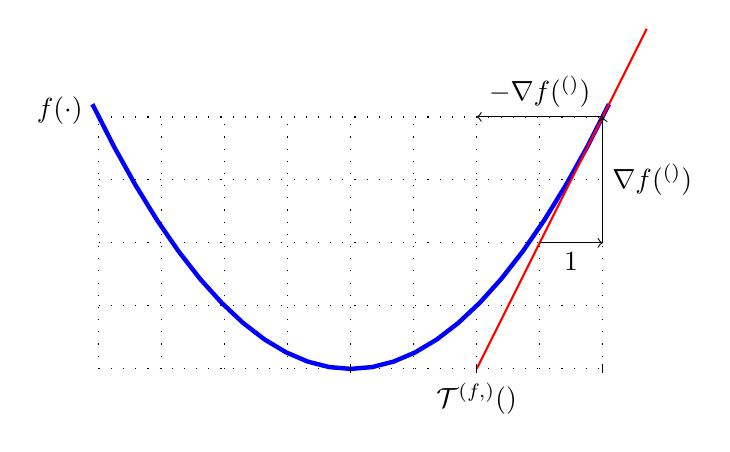
\begin{tikzpicture}[scale=0.8]
					\draw[loosely dotted] (-4,0) grid (4,4);
					\draw[blue, ultra thick, domain=-4.1:4.1] plot (\x,  {(1/4)*\x*\x});
					\draw[red, thick, domain=2:4.7] plot (\x,  {2*\x - 4});
					\draw[<-] (4,4) -- node[right] {$\nabla f(\weights^{(\itercntr)})$} (4,2);
					\draw[->] (4,4) -- node[above] {$-\lrate \nabla f(\weights^{(\itercntr)})$} (2,4);
					\draw[<-] (4,2) -- node[below] {$1$} (3,2) ;
					%\draw[->] (-4.25,0) -- (4.25,0) node[right] {$a$};
					\node[left] at (-4.1, 4.1) {$f(\cdot)$}; 
					\draw[shift={(0,0)}] (0pt,2pt) -- (0pt,-2pt) node[below] {$\overline{\weights}$};
					\draw[shift={(4,0)}] (0pt,2pt) -- (0pt,-2pt) node[below] {$\weights$};
					\draw[shift={(2,0)}] (0pt,2pt) -- (0pt,-2pt) node[below] {$\mathcal{T}^{(f,\lrate)}(\weights)$};
				\end{tikzpicture}
			\end{center}
			\caption{The basic \gls{gradient} step \eqref{equ_def_gd_basic_dict} maps a given vector $\weights$ 
			to the updated vector $\weights'$. It defines an operator 
			$\mathcal{T}^{(f,\lrate)}(\cdot): \mathbb{R}^{\nrfeatures} \rightarrow \mathbb{R}^{\nrfeatures}:
			 \weights \mapsto \widehat{\weights}$.}
			\label{fig_basic_GD_step_single_dict}
		\end{figure}
		Note that the \gls{gradient} step \eqref{equ_def_gd_basic_dict} optimizes locally - 
		in a \gls{neighborhood} whose size is determined by the \gls{stepsize} $\lrate$ - a linear approximation 
		to the \gls{function} $f(\cdot)$. A natural \gls{generalization} of \eqref{equ_def_gd_basic_dict} is to locally 
		optimize the \gls{function} itself - instead of its linear approximation - such that
		\begin{align} 
		\label{equ_approx_gd_step_dict}
		\widehat{\weights} = \argmin_{\weights' \in \mathbb{R}^{\dimlocalmodel}} f(\weights')\!+\!(1/\lrate)\normgeneric{\weights-\weights'}{2}^2. 
		\end{align}
		We intentionally use the same symbol $\lrate$ for the \gls{parameter} in \eqref{equ_approx_gd_step_dict} 
		as we used for the \gls{stepsize} in \eqref{equ_def_gd_basic_dict}. The larger the $\lrate$ we choose in 
		\eqref{equ_approx_gd_step_dict}, the more progress the update will make towards reducing the 
		\gls{function} value $f(\widehat{\weights})$. Note that, much like the \gls{gradient} step \eqref{equ_def_gd_basic_dict}, 
		also the update \eqref{equ_approx_gd_step_dict} defines an operator 
		that is parametrized by the \gls{function} $f(\cdot)$ and the \gls{learnrate} $\lrate$. For a \gls{convex} \gls{function}  
		$f(\cdot)$, this operator is known as the \gls{proxop} of $f(\cdot)$ \cite{ProximalMethods}. 
					\\ 
		See also: \gls{differentiable}, \gls{function}, \gls{gradient}, \gls{stepsize}, \gls{neighborhood}, \gls{generalization}, \gls{parameter}, \gls{learnrate}, \gls{convex}, \gls{proxop}.},
	first={gradient step},
	firstplural={gradient steps},
	plural={gradient steps},
	text={gradient step}
}

\newglossaryentry{contractop}
{name={contraction operator},
	description={An\index{contraction operator} operator $\fixedpointop: \mathbb{R}^{\nrfeatures} \rightarrow \mathbb{R}^{\nrfeatures}$
		is a contraction if, for some $\contractfac \in [0,1)$,
		\begin{equation} 
			\nonumber
			\normgeneric{ \fixedpointop \weights\!-\!\fixedpointop \weights'}{2}  \leq  \contractfac	\normgeneric{\weights\!-\!\weights'}{2} \mbox{ holds for any } \weights,\weights' \in \mathbb{R}^{\nrfeatures}.
		\end{equation}
	},
	first={contraction operator},
	text={contraction operator}, 
	firstplural={contraction operators}, 
	plural={contraction operators}
}
	

\newglossaryentry{proxop}
{name={proximal operator},
	description={Given\index{proximal operator} a \gls{convex} 
		\gls{function} $f(\weights')$, we define its proximal operator as \cite{ProximalMethods}, \cite{Bauschke:2017} 
		$$\proximityop{f(\cdot)}{\weights}{\rho}\defeq \argmin_{\weights' \in \mathbb{R}^{\dimlocalmodel}} \bigg[ f(\weights')\!+\!(\rho/2) \normgeneric{\weights- \weights'}{2}^{2}\bigg] \mbox{ with } \rho > 0. $$ 
		As illustrated in Figure \ref{fig_proxoperator_opt_dict}, evaluating the proximal operator 
		amounts to minimizing a penalized variant of $f(\weights')$. The penalty term is the 
		scaled squared Euclidean distance to a given vector $\weights$ (which is the input to the proximal operator). 
		The proximal operator can be interpreted as a \gls{generalization} of the \gls{gradstep}, which is defined 
		for a \gls{smooth} \gls{convex} \gls{function} $f(\weights')$. Indeed, taking a 
		\gls{gradstep} with \gls{stepsize} $\lrate$ at the current vector $\weights$ 
		is the same as applying the proximal operator of the \gls{function} $\tilde{f}(\weights')= \big( \nabla f(\weights)\big)^{T} (\weights'-\weights)$ 
		and using $\rho=1/\lrate$.
			\begin{figure}[H]
			\begin{center}
				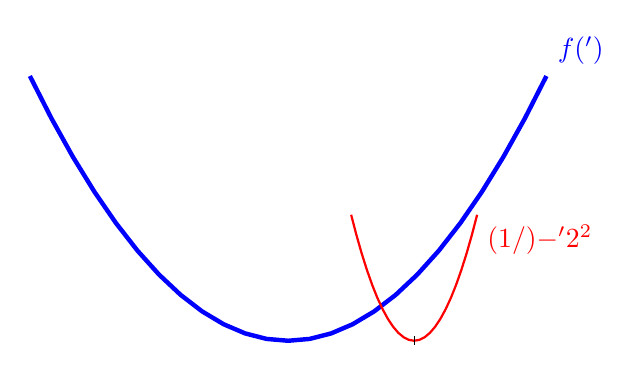
\begin{tikzpicture}[scale=0.8]
					% Original quadratic function
					\draw[blue, ultra thick, domain=-4.1:4.1] plot (\x, {(1/4)*\x*\x}) node[above right] {$f(\weights')$};		
					% Quadratic function with larger curvature, centered at w = 2
					\draw[red, thick, domain=1:3] plot (\x, {2*(\x - 2)*(\x - 2)}) node[below right] {$(1/\lrate)\normgeneric{\weights-\weights'}{2}^{2}$};
					% Axes
					% Minimum point of second curve
					\draw[shift={(2,0)}] (0pt,2pt) -- (0pt,-2pt) node[below] {$\weights$};
					%\node at (2,0.5) [anchor=north] {$\weights$};
				\end{tikzpicture}
			\end{center}
			\caption{The proximal operator updates a vector $\weights$ by minimizing a penalized version 
				of the \gls{function} $f(\cdot)$. The penalty term is the scaled squared Euclidean distance 
				between the optimization variable $\weights'$ and the given vector $\weights$.	\label{fig_proxoperator_opt_dict}}
		\end{figure}
		See also: \gls{convex}, \gls{function}, \gls{generalization}, \gls{gradstep}, \gls{smooth}, \gls{stepsize}.},
	first={proximal operator},
	text={proximal operator}
}

\newglossaryentry{proximable}
{name={proximable},
	description={A\index{proximable} 
		\gls{convex} \gls{function} for which the \gls{proxop} can be computed efficiently is 
		sometimes referred to as proximable or simple \cite{Condat2013}.
					\\ 
		See also: \gls{convex}, \gls{function}, \gls{proxop}.},
	first={proximable},
	text={proximable}
}


\newglossaryentry{connected}
{name={connected graph}, 
	description={An\index{connected graph} 
		undirected \gls{graph} $\graph=\pair{\nodes}{\edges}$ is connected\index{connected graph} if every 
		non-empty subset $\nodes' \subset \nodes$ has at least one edge connecting it to $\nodes \setminus \nodes'$.
					\\ 
		See also: \gls{graph}.}, 
	first={connected graph},
	text={connected graph}
}
	
	
\newglossaryentry{mvndist}
{name={multivariate normal distribution}, 
	description={The\index{multivariate normal distribution} multivariate normal distribution, 
 		which is denoted $\mvnormal{\meanvecgeneric}{\covmtxgeneric}$, is a fundamental \gls{probmodel} 
 		for numerical \glspl{featurevec} of fixed dimension $\nrfeatures$. 
 		It defines a family of \glspl{probdist} over vector-valued \glspl{rv} 
 		$\featurevec \in \mathbb{R}^{\nrfeatures}$~\cite{BertsekasProb}, \cite{GrayProbBook}, \cite{Lapidoth09}. 
 		Each distribution in this family is fully specified by its \gls{mean} vector 
 		$\meanvecgeneric \in \mathbb{R}^{\nrfeatures}$ and \gls{covmtx} $\covmtxgeneric \in \mathbb{R}^{\nrfeatures \times \nrfeatures}$. 
 		When the \gls{covmtx} $\covmtxgeneric$ is invertible, its \gls{probdist} is 
 		fully characterized by the following \gls{pdf}:
 		\[
 		p(\featurevec) = 
 		\frac{1}{\sqrt{(2\pi)^{\nrfeatures} \determinant{\covmtxgeneric}}} 
 		\exp\left( -\frac{1}{2} 
 		(\featurevec - \meanvecgeneric)^T \covmtxgeneric^{-1} 
 		(\featurevec - \meanvecgeneric) \right).
 		\]
 		Note that the \gls{pdf} is only defined when $\covmtxgeneric$ is invertible.
     		More generally, any \gls{rv} $\featurevec \sim \mvnormal{\meanvecgeneric}{\covmtxgeneric}$ 
     		admits the following innovation representation:
		\[\featurevec \!=\! \mA \vz \!+\!\meanvecgeneric,
		\]
		where $\vz \sim \mvnormal{\mathbf{0}}{\mathbf{I}}$ is a \gls{stdnormvec} 
		and $\mA \in \mathbb{R}^{\nrfeatures \times \nrfeatures}$ satisfies $\mA \mA^T = \covmtxgeneric$. 
		This innovation representation is valid even when the \gls{covmtx} $\covmtxgeneric$ is singular, 
		in which case $\mA$ is not necessarily full-rank \cite[Ch. 23]{Lapidoth2017}.\\ 
		The family of multivariate normal distributions is exceptional among \glspl{probmodel} for numerical 
		quantities at least for the following reasons. First, the family is closed under affine transformations, i.e., 
		\[ 
		\featurevec \sim \mathcal{N}(\meanvecgeneric,\covmtxgeneric) \mbox{ implies } 
		\mB\featurevec\!+\!\vc \sim \mathcal{N}\big( \mB\meanvecgeneric+\vc,\mB \covmtxgeneric \mB^{T} \big). 
		\]
		Second, the \gls{probdist} $\mathcal{N}(\mathbf{0},\covmtxgeneric)$ maximizes the differential \gls{entropy} 
		among all distributions with the same \gls{covmtx} $\covmtxgeneric$ \cite{coverthomas}. 
		\\ 
		See also: \gls{probmodel}, \gls{featurevec}, \gls{probdist}, \gls{rv}, \gls{covmtx}, \gls{pdf}, \gls{stdnormvec}, \gls{gaussrv}, \gls{mean}, \gls{entropy}.}, 
	first={multivariate normal distribution},
	text={multivariate normal distribution}
}

\newglossaryentry{stdnormvec}
{name={standard normal vector}, 
	description={A\index{standard normal vector} standard normal vector is a random vector $\vx=\big(x_{1},\ldots,x_{\nrfeatures}\big)^{T}$ 
		whose entries are \gls{iid} \glspl{gaussrv} $x_{\featureidx} \sim \mathcal{N}(0,1)$. 
		It is a special case of a \gls{mvndist}, $\vx \sim \mathcal(\mathbf{0},\mathbf{I})$.
		\\ 
		See also: \gls{iid}, \gls{gaussrv}, \gls{mvndist}, \gls{rv}.}, 
	first={standard normal vector},
	text={standard normal vector}
}

\newglossaryentry{statasp}
{name={statistical aspects}, 
	description={By statistical aspects\index{statistical aspects} 
		of an \gls{ml} method, we refer to (properties of) the \gls{probdist} of its output 
		under a \gls{probmodel} for the \gls{data} fed into the method.
					\\ 
		See also: \gls{ml}, \gls{probdist}, \gls{probmodel}, \gls{data}.},
	first={statistical aspects},
	text={statistical aspects}
}

\newglossaryentry{compasp}
{name={computational aspects}, 
	description={By computational 
		aspects\index{computational aspects} of an \gls{ml} method, we mainly refer to the computational 
		resources required for its implementation. For example, if an \gls{ml} method uses iterative 
		optimization techniques to solve \gls{erm}, then its computational aspects include: 1) how 
		many arithmetic operations are needed to implement a single iteration (i.e., a \gls{gradstep}); 
		and 2) how many iterations are needed to obtain useful \gls{modelparams}. One important 
		example of an iterative optimization technique is \gls{gd}.
					\\ 
		See also: \gls{ml}, \gls{erm}, \gls{gradstep}, \gls{modelparams}, \gls{gd}.}, 
	first={computational aspects},
	text={computational aspects}
}

\newglossaryentry{zerooneloss}{name={$\bf 0/1$ loss},
	description={The $0/1$ \gls{loss}\index{$0/1$ loss} $\lossfunczo{\pair{\featurevec}{\truelabel}}{\hypothesis}$ 
		measures the quality of a \gls{classifier} $\hypothesis(\featurevec)$ that delivers a 
		\gls{prediction} $\predictedlabel$ (e.g., via thresholding \eqref{equ_def_threshold_bin_classifier_dict}) 
		for the \gls{label} $\truelabel$ of a \gls{datapoint} with \glspl{feature} $\featurevec$. It is equal to $0$ if 
		the \gls{prediction} is correct, i.e., 
		$\lossfunczo{\pair{\featurevec}{\truelabel}}{\hypothesis}=0$ when $\predictedlabel=\truelabel$. It is 
		equal to $1$ if the \gls{prediction} is wrong, i.e., $\lossfunczo{\pair{\featurevec}{\truelabel}}{\hypothesis}=1$ 
		when $\predictedlabel\neq\truelabel$.
				\\ 
		See also: \gls{loss}, \gls{classifier}, \gls{prediction}, \gls{label}, \gls{datapoint}, \gls{feature}.},
	sort=zerooneloss, 
    	first={$0/1$ loss},
	text={$0/1$ loss}
}

\newglossaryentry{probability}
{name={probability}, 
	description={We\index{probability} assign a probability value, typically chosen in the 
		interval $[0,1]$, to each event that might occur in a random experiment 
		\cite{BillingsleyProbMeasure}, \cite{BertsekasProb}, \cite{HalmosMeasure},  \cite{KallenbergBook}.},
	first={probability},
	firstplural={probabilities},
	plural={probabilities},
	text={probability}
}
	
\newglossaryentry{underfitting}
{name={underfitting},
	description={Consider\index{underfitting} 
		an \gls{ml} method that uses \gls{erm} to learn a \gls{hypothesis} with the \gls{minimum} \gls{emprisk} 
		on a given \gls{trainset}. Such a method is underfitting the \gls{trainset} if it is 
		not able to learn a \gls{hypothesis} with a sufficiently small \gls{emprisk} on the \gls{trainset}. 
		If a method is underfitting, it will typically also not be able to learn a \gls{hypothesis} with 
		a small \gls{risk}.
					\\ 
		See also: \gls{ml}, \gls{erm}, \gls{hypothesis}, \gls{minimum}, \gls{emprisk}, \gls{trainset}, \gls{risk}.},
	first={underfitting},
	text={underfitting}
}

\newglossaryentry{overfitting}
{name={overfitting},
	description={Consider\index{overfitting} an 
		\gls{ml} method that uses \gls{erm} to learn a \gls{hypothesis} with the \gls{minimum} \gls{emprisk} on 
		a given \gls{trainset}. Such a method is overfitting the \gls{trainset} if it learns 
		a \gls{hypothesis} with a small \gls{emprisk} on the \gls{trainset} but a significantly larger \gls{loss} outside the \gls{trainset}.
					\\ 
		See also: \gls{generalization}, \gls{erm},  \gls{validation}, \gls{gengap}.},
	first={overfitting},
	text={overfitting}
}

\newglossaryentry{gdpr}
{name={general data protection regulation (GDPR)},
	description={The\index{general data protection regulation (GDPR)} GDPR
			was enacted by the European Union (EU), effective from May 25, 2018 \cite{GDPR2016}. 
			It safeguards the privacy and \gls{data} rights of individuals in the EU. 
			The GDPR has significant implications for how \gls{data} is collected, stored, and used in \gls{ml}  
			applications. Key provisions include the following:
			\begin{itemize}
				\item \Gls{dataminprinc}: \gls{ml} systems should only use the necessary amount of personal 
				\gls{data} for their purpose.
				\item \Gls{transparency} and \gls{explainability}: \gls{ml} systems should enable their users to 
				understand how the systems make decisions that impact the users.
				\item \Gls{data} subject rights: Users should get an opportunity to access, rectify, and delete their personal \gls{data}, as well as to object to automated decision-making and profiling.
				\item Accountability: Organizations must ensure robust \gls{data} security and demonstrate 
				compliance through documentation and regular audits.
			\end{itemize}
		See also: \gls{data}, \gls{ml}, \gls{dataminprinc}, \gls{transparency}, \gls{explainability}.}, 
	first={general data protection regulation (GDPR)},
	text={GDPR}
}
	
\newglossaryentry{gaussrv}
{name={Gaussian random variable (Gaussian RV)}, 
	plural={Gaussian RVs}, 
	description={A \index{Gaussian random variable (Gaussian RV)} standard Gaussian \gls{rv} is a 
		real-valued \gls{rv} $x$ with \gls{pdf} \cite{BertsekasProb}, \cite{GrayProbBook}, \cite{papoulis}
		\begin{equation}
			\nonumber
			p(x) = \frac{1}{\sqrt{2\pi}} \exp^{-x^2/2}. 
		\end{equation}
		Given a standard Gaussian \gls{rv} $x$, we can construct a general Gaussian \gls{rv} $x'$ with 
		\gls{mean} $\mu$ and \gls{variance} $\sigma^2$ via $x' \defeq \sigma x + \mu$. The \gls{probdist} of a 
		Gaussian \gls{rv} is referred to as normal distribution, denoted $\mathcal{N}(\mu, \sigma^2)$. 
		\\ 
		A Gaussian random vector $\featurevec \in \mathbb{R}^{\featuredim}$ with 
		\gls{covmtx} $\mathbf{C}$ and \gls{mean} ${\bm \mu}$ can be constructed as \cite{GrayProbBook}, \cite{papoulis}, \cite{Lapidoth09}
		\[
		\featurevec \defeq \mathbf{A} \vz + {\bm \mu},
		\]
		where $\vz \defeq \big( z_{1}, \ldots, z_{\featuredim} \big)^{T}$ is a vector of \gls{iid} standard Gaussian \glspl{rv}, 
		and $\mA \in \mathbb{R}^{\featuredim \times \featuredim}$ is any matrix satisfying $\mA \mA^{T} = \mC$. 
		The \gls{probdist} of a 
		Gaussian random vector is referred to as the \gls{mvndist}, denoted $\mathcal{N}({\bm \mu}, \mathbf{C})$.
		\\
		Gaussian random vectors arise as finite-dimensional marginals of \glspl{GaussProc}, which define 
		consistent joint Gaussian distributions over arbitrary (potentially infinite) index sets \cite{Rasmussen2006Gaussian}. 
  		\\
        		Gaussian \glspl{rv} are widely used \glspl{probmodel} in the statistical analysis of 
        		\gls{ml} methods. Their significance arises partly from the \gls{clt}, which is a mathematically 
        		precise formulation of the following rule-of-thumb: the average of a large number of 
        		independent \glspl{rv} (not necessarily Gaussian themselves) tends towards a Gaussian \gls{rv} \cite{ross2013first}.
		\\ 
		Compared to other \glspl{probdist}, the \gls{mvndist} is also distinct in that—in a mathematically 
		precise sense—represents maximum \gls{uncertainty}. Among all vector-valued \glspl{rv} with 
		a given covariance matrix $\mC$, the \gls{rv} $\vx \sim \mathcal{N}({\bm \mu}, \mathbf{C})$ 
		maximizes differential \gls{entropy} \cite[Th. 8.6.5]{coverthomas}. This makes \glspl{GaussProc} 
		a natural choice for capturing \gls{uncertainty} (or lack of knowledge) in the absence of additional 
		structural information.
		\\ 
		See also: \gls{mvndist}, \gls{GaussProc}, \gls{probmodel}, \gls{clt}, \gls{entropy}.
	},
	first={Gaussian random variable (Gaussian RV)},
	text={Gaussian RV}
}
	
\newglossaryentry{clt}
{name={central limit theorem (CLT)},
	description={ Consider a sequence of \gls{iid} \glspl{rv} \( \feature^{(\sampleidx)} \), for \( \sampleidx = 1, 2, \ldots \), 
		each with \gls{mean} zero and finite \gls{variance} \( \sigma^2 > 0 \). 
		The \index{central limit theorem (CLT)} CLT states that the normalized sum 
		\[
		s^{(\samplesize)} \defeq \frac{1}{\sqrt{\samplesize}} \sum_{\sampleidx = 1}^{\samplesize} \feature^{(\sampleidx)} 
		\]
		converges in distribution to a \gls{gaussrv} with \gls{mean} zero and \gls{variance} \( \sigma^2 \) as \( \samplesize \to \infty \) \cite[Proposition~2.17]{AsympVanderVaartBook}.
		One elegant way to derive the CLT is via the \gls{characteristicfunc} of the normalized sum \( s^{(\samplesize)} \). 
		Let $ \phi(t) = \expect \big\{ \exp \big( j t \feature \big) \big\}$ (with the imaginary unit $j = \sqrt{-1}$) 
		be the common \gls{characteristicfunc} of each summand $\feature^{(\sampleidx)}$, and let \( \phi^{(\samplesize)}(t) \) 
		denote the \gls{characteristicfunc} of \( s^{(\samplesize)} \). Define an operator \( \mathcal{T} \) acting on \glspl{characteristicfunc} 
		such that
		\[
		\phi^{(\samplesize)}(t) = \mathcal{T}(\phi^{(\samplesize-1)})(t) \defeq \phi\left( \frac{t}{\sqrt{\samplesize}} \right) \cdot \phi^{(\samplesize-1)}\left( \frac{\sqrt{\samplesize-1}}{\sqrt{\samplesize}} t \right).
		\]
		This \gls{fixedpointiter} captures the effect of recursively adding an \gls{iid} \gls{rv} $\featurevec^{(\samplesize)}$ 
		and rescaling. Iteratively applying \( \mathcal{T} \) leads to convergence of \( \phi^{(\samplesize)}(t) \) toward the fixed point
		\[
		\phi^*(t) = e^{-t^2 \sigma^2 / 2},
		\]
		which is the \gls{characteristicfunc} of a \gls{gaussrv} with \gls{mean} zero and \gls{variance} 
		\( \sigma^2 \). Generalizations of the CLT allow for dependent or non-identically distributed \glspl{rv} \cite[Section~2.8]{AsympVanderVaartBook}.
\begin{figure}
	\centering
	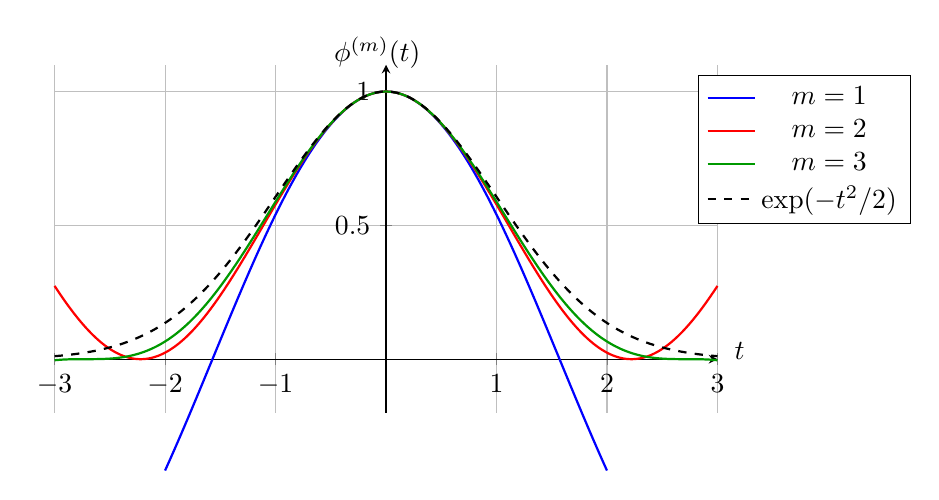
\begin{tikzpicture}
		\begin{axis}[
			width=10cm,
			height=6cm,
			xlabel={},
			ylabel={},
			legend style={at={(0.97,0.97)}, anchor=north west},
			domain=-3:3,
			ylabel style={
				yshift=10pt   % shift label up by 10pt
			},
			samples=400,
			ymin=-0.2, ymax=1.1,
			axis lines=middle,
			  clip=false,
			grid=both,
			]
		\addplot[thick, blue,domain=-2:2] {cos(x/sqrt(1) r)^1};
		\addlegendentry{$m=1$}
		\addplot[thick, red] {cos(x/sqrt(2) r)^2};
		\addlegendentry{$m=2$}
		\addplot[thick, green!60!black] {cos(x/sqrt(3) r)^3};
		\addlegendentry{$m=3$}
		\addplot[thick, dashed, black] {exp(-x^2/2)};
		\addlegendentry{$\exp(-t^2/2)$}
		\node[anchor=south, rotate=0] at (axis cs:-0.08,1.05) {$\phi^{(m)}(t)$};
		\node[anchor=north, rotate=0] at (axis cs: 3.2,0.1) {$t$};
		\end{axis}
	\end{tikzpicture}
	\caption{\Glspl{characteristicfunc} of normalized sums of \gls{iid} \glspl{rv} $x^{(\sampleidx)} \in \{-1,1\}$ 
		for $\sampleidx=1,\ldots,\samplesize$ compared to the Gaussian limit.}
\end{figure}
		\\ 
		See also: \gls{rv}, \gls{gaussrv}.},
	first={central limit theorem (CLT)},
	text={CLT}
}


\newglossaryentry{GaussProc}
{name={Gaussian process (GP)},
  description={A \index{Gaussian Process (GP)}GP is a collection of \glspl{rv} 
  	$\{f(\featurevec)\}_{\featurevec \in \featurespace}$ indexed by input values $\featurevec$ 
  	from some input space $\featurespace$, such that, for any finite subset 
  	$\featurevec^{(1)}, \ldots, \featurevec^{(\samplesize)} \in \featurespace$, 
  	the corresponding \glspl{rv} $f(\featurevec^{(1)}, \ldots, \featurevec^{(\samplesize)}$ have a joint 
  	multivariate Gaussian distribution:
  	\[
  	\left( f(\featurevec^{(1)}, \ldots, \featurevec^{(\samplesize)} \right) \sim \mathcal{N}(\boldsymbol{\mu}, \mathbf{K}).
  	\]
  	For a fixed input space $\featurespace$, a GP is fully specified (or parametrized) by 
  	\begin{itemize}
  		\item a \gls{mean} \gls{function} $\mu(\featurevec) = \expect\{ f(\featurevec)\}$
  		\item and a covariance \gls{function} $\kernelmap{\featurevec}{\featurevec'}= \expect\{ \big(f(\featurevec)-\mu(\featurevec)\big) \big(f(\featurevec')-\mu(\featurevec')\big) \big\}$.
  	\end{itemize}
  	\text{Example:} We can interpret the temperature distribution across Finland (at a specific 
  	point in time) as the \gls{realization} of a GP $f(\featurevec)$, where each input $\featurevec = (\text{lat}, \text{lon})$ 
  	denotes a geographic location. Temperature observations from \gls{fmi} weather stations provide 
  	\glspl{sample} of $f(\featurevec)$ at specific locations (see Figure \ref{fig_gp_FMI_dict}). A GP allows us to 
  	predict the temperature nearby \gls{fmi} weather stations and to quantify the \gls{uncertainty} 
  	of these predictions. 
  	\begin{figure}[H]
  	\begin{center}
  \begin{tikzpicture}
\begin{axis}[
	axis equal,
	hide axis,
	scale=1.2,
	xmin=17, xmax=32,
	ymin=55, ymax=71,
%	width=15cm,
%	height=20cm,
	clip=true
	]
	% --- Finland border (polyline) ---
	\addplot[
	color=black,
	thick
	] table [x=lon, y=lat, col sep=comma] {assets/finland_border.csv};
	% --- FMI sample stations ---
	\addplot[
	only marks,
	mark=*,
	mark options={fill=blue},
	color=black
	] table [x=lon, y=lat, col sep=comma] {assets/fmi_stations_subset.csv};
	% Draw manual axes
	\draw[->, thick] (axis cs:19,59) -- (axis cs:25.5,59) node[anchor=west] {lon};
	\draw[->, thick] (axis cs:19,59) -- (axis cs:19,65.5) node[anchor=south] {lat};
\end{axis}
\end{tikzpicture}
\vspace*{-15mm}
\end{center}
\caption{We can interpret the temperature distribution over Finland as a \gls{realization} 
	of a GP indexed by geographic coordinates and sampled at \gls{fmi} weather stations (indicated by 
	blue dots). \label{fig_gp_FMI_dict}}
\end{figure}
See also: \gls{rv}, \gls{mean}, \gls{function}, \gls{realization}, \gls{fmi}, \gls{sample}, \gls{uncertainty}.}, 
first={GP}, 
text={GP}
}

\newglossaryentry{trustAI}
{name={trustworthy artificial intelligence (trustworthy AI)},
	description={Besides the \gls{compasp} and \gls{statasp}, a third main design aspect of 
		\gls{ml} methods is their trustworthiness\index{trustworthy artificial intelligence (trustworthy AI)} \cite{pfau2024engineeringtrustworthyaideveloper}. 
		The EU has put forward seven key requirements (KRs) for trustworthy 
		\gls{ai} (that typically build on \gls{ml} methods) \cite{ALTAIEU}: 
	\begin{enumerate}[label=\arabic*)]
		\item KR1 - Human agency and oversight;
		\item KR2 - Technical \gls{robustness} and safety;
		\item KR3 - Privacy and \gls{data} governance;
		\item KR4 - \Gls{transparency};
		\item KR5 - Diversity, non-discrimination and fairness; 
		\item KR6 - Societal and environmental well-being;
		\item KR7 - Accountability. 
	\end{enumerate}
		See also: \gls{compasp}, \gls{statasp}, \gls{ml}, \gls{ai}, \gls{robustness}, \gls{data}, \gls{transparency}.},
	first={trustworthy artificial intelligence (trustworthy AI)},
	text={trustworthy AI}
}

\newglossaryentry{sqerrloss}
{name={squared error loss},
	description={The squared 
		error\index{squared error loss} \gls{loss} measures the \gls{prediction} error of a 
		\gls{hypothesis} $\hypothesis$ when predicting a numeric \gls{label} $\truelabel \in \mathbb{R}$ 
		from the \glspl{feature} $\featurevec$ of a \gls{datapoint}. It is defined as 
\begin{equation} 
	\nonumber
	\lossfunc{(\featurevec,\truelabel)}{\hypothesis} \defeq \big(\truelabel - \underbrace{\hypothesis(\featurevec)}_{=\predictedlabel} \big)^{2}. 
\end{equation} 
			\\ 
		See also: \gls{loss}, \gls{prediction}, \gls{hypothesis}, \gls{label}, \gls{feature}, \gls{datapoint}.},
	first={squared error loss},
	text={squared error loss}
}


 \newglossaryentry{projection}
 {name={projection}, 
       description={Consider\index{projection} a subset $\paramspace \subseteq \mathbb{R}^{\dimlocalmodel}$ of 
	   the $\dimlocalmodel$-dimensional \gls{euclidspace}. We define the projection $\projection{\paramspace}{\weights}$
	   of a vector $\weights \in \mathbb{R}^{\dimlocalmodel}$ onto $\paramspace$ as
	   \begin{equation} 
   	   	\label{equ_def_proj_generic_dict}
  	    	\projection{\paramspace}{\weights} = \argmin_{\weights' \in \paramspace} \normgeneric{\weights - \weights'}{2}. 
        	    \end{equation}
	    In other words, $\projection{\paramspace}{\weights}$ is the vector in $\paramspace$ 
	    which is closest to $\weights$. The projection is only well-defined for subsets $\paramspace$ 
	    for which the above \gls{minimum} exists \cite{BoydConvexBook}.
		 			\\ 
	    See also: \gls{euclidspace}, \gls{minimum}.},
	first={projection},
	text={projection}
}


\newglossaryentry{projgd}
{name={projected gradient descent (projected GD)},
description={Consider an \gls{erm}-based method that uses a parametrized \gls{model} with  
\gls{paramspace} $\paramspace \subseteq \mathbb{R}^{\dimlocalmodel}$. Even if 
the \gls{objfunc} of \gls{erm} is \gls{smooth}, we cannot use basic \gls{gd}, as 
it does not take into account contraints on the optimization variable (i.e., the \gls{modelparams}). 
Projected\index{projected gradient descent (projected GD)} \gls{gd} 
extends basic \gls{gd} to handle constraints on the optimization variable (i.e., the \gls{modelparams}). 
A single iteration of projected \gls{gd} consists of first taking a \gls{gradstep} 
and then projecting the result back onto the \gls{paramspace}.
\begin{figure}[H]
	\begin{center}
		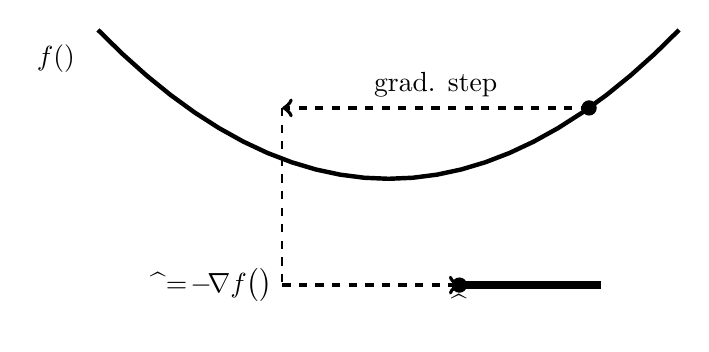
\begin{tikzpicture}[scale=0.9]
			\node [right] at (-5.1,1.7) {$f(\weights)$} ;
			\draw[ultra thick, domain=-4.1:4.1] plot (\x,  {(1/8)*\x*\x});
		%	\draw[dashed, thick, domain=1:3.6] plot (\x,  {\x - 1}) node[right] {$ f\big(\weights^{(\itercntr)}\big)\!+\!\big(\weights\!-\!\weights^{(\itercntr)}\big)^{T} \nabla f\big(\weights^{(\itercntr)}\big)$};
			\draw [fill] (2.83,1) circle [radius=0.1] node[right] {$\weights$};
			\draw[line width =0.5mm,dashed,->] (2.83,1) -- node[midway,above] {grad. step} (-1.5,1);
			\draw[line width =0.2mm,dashed] (-1.5,1) --(-1.5,-1.5)  node [below, left]{$\widehat{\weights}=\weights\!-\!\lrate \nabla f\big(\weights\big)$} ;
			\draw[line width =0.5mm,dashed,->] (-1.5,-1.5)  -- node[midway,above] {} (1,-1.5) ; 
			\draw [fill] (1,-1.5) circle [radius=0.1] node[below] {$\projection{\paramspace}{\widehat{\weights}}$};
			\draw[line width=1mm] (1,-1.5) -- (3,-1.5) node[midway, above] {$\paramspace$};
		\end{tikzpicture}
		\vspace*{-5mm}
	\end{center}
	\caption{Projected \gls{gd} augments a basic \gls{gradstep} with a \gls{projection} back 
	onto the constraint set $\paramspace$.}
	\label{fig_projected_GD_dict}
\end{figure}
		See also: \gls{erm}, \gls{model}, \gls{paramspace}, \gls{objfunc}, \gls{smooth}, \gls{gd}, \gls{modelparams}, \gls{gradstep}, \gls{projection}.},
	first={projected gradient descent (projected GD)},
	text={projected GD}
}

\newglossaryentry{diffpriv}
{name={differential privacy (DP)},
  description={Consider\index{differential privacy (DP)} some \gls{ml} method $\algomap$ 
  	that reads in a \gls{dataset} (e.g., the \gls{trainset} 
  	used for \gls{erm}) and delivers some output $\algomap(\dataset)$. The output 
  	could be either the learned \gls{modelparams} or the \glspl{prediction} for specific \glspl{datapoint}. 
  	DP is a precise measure of \gls{privleakage} incurred by revealing the 
  	output. Roughly speaking, an \gls{ml} method is differentially private if the \gls{probdist} 
  	of the output $\algomap(\dataset)$ does not change too much if the \gls{sensattr} 
  	of one \gls{datapoint} in the \gls{trainset} is changed. Note that DP 
  	builds on a \gls{probmodel} for an \gls{ml} method, i.e., we interpret its output $\algomap(\dataset)$ 
  	as the \gls{realization} of an \gls{rv}. The randomness in the output can be ensured 
  	by intentionally adding the \gls{realization} of an auxiliary \gls{rv} (i.e., adding noise) to 
  	the output of the \gls{ml} method.
				\\ 
	See also: \gls{ml}, \gls{dataset}, \gls{trainset}, \gls{erm}, \gls{modelparams}, \gls{prediction}, \gls{datapoint}, \gls{privleakage}, \gls{probdist}, \gls{sensattr}, \gls{probmodel}, \gls{realization}, \gls{rv}.}, 
  first={DP}, 
  text={DP} 
}

\newglossaryentry{robustness}
{name={robustness},
	description={Robustness\index{robustness} is a key requirement for \gls{trustAI}. It
		refers to the property of an \gls{ml} system to maintain acceptable performance even when 
		subjected to different forms of perturbations. These perturbations can be to the \glspl{feature} 
		of a \gls{datapoint} in order to manipulate the \gls{prediction} delivered by a trained \gls{ml} \gls{model}. 
		Robustness also includes the \gls{stability} of \gls{erm}-based methods against perturbations 
		of the \gls{trainset}. Such perturbations can occur within \gls{datapoisoning} \glspl{attack}. 
		\\ 
		See also: \gls{trustAI}, \gls{ml}, \gls{feature}, \gls{datapoint}, \gls{prediction}, \gls{model}, \gls{stability}, \gls{erm}, \gls{trainset}, \gls{datapoisoning}, \gls{attack}.}, 
	first={robustness}, 
	text={robustness} 
}


\newglossaryentry{stability}
{name={stability},
	description={Stability\index{stability} is a desirable property of an \gls{ml} method $\algomap$ that maps a 
		\gls{dataset} $\dataset$ (e.g., a \gls{trainset}) to an output $\algomap(\dataset)$. The output 
		$\algomap(\dataset)$ can be the learned \gls{modelparams} or the \gls{prediction} delivered 
		by the trained \gls{model} for a specific \gls{datapoint}. Intuitively, $\algomap$ is 
		stable if small changes in the input \gls{dataset} $\dataset$ lead to small changes in the 
		output $\algomap(\dataset)$. Several formal notions of stability exist that enable bounds 
		on the \gls{generalization} error or \gls{risk} of the method (see \cite[Ch.~13]{ShalevMLBook}).
		To build intuition, consider the three \glspl{dataset} depicted in Figure \ref{fig_three_data_stability_dict}, each 
		of which is equally likely under the same \gls{data}-generating \gls{probdist}. Since the 
		optimal \gls{modelparams} are determined by this underlying \gls{probdist}, an accurate 
		\gls{ml} method $\algomap$ should return the same (or very similar) output $\algomap(\dataset)$ 
		for all three \glspl{dataset}. In other words, any useful $\algomap$ must be robust to 
		variability in \gls{sample} \glspl{realization} from the same \gls{probdist}, i.e., it must be stable. 
		\begin{figure}[H]
			\centering
			\begin{tikzpicture}
				\begin{axis}[
				%title={Stem Plots of 3 Datasets},
				    axis lines=none,
					xlabel={$\sampleidx$},
					ylabel={},
					legend pos=north west,
					ymin=0, ymax=10,
					xtick={1,2,3,4,5},
				%	ymajorgrids=true,
					grid style=dashed,
					every axis plot/.append style={very thick}
					]
					% Dataset 1
					\addplot+[only marks,mark=*] coordinates {
						(1,2) (2,4) (3,3) (4,5) (5,7)
					};
				%	\addlegendentry{$\dataset^{(*)}$}
					% Dataset 2
					\addplot+[only marks,mark=square*] coordinates {
						(1,3) (2,2) (3,6) (4,4) (5,5)
					};
				%	\addlegendentry{$\dataset^{(\square)}$}
					% Dataset 3
					\addplot+[only marks,mark=triangle*] coordinates {
						(1,5) (2,7) (3,4) (4,6) (5,3)
					};
				%	\addlegendentry{$\dataset^{(\triangle)}$}
				\end{axis}
			\end{tikzpicture}
			\caption{Three \glspl{dataset} $\dataset^{(*)}$, $\dataset^{(\square)}$, and $\dataset^{(\triangle)}$, 
				each sampled independently from the same \gls{data}-generating \gls{probdist}. A stable \gls{ml} 
				method should return similar outputs when trained on any of these \glspl{dataset}. 
				\label{fig_three_data_stability_dict}}
		\end{figure}
		See also: \gls{ml}, \gls{dataset}, \gls{trainset}, \gls{modelparams}, \gls{prediction}, \gls{model}, \gls{datapoint}, \gls{generalization}, \gls{risk}, \gls{data}, \gls{probdist}, \gls{sample}, \gls{realization}.}, 
	first={stability}, 
	text={stability} 
}

\newglossaryentry{privprot}
{name={privacy protection},
     description={Consider\index{privacy protection} some \gls{ml} method $\algomap$ that reads 
	 	in a \gls{dataset} $\dataset$ and delivers some output $\algomap(\dataset)$. The output 
	 	could be the learned \gls{modelparams} $\widehat{\weights}$ or the \gls{prediction} 
	 	$\learnthypothesis(\featurevec)$ obtained for a specific \gls{datapoint} with \glspl{feature} 
	 	$\featurevec$. Many important \gls{ml} applications involve \glspl{datapoint} 
		representing humans. Each \gls{datapoint} is characterized by \glspl{feature} $\featurevec$, 
		potentially a \gls{label} $\truelabel$, and a \gls{sensattr} $\sensattr$ (e.g., a recent medical diagnosis). 
		Roughly speaking, privacy protection means that it should be impossible to infer, from the output $\algomap(\dataset)$, 
		any of the \glspl{sensattr} of \glspl{datapoint} in $\dataset$. Mathematically, privacy protection requires non-invertibility 
		of the \gls{map} $\algomap(\dataset)$. In general, just making $\algomap(\dataset)$ non-invertible 
		is typically insufficient for privacy protection. We need to make $\algomap(\dataset)$ sufficiently non-invertible. 
					\\ 
		See also: \gls{ml}, \gls{dataset}, \gls{modelparams}, \gls{prediction}, \gls{datapoint}, \gls{feature}, \gls{label}, \gls{sensattr}, \gls{map}.}, 
	first={privacy protection}, 
	text={privacy protection} 
}

\newglossaryentry{privleakage}
{name={privacy leakage},
	description={Consider\index{privacy leakage} an \gls{ml} application that processes a 
		\gls{dataset} $\dataset$ and delivers some output, such as the \glspl{prediction} 
		obtained for new \glspl{datapoint}. Privacy leakage arises 
		if the output carries information about a private (or sensitive) \gls{feature} of 
		a \gls{datapoint} (which might be a human) of $\dataset$. Based on a \gls{probmodel} 
		for the \gls{data} generation, we can measure the privacy leakage via the \gls{mutualinformation} 
		between the output and the sensitive \gls{feature}. Another quantitative measure of privacy leakage 
		is \gls{diffpriv}. The relations between different measures of privacy leakage have been 
		studied in the literature (see \cite{InfThDiffPriv}). 
				\\ 
		See also: \gls{ml}, \gls{dataset}, \gls{prediction}, \gls{datapoint}, \gls{feature}, \gls{probmodel}, \gls{data}, \gls{mutualinformation}, \gls{diffpriv}. }, 
	first={privacy leakage}, 
	text={privacy leakage} 
}


\newglossaryentry{probmodel}
{name={probabilistic model}, plural={probabilistic models},
	description={A probabilistic \gls{model}\index{probabilistic model} interprets \glspl{datapoint} 
		as \glspl{realization} of \glspl{rv} with a joint \gls{probdist}. This joint \gls{probdist} typically 
		involves \glspl{parameter} which have to be manually chosen or learned via statistical inference 
		methods such as \gls{maxlikelihood} estimation \cite{LC}.
					\\ 
		See also: \gls{model}, \gls{datapoint}, \gls{realization}, \gls{rv}, \gls{probdist}, \gls{parameter}, \gls{maxlikelihood}. }, 
	first={probabilistic model}, 
	text={probabilistic model} 
}


\newglossaryentry{mean}
{name={mean}, plural={means},
 description={The \index{mean} mean of an \gls{rv} $\featurevec$, taking 
 	values in an \gls{euclidspace} $\mathbb{R}^{\dimlocalmodel}$, is its 
 	\gls{expectation} $\expect\{\featurevec\}$. It is defined as the Lebesgue 
 	integral of $\featurevec$ with respect to the underlying \gls{probdist} $P$ (e.g., see \cite{RudinBookPrinciplesMatheAnalysis} or \cite{BillingsleyProbMeasure}), i.e.,
	\[
		\expect\{\featurevec\} = \int_{\mathbb{R}^{\dimlocalmodel}} \featurevec \, \mathrm{d}P(\featurevec).
	\] 
	Sometimes it is useful to think of the mean as the solution of the following \gls{risk} 
	minimization problem \cite{BertsekasProb}
	\[
		\expect\{\featurevec\} = \argmin_{\vc \in \mathbb{R}^{\nrfeatures}} 
		\expect \big\{\normgeneric{\featurevec - \vc}{2}^{2}\big \}.
	\] 
	We also use the term to refer to the average of a finite sequence 
	$\vx^{(1)}, \ldots, \vx^{(\samplesize)} \in \mathbb{R}^{\dimlocalmodel}$. However, 
	these two definitions are essentially the same. Indeed, we can use the sequence 
	$\vx^{(1)}, \ldots, \vx^{(\samplesize)} \in \mathbb{R}^{\dimlocalmodel}$ to construct a 
	discrete \gls{rv} $\widetilde{\vx}=\vx^{(I)}$, with the index $I$ being chosen uniformly 
	at random from the set $\{1,\ldots,\samplesize\}$. The mean of $\widetilde{\vx}$ is 
	precisely the average $\frac{1}{\samplesize} \sum_{\sampleidx=1}^{\samplesize} \vx^{(\sampleidx)}$.
			\\ 
		See also: \gls{rv}, \gls{expectation}, \gls{probdist}.}, 
		first = {mean}, text={mean} 
}

\newglossaryentry{median}
{name={median}, 
 plural={medians},
 description={A\index{median} median $\med(x)$ of a real-valued \gls{rv} $x$ 
 is any number $m \in \mathbb{R}$ such that $\prob{ x \leq m} \geq 1/2$ and $\prob{ x \geq m} \geq 1/2$ \cite{LC}. 
 \begin{figure}
	\begin{center}
	\begin{tikzpicture}
  \begin{axis}[
    axis lines=middle,
    xlabel={$m$},
    ylabel={},
    ymin=0, ymax=1.1,
    xmin=-2, xmax=6,
    xtick=\empty,
    ytick={0,1/2,1},
    domain=-2:6,
    samples=200,
    width=10cm,
    height=6cm,
    smooth,
    enlargelimits=true,
    clip=false
  ]
    % Shifted sigmoid CDF
	\addplot[thick, blue, name path=cdf] {1/(1 + exp(-(x - 1)))} node[pos=0.5, above, yshift=15pt] {$\prob{x \leq m}$};    % Vertical and horizontal ruler at F(x) = 0.5
    \draw[dashed, gray] (axis cs:1,0) -- (axis cs:1,0.5); % vertical
    \draw[dashed, gray] (axis cs:-2,0.5) -- (axis cs:1,0.5); % horizontal
    % Mark the median point
    \filldraw[red] (axis cs:1,0.5) circle (2pt);
  %  \node[below left] at (axis cs:1,0.5) {\footnotesize $(x{=}1,\ F(x){=}\tfrac{1}{2})$};
    % Label next to curve
  \end{axis}
\end{tikzpicture} 
\end{center}
 \end{figure}  
 We can define the median $\med(\dataset)$ 
 of a \gls{dataset} $\dataset = \{ x^{(1)}, \ldots, x^{(\samplesize)} \in \mathbb{R} \}$ 
 via a specific \gls{rv} $\tilde{x}$ that is naturally associated with $\dataset$. 
 In particular, this \gls{rv} is constructed by $\tilde{x} = x^{(I)}$ with the index $I$ 
 being chosen uniformly at random from the set $\{1,\ldots,\samplesize\}$, i.e., $\prob{I = \sampleidx}=1/\samplesize$ for 
 all $\sampleidx=1,\ldots,\samplesize$. If the \gls{rv} $x$ is integrable, a median of $x$ 
 is the solution of the following optimization problem: 
 $$\min_{x' \in \mathbb{R}} \expect{|x - x'|}.$$ 
 Like the \gls{mean}, also the median of a \gls{dataset} $\dataset$ can be used 
 to estimate the \glspl{parameter} of an underlying \gls{probmodel}. Compared 
 to the \gls{mean}, the median is more robust to \glspl{outlier}. For example, 
 a median of a \gls{dataset} $\dataset$ with more than one \gls{datapoint} does not 
 change even if we arbitrarily increase the largest element of $\dataset$. In contrast, 
 the \gls{mean} will increase arbitrarily.
	\begin{figure}
		\centering
		\begin{tikzpicture}[scale=0.7, y=0.5cm, x=0.5cm]
			\begin{scope}
				\foreach \x/\y in {
					1/2, 4/3, 7/4
				} {
					\draw[dashed, gray] (\x, 0) -- (\x, \y);
					\filldraw[blue] (\x, \y) circle (2pt);
					\node[circle, inner sep=0pt] (ptA\x) at (\x, \y) {};
				}
				\draw[dashed, thick, darkgreen] (0.5, 3) -- (10.5, 3) node[right] {$\med(\dataset)$};
				\node at (5.5, -4) {(a) Original \gls{dataset} $\dataset$.};
			\end{scope}
			\begin{scope}[xshift=12cm]
				\foreach \x/\y in {
					1/2, 4/3, 7/10
				} {
					\draw[dashed, gray] (\x, 0) -- (\x, \y);
					\filldraw[blue] (\x, \y) circle (2pt);
					\node[circle, inner sep=0pt] (ptB\x) at (\x, \y) {};
				}
				\draw[dashed, thick, darkgreen] (0.5, 3) -- (10.5, 3) node[right] {$\med\big(\widetilde{\dataset}\big)$};
				\node[above right=2pt and 2pt, red] at (ptB7) {outlier};
				\node at (5.5, -4) {(b) Noisy \gls{dataset} $\widetilde{\dataset}$ including an \gls{outlier}.};
			\end{scope}
		\end{tikzpicture}
		\caption{The median is robust against \gls{outlier} contamination. }
	\end{figure}
	\\ 
		See also: \gls{mean}, \gls{robustness}, \gls{outlier}.}, 
	first = {median}, 
	text={median} 
}



\newglossaryentry{variance}
{name={variance},
	description={The\index{variance} variance of a real-valued \gls{rv} $\feature$ is defined as the \gls{expectation} 
		$\expect\big\{ \big( x - \expect\{x \} \big)^{2} \big\}$ of the squared difference between $\feature$ 
		and its \gls{expectation} $\expect\{x \}$. We extend this definition to vector-valued \glspl{rv} $\featurevec$ 
		as $\expect\big\{ \big\| \featurevec - \expect\{\featurevec \} \big\|_{2}^{2} \big\}$.
					\\ 
		See also: \gls{rv}, \gls{expectation}.},
	first={variance},
	text={variance} 
}

\newglossaryentry{nn}
{name={nearest neighbor (NN)},
	description={NN\index{nearest neighbor (NN)} methods learn a \gls{hypothesis} 
		$\hypothesis: \featurespace \rightarrow \labelspace$ whose \gls{function} value $\hypothesis(\featurevec)$ 
		is solely determined by the NNs within a given \gls{dataset}. Different 
		methods use different metrics for determining the NNs. If \glspl{datapoint} 
		are characterized by numeric \glspl{featurevec}, we can use their Euclidean distances as 
		the metric.
					\\ 
		See also: \gls{hypothesis}, \gls{function}, \gls{dataset}, \gls{datapoint}, \gls{featurevec}, \gls{neighbors}.},
	first={nearest neighbor (NN)},
	text={NN} 
}

\newglossaryentry{neighborhood}
{name={neighborhood},
	description={The\index{neighborhood} neighborhood of a node $\nodeidx \in \nodes$ is 
		the subset of nodes constituted by the \gls{neighbors} of $\nodeidx$.
				\\ 
		See also: \gls{neighbors}.},
	first={neighborhood},
	text={neighborhood} 
}


\newglossaryentry{neighbors}
{name={neighbors},
	description={The\index{neighbors} neighbors of a node $\nodeidx \in \nodes$ 
		within an \gls{empgraph} are those nodes $\nodeidx' \in \nodes \setminus \{ \nodeidx\}$ that are connected (via an edge) to node $\nodeidx$.
				\\ 
		See also: \gls{empgraph}.},
	first={neighbors},
	text={neighbors} 
}

\newglossaryentry{bias}
{name={bias},
	description={Consider\index{bias} an \gls{ml} method using a parametrized \gls{hypospace} $\hypospace$. 
		It learns the \gls{modelparams} $\weights \in \mathbb{R}^{\dimlocalmodel}$ using the \gls{dataset} $$ \dataset=\big\{ \pair{\featurevec^{(\sampleidx)}}{\truelabel^{(\sampleidx)}} \big\}_{\sampleidx=1}^{\samplesize}.$$ 
		To analyze the properties of the \gls{ml} method, we typically interpret the \glspl{datapoint} as \glspl{realization} 
		of \gls{iid} \glspl{rv}, $$ \truelabel^{(\sampleidx)} = \hypothesis^{(\overline{\weights})}\big( \featurevec^{(\sampleidx)} \big) + \bm{\varepsilon}^{(\sampleidx)}, \sampleidx=1,\ldots,\samplesize.$$ 
		We can then interpret the \gls{ml} method as an estimator $\widehat{\weights}$ 
		computed from $\dataset$ (e.g., by solving \gls{erm}). The (squared) bias incurred by the estimate $\widehat{\weights}$ 
		is then defined as $\biasterm^{2} \defeq \big\| \expect \{ \widehat{\weights}  \}- \overline{\weights}\big\|_{2}^{2}$.
					\\ 
		See also: \gls{ml}, \gls{hypospace}, \gls{modelparams}, \gls{dataset}, \gls{datapoint}, \gls{realization}, \gls{iid}, \gls{rv}, \gls{erm}.},
	first={bias},
	text={bias} 
}

\newglossaryentry{classification}
{name={classification},
	description={Classification\index{classification} is the task of determining a 
 		discrete-valued \gls{label} $\truelabel$ for a given \gls{datapoint}, based solely on its 
 		\glspl{feature} $\featurevec$. The \gls{label} $\truelabel$ belongs to a finite set, such as 
 		$\truelabel \in \{-1,1\}$ or $\truelabel \in \{1,\ldots,19\}$, and represents the 
 		category to which the corresponding \gls{datapoint} belongs.
				\\ 
		See also: \gls{label}, \gls{datapoint}, \gls{feature}.},
	first={classification},
	text={classification} 
}


\newglossaryentry{privfunnel}
{name={privacy funnel},
	description={The\index{privacy funnel} privacy funnel is a method for learning privacy-friendly \glspl{feature} 
		of \glspl{datapoint} \cite{PrivacyFunnel}.
				\\ 
		See also: \gls{feature}, \gls{datapoint}.},
 	first={privacy funnel},
	text={privacy funnel} 
}


\newglossaryentry{condnr}
{name={condition number},
	description={The condition number\index{condition number} $\kappa(\mathbf{Q}) \geq 1$ of a 
		positive definite 
		matrix $\mathbf{Q} \in \mathbb{R}^{\featurelen \times \featurelen}$ is the ratio 
		$\alpha /\beta  $ between the 
		largest $\alpha$ and the smallest $\beta$ \gls{eigenvalue} of 
		$\mathbf{Q}$. The condition number is useful for the analysis of \gls{ml} methods. 
		The computational complexity of \gls{gdmethods} for \gls{linreg} crucially depends on the 
		condition number of the matrix $\mQ = \mX \mX^{T}$, with the \gls{featuremtx} $\mX$ 
		of the \gls{trainset}. Thus, from a computational perspective, we prefer \glspl{feature} of 
		\glspl{datapoint} such that $\mQ$ has a condition number close to $1$.
					\\ 
		See also: \gls{eigenvalue}, \gls{ml}, \gls{gdmethods}, \gls{linreg}, \gls{featuremtx}, \gls{trainset}, \gls{feature}, \gls{datapoint}.},
	first={condition number},
	text={condition number} 
}

\newglossaryentry{classifier}
{name={classifier},
	description={A classifier\index{classifier} is a \gls{hypothesis} (i.e., a \gls{map}) $\hypothesis(\featurevec)$ 
		used to predict a \gls{label} taking values from a finite \gls{labelspace}. We might use the 
		\gls{function} value $\hypothesis(\featurevec)$ itself as a \gls{prediction} $\predictedlabel$ for 
		the \gls{label}. However, it is customary to use a \gls{map} $\hypothesis(\cdot)$ that delivers 
		a numeric quantity. The \gls{prediction} is then obtained by a simple thresholding step. 
		For example, in a binary \gls{classification} problem with \gls{labelspace} $\labelspace \in  \{ -1,1\}$, 
		we might use a real-valued \gls{hypothesis} \gls{map} $\hypothesis(\featurevec) \in \mathbb{R}$ 
		as a classifier. A \gls{prediction} $\predictedlabel$ can then be obtained via thresholding,  
		 \begin{equation} 
		 	\label{equ_def_threshold_bin_classifier_dict}
		 	\predictedlabel =1   \mbox{ for } \hypothesis(\featurevec)\!\geq\!0 \mbox{ and } 	\predictedlabel =-1  \mbox{ otherwise.}
	 		\end{equation}
 		We can characterize a classifier by its \glspl{decisionregion} $\decreg{a}$, for 
 		every possible \gls{label} value $a \in \labelspace$.
					\\ 
		See also: \gls{hypothesis}, \gls{map}, \gls{label}, \gls{labelspace}, \gls{function}, \gls{prediction}, \gls{classification}, \gls{decisionregion}. },
	first={classifier},
	text={classifier} 
}

\newglossaryentry{emprisk}
{name={empirical risk},
  description={The empirical \gls{risk}\index{empirical risk} $\emprisk{\hypothesis}{\dataset}$ 
  	of a \gls{hypothesis} on a \gls{dataset} $\dataset$ is the average \gls{loss} incurred 
  	by $\hypothesis$ when applied to the \glspl{datapoint} in $\dataset$.
				\\ 
		See also: \gls{risk}, \gls{hypothesis}, \gls{dataset}, \gls{loss}, \gls{datapoint}.},
  first={empirical risk},
  text={empirical risk} 
}

\newglossaryentry{nodedegree}
{name={node degree},
	description={The degree\index{node degree} $\nodedegree{\nodeidx}$ of a node $\nodeidx \in \nodes$ 
		in an undirected \gls{graph} is the number of its \gls{neighbors}, i.e., $\nodedegree{\nodeidx} \defeq \big|\neighbourhood{\nodeidx}\big|$.
					\\ 
		See also: \gls{graph}, \gls{neighbors}.},
	first={node degree},
	text={node degree} 
}

\newglossaryentry{graph}
{name={graph},
	description={A graph\index{graph} $\graph = \pair{\nodes}{\edges}$ is a pair that consists of 
		a node set $\nodes$ and an edge set $\edges$. In its most general form, a graph is 
		specified by a \gls{map} that assigns each edge $\edgeidx \in \edges$ a pair of nodes \cite{RockNetworks}. 
		One important family of graphs is simple undirected graphs. A simple undirected graph 
		is obtained by identifying each edge $\edgeidx \in \edges$ with two different nodes $\{\nodeidx,\nodeidx'\}$. 
		Weighted graphs also specify numeric \gls{weights} $\edgeweight_{\edgeidx}$ for each 
		edge $\edgeidx \in \edges$.
					\\ 
		See also: \gls{map}, \gls{weights}.},
	first={graph},
	text={graph} 
}

\newglossaryentry{uncertainty}
{name={uncertainty},
	description={Uncertainty\index{uncertainty} refers to the degree of confidence—or 
		lack thereof—associated with a quantity such as a \gls{model} \gls{prediction}, \gls{parameter} estimate, or 
		observed \gls{datapoint}. In \gls{ml}, uncertainty arises from various sources, including 
		noisy \gls{data}, limited training \glspl{sample}, or ambiguity in \gls{model} assumptions. \Gls{probability} theory 
		offers a principled framework for representing and quantifying such uncertainty.
					\\ 
		See also: \gls{model}, \gls{prediction}, \gls{parameter}, \gls{datapoint}, \gls{ml}, \gls{data}, \gls{sample}, \gls{probability}.},
	first={uncertainty},
	text={uncertainty}
}

\newglossaryentry{ucb}
{name={upper confidence bound (UCB)},
	description={Consider\index{upper confidence bound (UCB)} an \gls{ml} 
		application that requires selecting, at each time step $\iteridx$, an action $\action_{\iteridx}$ 
		from a finite set of alternatives $\actionset$. The utility of selecting action $\action_{\iteridx}$ 
		is quantified by a numeric \gls{reward} signal $\reward^{(\action_{\iteridx})}$. 
		A widely used \gls{probmodel} for this type of sequential decision-making problem 
		is the \gls{stochastic} \gls{mab} setting \cite{Bubeck2012}. In this \gls{model}, 
		the \gls{reward} $\reward^{(\action)}$ is viewed as the \gls{realization} of an \gls{rv} 
		with unknown \gls{mean} $\mu^{(\action)}$. Ideally, we would always choose the 
		action with the largest expected \gls{reward} $\mu^{(\action)}$, but these 
		\glspl{mean} are unknown and must be estimated from observed \gls{data}. Simply 
		choosing the action with the largest estimate $\widehat{\mu}^{(\action)}$ can 
		lead to suboptimal outcomes due to estimation \gls{uncertainty}. The UCB strategy 
		addresses this by selecting actions not only based on their estimated \glspl{mean} but 
		also by incorporating a term that reflects the \gls{uncertainty} in these estimates—favoring 
		actions with a high potential \gls{reward} and high \gls{uncertainty}. Theoretical guarantees 
		for the performance of UCB strategies, including logarithmic \gls{regret} bounds, are established in \cite{Bubeck2012}.
					\\ 
		See also: \gls{ml}, \gls{reward}, \gls{probmodel}, \gls{stochastic}, \gls{mab}, \gls{model}, \gls{realization}, \gls{rv}, \gls{mean}, \gls{data}, \gls{uncertainty}, \gls{regret}.},
	first={upper confidence bound (UCB)},
	text={UCB} 
}

\newglossaryentry{mab}
{name={multi-armed bandit (MAB)},
	description={A MAB\index{multi-armed bandit (MAB)} problem models 
		a repeated decision-making scenario in which, at each time step $\iteridx$, a learner must 
		choose one out of several possible actions, often referred to as arms, from a finite 
		set $\actionset$. Each arm $\action \in \actionset$ yields a \gls{stochastic} \gls{reward} $\reward^{(\action)}$ 
		drawn from an unknown \gls{probdist} with \gls{mean} $\mu^{(\action)}$. 
		The learner’s goal is to maximize the cumulative \gls{reward} over time by 
		strategically balancing exploration (i.e., gathering information about 
		uncertain arms) and exploitation (i.e., selecting arms known to perform well). 
		This balance is quantified by the notion of \gls{regret}, which measures the performance 
		gap between the learner's strategy and the optimal strategy that always selects the best arm. 
		MAB problems form a foundational \gls{model} in \gls{onlinelearning}, reinforcement learning, 
		and sequential experimental design \cite{Bubeck2012}.
					\\ 
		See also: \gls{stochastic}, \gls{reward}, \gls{probdist}, \gls{mean}, \gls{regret}, \gls{model}.},
	first={MAB},
	text={MAB}
}



\newglossaryentry{optimism in the face of uncertainty}
{name={optimism in the face of uncertainty},
	description={\gls{ml}\index{optimism in the face of uncertainty} methods learn \gls{modelparams} $\weights$ 
		according to some performance criterion $\bar{f}(\weights)$. However, they usually 
		cannot access $\bar{f}(\weights)$ directly but rely on an estimate (or approximation) 
		$f(\weights)$ of $\bar{f}(\weights)$. As a case in point, \gls{erm}-based methods use 
		the average \gls{loss} on a given \gls{dataset} (i.e., the \gls{trainset}) as an estimate 
		for the \gls{risk} of a \gls{hypothesis}. Using a \gls{probmodel}, one can construct 
		a confidence interval 
		$\big[ l^{(\weights)},  u^{(\weights)} \big]$ for each choice $\weights$ for the \gls{modelparams}.
		One simple construction is $l^{(\weights)} \defeq f(\weights) - \sigma/2$, $u^{(\weights)} \defeq f(\weights)+ \sigma/2$, 
	    	with $\sigma$ being a measure of the (expected) deviation of $f(\weights)$ from $\bar{f}(\weights)$.
		We can also use other constructions for this interval as long as they ensure that $\bar{f}(\weights) \in\big[ l^{(\weights)},  u^{(\weights)} \big]$ 
		with a sufficiently high \gls{probability}. An optimist chooses the \gls{modelparams} 
		according to the most favorable—yet still plausible—value $\tilde{f}(\weights) \defeq  l^{(\weights)}$ 
		of the performance criterion. Two examples of \gls{ml} methods that use such an optimistic 
		construction of an \gls{objfunc} are \gls{srm} \cite[Ch. 11]{ShalevMLBook} and \gls{ucb} methods 
		for sequential decision making \cite[Sec. 2.2]{Bubeck2012}. 
		\begin{figure}[H]
				\begin{center}
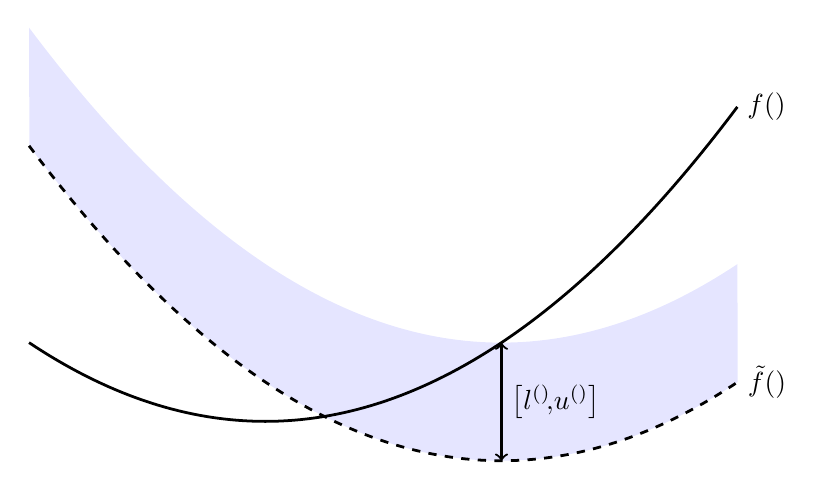
\begin{tikzpicture}[x=3cm, y=1cm]
  % Filled band around the quadratic curve with different boundary curves
\fill[blue!10] 
(-1, 5) -- plot[domain=-2:1, samples=100] ({\x+1}, {\x*\x + 1}) -- 
plot[domain=1:-2, samples=100] ({\x+1}, {\x*\x - 0.5}) -- cycle;
  \node[anchor=west] at (2, 4) {$f(\weights)$};
  \draw[line width=1, domain=-2:1, samples=100,dashed] plot  ({\x+1}, {\x*\x -0.5}) node[right] {$\tilde{f}(\weights)$};
   \draw[line width=1, domain=-1:2, samples=100] plot ({\x}, {\x*\x});
  \draw[<->, thick] (1, -0.5) -- (1, 1) node[midway, right] {$\big[ l^{(\weights)}\!,\!u^{(\weights)} \big]$};
\end{tikzpicture}
\caption{\gls{ml} methods learn \gls{modelparams} $\weights$ by using some estimate of $f(\weights)$ for 
	the ultimate performance criterion $\bar{f}(\weights)$. Using a \gls{probmodel}, one can use $f(\weights)$ to 
	construct confidence intervals $\big[ l^{(\weights)},  u^{(\weights)} \big]$ which contain $\bar{f}(\weights)$  
	with a high probability. The best plausible performance measure for a specific choice $\weights$ of \gls{modelparams} 
	is $\tilde{f}(\weights) \defeq l^{(\weights)}$.} 
	\end{center}
		\end{figure}
		See also: \gls{ml}, \gls{modelparams}, \gls{erm}, \gls{loss}, \gls{dataset}, \gls{trainset}, \gls{risk}, \gls{hypothesis}, \gls{probmodel}, \gls{probability}, \gls{objfunc}, \gls{srm}, \gls{ucb}.},
	first={optimism in the face of uncertainty},
	text={optimism in the face of uncertainty} 
}

\newglossaryentry{empgraph}
{name={federated learning network (FL network)},
	description={An \gls{fl} network\index{federated learning network (FL network)} consists of 
		an undirected weighted \gls{graph} $\graph$. The nodes of $\graph$ represent \glspl{device} 
		that can access a \gls{localdataset} and train a \gls{localmodel}. The edges of $\graph$ represent 
		communication links between \glspl{device} as well as statistical similarities between their \glspl{localdataset}. 
		A principled approach to train the \glspl{localmodel} is \gls{gtvmin}. The solutions of \gls{gtvmin} are local 
		\gls{modelparams} that optimally balance the \gls{loss} incurred on \glspl{localdataset} with their discrepancy 
		across the edges of $\graph$. 
	    			\\ 
		See also: \gls{fl}, \gls{graph}, \gls{device}, \gls{gtvmin}.},
	first={federated learning network (FL network)},
	text={FL network} 
}

\newglossaryentry{norm}
{name={norm},
	description={A norm\index{norm} is a \gls{function} that maps each (vector) element 
		of a \gls{vectorspace} to a non-negative real number. This \gls{function} must be 
		homogeneous and definite, and it must satisfy the triangle inequality \cite{HornMatAnalysis}.
		\\
		See also: \gls{function}, \gls{vectorspace}.},
	first={norm},
	text={norm} 
}

\newglossaryentry{dualnorm}
{name={dual norm},
	description={Every \gls{norm} $\normgeneric{\cdot}{}$ defined on an \gls{euclidspace} $\mathbb{R}^{\dimlocalmodel}$ 
		has an associated dual \gls{norm}, which is denoted $\normgeneric{\cdot}{*}$ and defined as 
		$\normgeneric{\vy}{*} \defeq \sup_{\norm{\vx}{} \le 1} \vy^{T} \vx$. 
		The dual \gls{norm} measures the largest possible inner product between $\vy$ 
		and any vector in the unit ball of the original \gls{norm}. For further details, see 
		\cite[Sec.~A.1.6]{BoydConvexBook}.
					\\ 
		See also: \gls{norm}, \gls{euclidspace}.},
	first={dual norm},
	text={dual norm}
}

\newglossaryentry{geometricmedian}
{name={geometric median (GM)},
	description={The GM\index{geometric median (GM)} of a set of input vectors $\vx^{(1)}, \ldots, \vx^{(\samplesize)}$ 
		in $\mathbb{R}^{\dimlocalmodel}$ is a point $\vz \in \mathbb{R}^{\dimlocalmodel}$ that 
		minimizes the sum of distances to the vectors \cite{BoydConvexBook} such that 
		\begin{equation} 
			\label{equ_geometric_median_dict}
		\vz \in \argmin_{\vy \in \mathbb{R}^{\dimlocalmodel}} \sum_{\sampleidx=1}^{\samplesize} \normgeneric{\vy - \vx^{(\sampleidx)}}{2}.
		\end{equation} 
	Figure \ref{opt_cond_GM_dict} illustrates a fundamental property of the GM:
	If $\vz$ does not coincide with any of the input vectors, then the unit vectors pointing 
	from $\vz$ to each $\vx^{(\sampleidx)}$ must sum to zero—this is the zero-\gls{subgradient}  
	(optimality) condition of \eqref{equ_geometric_median}. It turns out that the solution to 
	\eqref{equ_geometric_median_dict} cannot be arbitrarily pulled away from trustworthy input 
	vectors as long as they are the majority \cite[Th. 2.2]{Lopuhaae1991}.
	  	\begin{figure}[H]
  		\begin{center}
			\begin{tikzpicture}[scale=2, thick, >=stealth]
%				% Central model w
				\coordinate (w) at (3,0);
				\fill (w) circle (1.2pt) node[below right] {$\vz$};
% Clean nodes
				\coordinate (w2) at (0.5,0.3);
				\coordinate (w3) at (0.7,0.7);
				\fill (w2) circle (1pt) node[above left] {$\vx^{(1)}$};
				\fill (w3) circle (1pt) node[above left] {$\vx^{(2)}$};
			    \node[anchor=west] at ($(w2) +(-0.2,0.9)$) {\textbf{clean}};
%				% Dashed lines from w to good nodes
				\draw[dashed] (w) -- (w2);
				\draw[dashed] (w) -- (w3);
%				% Draw unit vectors (scaled to 1cm)
				\draw[->, thick, red] (w) -- ($(w)!1cm!(w2)$) ;
				\draw[->, thick, red] (w) -- ($(w)!1cm!(w3)$) node[pos=0.9, right,yshift=7pt] {$\frac{\vx^{(2)}- \vz}{\normgeneric{\vx^{(2)}-\vz}{2}}$};
%				\node at (-0.2,1.4) {\textbf{Clean}};
				\coordinate (w4) at (5,0.2);
				\node at (5,0.6) {\textbf{perturbed}};
				\fill (w4) circle (1pt) node[below left] {$\vx^{(3)}$};
				\draw[->, thick, red] (w) -- ($(w)!1cm!(w4)$) ;
%		% Optional dotted line from w to bad
		\end{tikzpicture}
		\caption{\label{opt_cond_GM_dict}
			Consider a solution $\vz$ of \eqref{equ_geometric_median} that does not coincide 
			with any of the input vectors. The optimality condition for \eqref{equ_geometric_median} 
			requires that the unit vectors from $\vz$ to the input vectors sum to zero.}
			\end{center}
		\end{figure}
		See also: \gls{subgradient}.},
	first={geometric median},
	text={GM}
}


\newglossaryentry{explanation}
{name={explanation},
	description={One approach to make \gls{ml} methods transparent is to provide an 
		explanation\index{explanation} along with the \gls{prediction} delivered by an 
		\gls{ml} method. Explanations can take on many different forms. An explanation 
		could be some natural text or some quantitative measure for the importance 
		of individual \glspl{feature} of a \gls{datapoint} \cite{Molnar2019}. We can also 
		use visual forms of explanations, such as intensity plots for image \gls{classification} \cite{GradCamPaper}.
					\\ 
		See also: \gls{ml}, \gls{prediction}, \gls{feature}, \gls{datapoint}, \gls{classification}.},
	first={explanation},
	text={explanation} 
}

\newglossaryentry{risk}
{name={risk},
	description={Consider\index{risk} a \gls{hypothesis} $\hypothesis$ used to predict the \gls{label} 
		$\truelabel$ of a \gls{datapoint} based on its \glspl{feature} $\featurevec$. We measure 
		the quality of a particular \gls{prediction} using a \gls{lossfunc} $\lossfunc{(\featurevec,\truelabel)}{\hypothesis}$. 
		If we interpret \glspl{datapoint} as the \glspl{realization} of \gls{iid} \glspl{rv}, 
		also the $\lossfunc{(\featurevec,\truelabel)}{\hypothesis}$ becomes the \gls{realization} 
		of an \gls{rv}. The \gls{iidasspt} allows us to define the risk of a \gls{hypothesis} 
		as the expected \gls{loss} $\expect \big\{\lossfunc{(\featurevec,\truelabel)}{\hypothesis} \big\}$. 
		Note that the risk of $\hypothesis$ depends on both the specific choice for the \gls{lossfunc} and the 
		\gls{probdist} of the \glspl{datapoint}.
					\\ 
		See also: \gls{hypothesis}, \gls{label}, \gls{datapoint}, \gls{feature}, \gls{prediction}, \gls{lossfunc}, \gls{realization}, \gls{iid} \gls{rv}, \gls{iidasspt}, \gls{loss}, \gls{probdist}.},
	first={risk},
	text={risk} 
}

\newglossaryentry{actfun}
{name={activation function},
	description={Each\index{activation function} artificial neuron within an \gls{ann} is 
		assigned an activation \gls{function} $\actfun(\cdot)$ that maps a weighted combination of 
		the neuron inputs $\feature_{1},\ldots,\feature_{\nrfeatures}$ to a single output 
		value $a = \actfun\big(\weight_{1} \feature_{1}+\ldots+\weight_{\nrfeatures} \feature_{\nrfeatures} \big)$. 
		Note that each neuron is parametrized by the \gls{weights} $\weight_{1},\ldots,\weight_{\nrfeatures}$.
					\\ 
		See also: \gls{ann}, \gls{function}, \gls{weights}.},
	first={activation function},
	text={activation function} 
}

\newglossaryentry{distributedalgorithm}
{name={distributed algorithm},
	description={A\index{distributed algorithm} distributed \gls{algorithm} is an \gls{algorithm} designed for 
		a special type of computer, i.e., a collection of interconnected computing devices (or nodes). 
		These devices communicate and coordinate their local computations by exchanging 
		messages over a network \cite{IntroDistAlg}, \cite{ParallelDistrBook}. Unlike a classical \gls{algorithm}, 
		which is implemented on a single \gls{device}, a distributed \gls{algorithm} is 
		executed concurrently on multiple \glspl{device} with computational capabilities. 
		Similar to a classical \gls{algorithm}, a distributed \gls{algorithm} can be modeled as a 
		set of potential executions. However, each execution in the distributed setting involves 
		both local computations and message-passing events. A generic execution might look as 
		follows:
		\[
		\begin{array}{l}
			\text{Node 1: } {\rm input}_1, s_1^{(1)}, s_2^{(1)}, \ldots, s_{T_1}^{(1)}, {\rm output}_1; \\
			\text{Node 2: } {\rm input}_2, s_1^{(2)}, s_2^{(2)}, \ldots, s_{T_2}^{(2)}, {\rm output}_2; \\
			\quad \vdots \\
			\text{Node N: } {\rm input}_N, s_1^{(N)}, s_2^{(N)}, \ldots, s_{T_N}^{(N)}, {\rm output}_N.
		\end{array}
		\]
		Each \gls{device} $\nodeidx$ starts from its own local input and performs a sequence of 
		intermediate computations $s_{\iteridx}^{(\nodeidx)}$ at discrete time instants $\iteridx = 1, \dots, T_\nodeidx$. 
		These computations may depend on both the previous local computations at the \gls{device} 
		and the messages received from other \glspl{device}. One important application of distributed 
		\glspl{algorithm} is in \gls{fl} where a network of \glspl{device} collaboratively trains a personal \gls{model} 
		for each \gls{device}. 
					\\ 
		See also: \gls{algorithm}, \gls{device}, \gls{fl}, \gls{model}.
		},
	first={distributed algorithm}, 
	text={distributed algorithm}
}


\newglossaryentry{algorithm}
{name={algorithm}, plural={algorithms},
 	description={An\index{algorithm} algorithm is a precise, step-by-step specification for 
  		how to produce an output from a given input within a finite number of computational steps \cite{Cormen:2022aa}. 
    		For example, an algorithm for training a \gls{linmodel} explicitly describes how to 
		transform a given \gls{trainset} into \gls{modelparams} through a sequence of \glspl{gradstep}. 
    		To study algorithms rigorously, we can represent (or approximate) them by different mathematical structures \cite{Sipser2013}. 
     		One approach is to represent an algorithm as a collection of possible executions. Each individual 
     		execution is a sequence of the form $${\rm input},s_1,s_2,\ldots,s_T,{\rm output}.$$ This sequence 
     		starts from an input and progresses via intermediate steps until an output is delivered. Crucially, an algorithm 
     		encompasses more than just a mapping from input to output; it also includes intermediate computational 
     		steps $s_1,\ldots,s_T$.
				\\ 
		See also: \gls{linmodel}, \gls{trainset}, \gls{modelparams}, \gls{gradstep}, \gls{model}, \gls{stochastic}.},
	first={algorithm},
	text={algorithm} 
}

\newglossaryentry{stochalgorithm}
{name={stochastic algorithm}, 
 plural={stochastic algorithms},
	description={A\index{stochastic algorithm} \gls{stochastic} \gls{algorithm} uses a random mechanism 
		during its execution. For example, \gls{stochGD} uses a randomly selected subset of \glspl{datapoint} 
		to compute an approximation for the \gls{gradient} of an \gls{objfunc}. We can represent a 
		\gls{stochastic} \gls{algorithm} by a \gls{stochastic} process, i.e., the possible execution sequence is the possible outcomes of 
		a random experiment \cite{BertsekasProb}, \cite{RandomizedAlgos}, \cite{Gallager13}.		
		\\ 
		See also: \gls{stochastic}, \gls{algorithm}, \gls{stochGD}, \gls{datapoint}, \gls{gradient}, \gls{objfunc}, \gls{optmethod}, \gls{gdmethods}. },
	first={stochastic algorithm},
	text={stochastic algorithm} 
}

\newglossaryentry{onlinelearning}
{name={online learning},
	description={Some \gls{ml} methods \index{online learning} are designed to process \gls{data} in a sequential 
		manner, updating their \gls{modelparams} as new \glspl{datapoint} become available—one at a time. 
		A typical example is time series data, such as daily \gls{minimum} and \gls{maximum} temperatures 
		recorded by a \gls{fmi} weather station. These values form a chronological sequence 
		of observations. In online learning, the \gls{hypothesis} (or its \gls{modelparams}) is refined 
		incrementally with each newly observed \gls{datapoint}, without revisiting past \gls{data}.  
		\\ 
		See also: \gls{ml}, \gls{data}, \gls{modelparams}, \gls{datapoint}, \gls{fmi}, \gls{hypothesis}, \gls{onlineGD}, \gls{onlinealgorithm}. },
	first={online learning},
	text={online learning} 
}

\newglossaryentry{onlinealgorithm}
{name={online algorithm},
	description={An\index{online algorithm} online \gls{algorithm} processes input \gls{data} incrementally, 
		receiving \glspl{datapoint} sequentially and making decisions or producing outputs (or decisions) immediately 
		without having access to the entire input in advance \cite{PredictionLearningGames}, \cite{HazanOCO}. 
		Unlike an offline \gls{algorithm}, which has the entire input available from the start, an online \gls{algorithm} 
		must handle \gls{uncertainty} about future inputs and cannot revise past decisions. Similar to an 
		offline \gls{algorithm}, we also represent an online \gls{algorithm} formally as a collection of possible 
		executions. However, the execution sequence for an online \gls{algorithm} has a distinct structure:
		$${\rm in}_{1},s_1,{\rm out}_{1},{\rm in}_{2},s_2,{\rm out}_{2},\ldots,{\rm in}_{T},s_T,{\rm out}_{T}.$$ 
		Each execution begins from an initial state (i.e., \(\text{in}_{1}\)) and proceeds through alternating 
		computational steps, outputs (or decisions), and inputs. Specifically, at step \(\iteridx\), 
		the \gls{algorithm} performs a computational step \(s_{\iteridx}\), generates an output \(\text{out}_{\iteridx}\), 
		and then subsequently receives the next input (\gls{datapoint}) \(\text{in}_{\iteridx+1}\). A 
		notable example of an online \gls{algorithm} in \gls{ml} is \gls{onlineGD}, which incrementally 
		updates \gls{modelparams} as new \glspl{datapoint} arrive. 
					\\ 
		See also: \gls{algorithm}, \gls{data}, \gls{datapoint}, \gls{uncertainty}, \gls{ml}, \gls{onlineGD}, \gls{modelparams}, \gls{onlinelearning}.},
	first={online algorithm},
	text={online algorithm} 
}


%\newglossaryentry{transparency}
%{name={transparency},
%	description={Transparency\index{transparency} is a key requirement for 
%		trustworthy \gls{ai} \cite{HLEGTrustworhtyAI}. In the context of ML methods, 
%		such as \gls{erm}-based methods, transparency is mainly used synonymously 
%		for \gls{explainability} \cite{gallese2023ai,JunXML2020}. However, in the wide 
%		context of \gls{ai} systems, transparency also includes providing information 
%		about limitations and reliability of the \gls{ai} system. As a point in case, \gls{logreg} provides a 
%		quantitative measure of the reliability of a \gls{classification} in the form of the value $|\hypothesis(\featurevec)|$. 
%		Transparency also includes the user interface, by requiring to clearly indicate when a user is 
%		interaction with an \gls{ai} system. Another component of transparency is the documentation 
%		of the system’s purpose, design choices, and intended use cases \cite{Shahriari2017,DatasheetData2021,10.1145/3287560.3287596}. },
%	first={transparency},text={transparency} 
%}

\newglossaryentry{transparency}
{name={transparency},
	description={Transparency\index{transparency} is a fundamental requirement for 
		\gls{trustAI} \cite{HLEGTrustworhtyAI}. In the context of \gls{ml} 
		methods, transparency is often used interchangeably with \gls{explainability} 
		\cite{JunXML2020}, \cite{gallese2023ai}. However, in the broader scope of \gls{ai} 
		systems, transparency extends beyond \gls{explainability} and includes providing information 
		about the system’s limitations, reliability, and intended use. 
		In medical diagnosis systems, transparency requires disclosing the confidence level 
		for the \glspl{prediction} delivered by a trained \gls{model}. In credit scoring, 
		\gls{ai}-based lending decisions should be accompanied by explanations of 
		contributing factors, such as income level or credit history. These explanations 
		allow humans (e.g., a loan applicant) to understand and contest automated decisions. 
		Some \gls{ml} methods inherently offer transparency. For example, \gls{logreg} 
		provides a quantitative measure of \gls{classification} reliability through the value $|\hypothesis(\featurevec)|$. 
		\Glspl{decisiontree} are another example, as they allow human-readable decision rules \cite{rudin2019stop}.
		Transparency also requires a clear indication when a user is engaging with an \gls{ai} system. 
		For example, \gls{ai}-powered chatbots should notify users that they are interacting with an 
		automated system rather than a human. Furthermore, transparency encompasses comprehensive 
		documentation detailing the purpose and design choices underlying the \gls{ai} system. 
		For instance, \gls{model} datasheets \cite{DatasheetData2021} and \gls{ai} system cards \cite{10.1145/3287560.3287596} 
		help practitioners understand the intended use cases and limitations of an \gls{ai} system \cite{Shahriari2017}.
					\\ 
		See also: \gls{trustAI}, \gls{ml}, \gls{explainability}, \gls{ai}, \gls{prediction}, \gls{model}, \gls{logreg}, \gls{classification}, \gls{decisiontree}.},
	first={transparency}, 
	text={transparency} 
}



\newglossaryentry{sensattr}
{name={sensitive attribute}, plural={sensitive attributes},
	description={\gls{ml}\index{sensitive attribute} revolves around learning a \gls{hypothesis} \gls{map} that allows 
		us to predict the \gls{label} of a \gls{datapoint} from its \glspl{feature}. In some 
		applications, we must ensure that the output delivered by an \gls{ml} system does 
		not allow us to infer sensitive attributes of a \gls{datapoint}. Which part 
		of a \gls{datapoint} is considered a sensitive attribute is a design 
		choice that varies across different application domains.
					\\ 
		See also: \gls{ml}, \gls{hypothesis}, \gls{map}, \gls{label}, \gls{datapoint}, \gls{feature}.},
	first={sensitive attribute},
	text={sensitive attribute} 
}


\newglossaryentry{sbm}
{name={stochastic block model (SBM)},
	description={The\index{stochastic block model (SBM)} SBM is a 
		probabilistic generative \gls{model} for an undirected \gls{graph} $\graph = \big( \nodes, \edges \big)$ 
		with a given set of nodes $\nodes$ \cite{AbbeSBM2018}. In its most basic variant, 
		the SBM generates a \gls{graph} by first randomly assigning each node $\nodeidx \in \nodes$ to 
		a \gls{cluster} index $\clusteridx_{\nodeidx} \in \{1,\ldots,\nrcluster\}$. A pair of different nodes in the 
		\gls{graph} is connected by an edge with \gls{probability} $p_{\nodeidx,\nodeidx'}$ that depends 
		solely on the \glspl{label} $\clusteridx_{\nodeidx}, \clusteridx_{\nodeidx'}$. 
		The presence of edges between different pairs of 
		nodes is statistically independent.
					\\ 
		See also: \gls{model}, \gls{graph}, \gls{cluster}, \gls{probability}, \gls{label}. },
	first={stochastic block model (SBM)},
	text={SBM} 
}

\newglossaryentry{deepnet}
{name={deep net}, plural={deep nets},
	description={A\index{deep net} deep net is an \gls{ann} with a (relatively) large number of 
		hidden layers. Deep learning is an umbrella term for \gls{ml} methods that use a deep 
		net as their \gls{model} \cite{Goodfellow-et-al-2016}.
				\\ 
		See also: \gls{ann}, \gls{ml}, \gls{model}.},
	first={deep net},
	text={deep net} 
}

\newcommand{\gaussiancenter}{3}

\newglossaryentry{baseline}
{name={baseline},
    description={Consider\index{baseline} some \gls{ml} method that produces a learned 
    	\gls{hypothesis} (or trained \gls{model}) $\learnthypothesis \in \hypospace$. We evaluate the quality of a trained \gls{model} 
    	by computing the average \gls{loss} on a \gls{testset}. But how can we assess 
    	whether the resulting \gls{testset} performance is sufficiently good? How can we 
    	determine if the trained \gls{model} performs close to optimal and there is little point 
   	in investing more resources (for \gls{data} collection or computation) to improve it? 
    	To this end, it is useful to have a reference (or baseline) level against which 
    	we can compare the performance of the trained \gls{model}. Such a reference value 
    	might be obtained from human performance, e.g., the misclassification rate of dermatologists 
    	who diagnose cancer from visual inspection of skin \cite{SkinHumanAI}. Another source for a baseline is an existing, 
    	but for some reason unsuitable, \gls{ml} method. For example, the existing \gls{ml} method 
    	might be computationally too expensive for the intended \gls{ml} application. 
    	Nevertheless, its \gls{testset} error can still serve as a baseline. Another, somewhat more principled, 
    	approach to constructing a baseline is via a \gls{probmodel}. In many cases, given a \gls{probmodel} $p(\featurevec,\truelabel)$,  
    	we can precisely determine the \gls{minimum} achievable \gls{risk} among any hypotheses
    	(not even required to belong to the \gls{hypospace} $\hypospace$) \cite{LC}. 
    	This \gls{minimum} achievable \gls{risk} (referred to as the \gls{bayesrisk}) is the \gls{risk} 
    	of the \gls{bayesestimator} for the \gls{label} $\truelabel$ of a \gls{datapoint}, given
    	its \glspl{feature} $\featurevec$. Note that, for a given choice of \gls{lossfunc}, the 
    	\gls{bayesestimator} (if it exists) is completely determined by the \gls{probdist} $p(\featurevec,\truelabel)$ \cite[Ch. 4]{LC}. 
    	However, computing the \gls{bayesestimator} and \gls{bayesrisk} presents two 
    	main challenges:
    \begin{enumerate}[label=\arabic*)]
    	\item The \gls{probdist} $p(\featurevec,\truelabel)$ is unknown and needs to be estimated.
    	\item Even if $p(\featurevec,\truelabel)$ is known, it can be computationally too expensive to compute the \gls{bayesrisk} exactly \cite{cooper1990computational}. 
   \end{enumerate}
A widely used \gls{probmodel} is the \gls{mvndist} $\pair{\featurevec}{\truelabel} \sim \mathcal{N}({\bm \mu},{\bm \Sigma})$ 
for \glspl{datapoint} characterized by numeric \glspl{feature} and \glspl{label}.
Here, for the \gls{sqerrloss}, the \gls{bayesestimator} is given by the posterior 
\gls{mean} $\mu_{\truelabel|\featurevec}$ of the \gls{label} $\truelabel$, given the 
\glspl{feature} $\featurevec$ \cite{LC}, \cite{GrayProbBook}. The corresponding \gls{bayesrisk} 
is given by the posterior \gls{variance} 
$\sigma^{2}_{\truelabel|\featurevec}$ (see Figure \ref{fig_post_baseline_dict}).
	\begin{figure}[H]
		\begin{center}
		\begin{tikzpicture}
			% Axes
			\draw[->] (-1,0) -- (7,0) node[right] {$\truelabel$}; % x-axis
			% Gaussian distribution centered at \gaussiancenter with variance 1
			\draw[thick,domain=-1:7,smooth,variable=\x] 
			  plot ({\x}, {2*exp(-0.5*((\x-\gaussiancenter)^2))});
			% Dashed line indicating the mean of the Gaussian
			\draw[dashed] (\gaussiancenter,0) -- (\gaussiancenter,2.5);
			\node[anchor=south] at ([yshift=-5pt] \gaussiancenter,2.5) {\small $\mu_{\truelabel|\featurevec}$};
			% Double arrow indicating the variance
			\draw[<->,thick] (\gaussiancenter-1,1) -- (\gaussiancenter+1,1.0);
			\node[anchor=west] at ([yshift=2pt] \gaussiancenter,1.2) {\small $\sigma_{\truelabel|\featurevec}$};
			% Posterior variance label
			%\node[anchor=south east] at (\gaussiancenter-0.5,1.8) {\small Posterior Variance};
			% x-axis marks with crosses
			  % x-axis marks with crosses
  			\foreach \x in {0.5} {
				\node[red] at (\x, 0) {\bf \large $\times$};
 			 }
  			% h(x) label for the first cross
  			\node[anchor=north] at (0.5,-0.2) {\small $\learnthypothesis(\featurevec)$};
		  \end{tikzpicture}
		\end{center}
		\caption{If the \glspl{feature} and the \gls{label} of a \gls{datapoint} are drawn from a \gls{mvndist}, we 
		can achieve the \gls{minimum} \gls{risk} (under \gls{sqerrloss}) by using the \gls{bayesestimator} $\mu_{\truelabel|\featurevec}$ 
		to predict the \gls{label} $\truelabel$ of a \gls{datapoint} with \glspl{feature} $\featurevec$. The corresponding 
		\gls{minimum} \gls{risk} is given by the posterior \gls{variance} $\sigma^{2}_{\truelabel|\featurevec}$. We can use 
		this quantity as a baseline for the average \gls{loss} of a trained \gls{model} $\learnthypothesis$. 
		\label{fig_post_baseline_dict}}
	\end{figure}
		See also: \gls{bayesrisk}, \gls{bayesestimator}.},
    first={baseline},
    text={baseline}
}

\newglossaryentry{spectrogram}
{name={spectrogram},
	description={A\index{spectrogram} spectrogram represents the time-frequency distribution of the energy of a time signal $x(t)$.  
		Intuitively, it quantifies the amount of signal energy present within a specific time segment 
		$[t_{1},t_{2}] \subseteq \mathbb{R}$ and frequency interval $[f_{1},f_{2}]\subseteq \mathbb{R}$. 
		Formally, the spectrogram of a signal is defined as the squared magnitude of its 
		short-time Fourier transform (STFT) \cite{cohen1995time}.
        Figure \ref{fig:spectrogram_dict} depicts a time signal along with its spectrogram. 
	\begin{figure}[H]
		\centering
		\includegraphics[width=0.8\textwidth]{assets/spectrogram.png}
		\caption{Left: A time signal consisting of two modulated Gaussian pulses. Right: An intensity 
		plot of the spectrogram.
		\label{fig:spectrogram_dict}}
	\end{figure}
        		The intensity plot of its spectrogram can serve as an image of a signal. A 
		simple recipe for audio signal \gls{classification} is to feed this signal image 
		into \glspl{deepnet} originally developed for image \gls{classification} and object detection \cite{Li:2022aa}. 
		It is worth noting that, beyond the spectrogram, several alternative representations exist 
		for the time-frequency distribution of signal energy \cite{TimeFrequencyAnalysisBoashash}, \cite{MallatBook}.
					\\ 
		See also: \gls{classification}, \gls{deepnet}.}, 
	first={spectrogram},
	text={spectrogram} 
}

\newglossaryentry{graphclustering}
{name={graph clustering},
	description={\Gls{graph} \gls{clustering}\index{graph clustering} aims at 
		\gls{clustering} \glspl{datapoint} that are represented as the nodes 
		of a \gls{graph} $\graph$. The edges of $\graph$ represent 
		pairwise similarities between \glspl{datapoint}. Sometimes we
		can quantify the extent of these similarities by an \gls{edgeweight} \cite{FlowSpecClustering2021}, \cite{Luxburg2007}.
					\\ 
		See also: \gls{graph}, \gls{clustering}, \gls{datapoint}, \gls{edgeweight}. }, 
	first={graph clustering},
	text={graph clustering} 
}

\newglossaryentry{specclustering}
{name={spectral clustering},
	description={Spectral \gls{clustering}\index{spectral clustering} is a particular instance of 
		\gls{graphclustering}, i.e., it clusters \glspl{datapoint} 
		represented as the nodes $\nodeidx=1,\ldots,\nrnodes$ of a \gls{graph} $\graph$. 
		Spectral \gls{clustering} uses the \glspl{eigenvector} of the \gls{LapMat} $\LapMat{\graph}$ 
		to construct \glspl{featurevec} $\featurevec^{(\nodeidx)} \in \mathbb{R}^{\nrfeatures}$ 
		for each node (i.e., for each \gls{datapoint}) $\nodeidx=1,\ldots,\nrnodes$. We can feed these \glspl{featurevec} 
		into \gls{euclidspace}-based \gls{clustering} methods, such as \gls{kmeans} 
		or \gls{softclustering} via \gls{gmm}. Roughly speaking, the \glspl{featurevec} of nodes 
		belonging to a well-connected subset (or \gls{cluster}) of nodes in $\graph$ are located 
		nearby in the \gls{euclidspace} $\mathbb{R}^{\nrfeatures}$ (see Figure \ref{fig_lap_mtx_specclustering_dict}). 
		\begin{figure}[H]
			\begin{center}
				\begin{minipage}{0.4\textwidth}
			\begin{tikzpicture}
				% Define the style for filled nodes
				\begin{scope}[every node/.style={circle, fill=black, inner sep=0pt, minimum size=0.3cm}]
					% Define nodes
					\node (1) at (0,0) {};
					\node (2) [below left=of 1, xshift=-0.2cm, yshift=-1cm] {};
					\node (3) [below right=of 1, xshift=0.2cm, yshift=-1cm] {};
					\node (4) [below=of 1, yshift=0.5cm] {}; % Isolated node
				\end{scope}
				% Draw edges
				\draw (1) -- (2);
				\draw (1) -- (3);
				% Add labels (separate from filled nodes)
				\node[above=0.2cm] at (1) {$\nodeidx=1$};
				\node[left=0.3cm] at (2) {$2$};
				\node[right=0.3cm] at (3) {$3$};
				\node[below=0.2cm] at (4) {$4$};
			\end{tikzpicture}
				\end{minipage} 
				\hspace*{5mm}
				\begin{minipage}{0.4\textwidth}
					\begin{equation} 
						\LapMat{\graph}\!=\!
						\begin{pmatrix} 
							2 & -1 & -1 & 0 \\ 
							-1 & 1 & 0 & 0 \\  
							-1 & 0 & 1 & 0 \\ 
							0 & 0 & 0 & 0 
						\end{pmatrix}\!=\!\mathbf{V} {\bm \Lambda} \mathbf{V}^{T}  
						\nonumber
					\end{equation} 
				\end{minipage}
				\vspace*{20mm}\\
				  \begin{minipage}{0.4\textwidth}
				\begin{tikzpicture}[scale=3]
%					% Axes
					\draw[->] (-0.2, 0) -- (1.2, 0) node[right] {$v^{(1)}_{\nodeidx}$};
					\draw[->] (0, -0.2) -- (0, 1.2) node[above] {$v^{(2)}_{\nodeidx}$};
%					
%					% Tailored tick marks and labels
%					\draw (0,0) node[below left] {$0$};
%					\draw (1/sqrt(3), 0) node[below] {$\frac{1}{\sqrt{3}}$} -- ++(0,0.05);
%					\draw (0, 1) node[left] {$1$} -- ++(0.05,0);
%					
%					 Data points
					\filldraw[blue] (0.577, 0) circle (0.03cm) node[above right] {$\nodeidx=1,2,3$};
					\filldraw[blue] (0.577, 0) circle (0.03cm); % Second point overlaps
					\filldraw[blue] (0.577, 0) circle (0.03cm); % Third point overlaps
					\filldraw[red] (0, 1) circle (0.03cm) node[above right] {$4$};
%					% Grid for reference
%					\draw[dashed, gray] (1/sqrt(3), 0) -- (1/sqrt(3), 1);
%					\draw[dashed, gray] (0, 1) -- (1, 1);
				\end{tikzpicture}
				\end{minipage} 
    		\begin{minipage}{0.4\textwidth}
										\begin{align}
											& \mathbf{V} = \big( \vv^{(1)},\vv^{(2)},\vv^{(3)},\vv^{(4)} \big) \nonumber \\
											&	\mathbf{v}^{(1)}\!=\!\frac{1}{\sqrt{3}} \begin{pmatrix} 1 \\ 1 \\ 1 \\ 0 \end{pmatrix}, \,
												\mathbf{v}^{(2)}\!=\!\begin{pmatrix} 0 \\ 0 \\ 0 \\ 1 \end{pmatrix} \nonumber 
												\end{align}
				\end{minipage} 
				\caption{\label{fig_lap_mtx_specclustering_dict} {\bf Top.} Left: An undirected \gls{graph} 
					$\graph$ with four nodes $\nodeidx=1,2,3,4$, each representing a \gls{datapoint}. Right: The \gls{LapMat} 
					$\LapMat{\graph}  \in \mathbb{R}^{4 \times 4}$ and its \gls{evd}. 
					{\bf Bottom.} Left: A \gls{scatterplot} of \glspl{datapoint} using the \glspl{featurevec} 
					$\featurevec^{(\nodeidx)} = \big( v^{(1)}_{\nodeidx},v^{(2)}_{\nodeidx} \big)^{T}$. 
					Right: Two \glspl{eigenvector} $\vv^{(1)},\vv^{(2)} \in \mathbb{R}^{\nrfeatures}$ 
					corresponding to the \gls{eigenvalue} $\lambda=0$ of the \gls{LapMat} $\LapMat{\graph}$. 
					} 
			\end{center}
		\end{figure}
		See also: \gls{clustering}, \gls{graphclustering},  \gls{LapMat}, \gls{eigenvalue}.
	\newpage}, 
	first={spectral clustering},
	text={spectral clustering} 
}

\newglossaryentry{flowbasedclustering}
{name={flow-based clustering},
	description={Flow-based \gls{clustering}\index{flow-based clustering} groups the nodes 
		of an undirected \gls{graph} by applying \gls{kmeans} \gls{clustering} to node-wise 
		\glspl{featurevec}. These \glspl{featurevec} are built from network flows between 
		carefully selected sources and destination nodes \cite{FlowSpecClustering2021}. 
					\\ 
		See also: \gls{clustering}, \gls{graph}, \gls{kmeans}, \gls{featurevec}.}, 
	first={flow-based clustering},
	text={flow-based clustering} 
}



\newglossaryentry{esterr}
{name={estimation error},
	description={Consider\index{estimation error} \glspl{datapoint}, each with \gls{featurevec} $\featurevec$ and \gls{label} 
		$\truelabel$. In some applications, we can model the relation between the \gls{featurevec} and the \gls{label}
		of a \gls{datapoint} as $\truelabel = \bar{\hypothesis}(\featurevec) + \varepsilon$. Here, we 
		use some true underlying \gls{hypothesis} $\bar{\hypothesis}$ and a noise term $\varepsilon$ 
		which summarizes any modeling or labeling errors. The estimation error incurred by an \gls{ml} 
		method that learns a \gls{hypothesis} $\widehat{\hypothesis}$, e.g., using \gls{erm}, is defined as 
		$\widehat{\hypothesis}(\featurevec) - \bar{\hypothesis}(\featurevec)$, for some \gls{featurevec}. 
		For a parametric \gls{hypospace}, which consists of \gls{hypothesis} \glspl{map} determined by 
		\gls{modelparams} $\weights$, we can define the estimation error as $\Delta \weights = \widehat{\weights} - \overline{\weights}$ \cite{hastie01statisticallearning}, \cite{kay}.
					\\ 
		See also: \gls{datapoint}, \gls{featurevec}, \gls{label}, \gls{hypothesis}, \gls{ml}, \gls{erm}, \gls{hypospace}, \gls{map}, \gls{modelparams}.},
	first={estimation error},
	text={estimation error} 
}


\newglossaryentry{dob}
{name={degree of belonging},
	description={Degree of belonging\index{degree of belonging} is a number that indicates the extent to which a \gls{datapoint} 
		belongs to a \gls{cluster} \cite[Ch. 8]{MLBasics}. The degree of belonging can be 
		interpreted as a soft \gls{cluster} assignment. \Gls{softclustering} methods can 
		encode the degree of belonging by a real number in the interval $[0,1]$. 
		\Gls{hardclustering} is obtained as the extreme case when the degree of belonging 
		only takes on values $0$ or $1$.
					\\ 
		See also: \gls{datapoint}, \gls{cluster}, \gls{softclustering}, \gls{hardclustering}.}, 
	first={degree of belonging},
	text={degree of belonging} 
}

\newglossaryentry{msee}
{name={mean squared estimation error (MSEE)},
	description={Consider\index{mean squared estimation error (MSEE)} an \gls{ml} method that 
		learns \gls{modelparams} $\widehat{\weights}$ based on some \gls{dataset} $\dataset$. 
		If we interpret the \glspl{datapoint} in $\dataset$ as \gls{iid} \glspl{realization} of an \gls{rv} $\datapoint$, 
		we define the \gls{esterr} $\Delta \weights \defeq \widehat{\weight} - \overline{\weights}$. 
		Here, $\overline{\weights}$ denotes the true \gls{modelparams} of the \gls{probdist} 
		of $\datapoint$. The MSEE is 
		defined as the \gls{expectation} $\expect \big\{ \big\| \Delta \weights \big\|^{2} \big\}$ of the 
		squared Euclidean \gls{norm} of the \gls{esterr} \cite{LC}, \cite{kay}.
					\\ 
		See also:  \gls{rv}, \gls{esterr}, \gls{probmodel}, \gls{sqerrloss}.},
	first={mean squared estimation error (MSEE)},
	text={MSEE} 
}

\newglossaryentry{gtvmin}
{name={generalized total variation minimization (GTVMin)},
	description={GTVMin\index{generalized total variation minimization (GTVMin)} is an instance of \gls{rerm} 
		using the \gls{gtv} of local \gls{modelparams} as a \gls{regularizer} \cite{ClusteredFLTVMinTSP}.
					\\ 
		See also: \gls{rerm}, \gls{gtv}, \gls{regularizer}.},
	first={generalized total variation minimization (GTVMin)},
	text={GTVMin} 
}

\newglossaryentry{regression}
{name={regression},
	description={Regression\index{regression} problems revolve around the 
		\gls{prediction} of a numeric \gls{label} solely from the \glspl{feature} of a \gls{datapoint} \cite[Ch. 2]{MLBasics}.
					\\ 
		See also: \gls{prediction}, \gls{label}, \gls{feature}, \gls{datapoint}.},
	first={regression},
	text={regression} 
}

\newglossaryentry{acc}
{name={accuracy},
	description={Consider\index{accuracy} \glspl{datapoint} characterized by \glspl{feature} $\featurevec \in \featurespace$ and 
		a categorical \gls{label} $\truelabel$ which takes on values from a finite \gls{labelspace} $\labelspace$. The 
		accuracy of a \gls{hypothesis} $\hypothesis: \featurespace \rightarrow \labelspace$, when applied 
		to the \glspl{datapoint} in a \gls{dataset} $\dataset = \big\{ \big(\featurevec^{(1)}, \truelabel^{(1)} \big), \ldots, \big(\featurevec^{(\samplesize)},\truelabel^{(\samplesize)}\big) \big\}$, 
		is then defined as $1 - (1/\samplesize)\sum_{\sampleidx=1}^{\samplesize} \lossfunczo{\big(\featurevec^{(\sampleidx)},\truelabel^{(\sampleidx)}\big)}{\hypothesis}$ using the \gls{zerooneloss} $\lossfunczo{\cdot}{\cdot}$.
					\\ 
		See also: \gls{loss}, \gls{zerooneloss}, \gls{metric}.},
	first={accuracy},
	text={accuracy} 
}





\newglossaryentry{expert}
{name={expert},
	description={\gls{ml}\index{expert} aims to learn a \gls{hypothesis} $\hypothesis$ 
	    that accurately predicts the \gls{label} of a \gls{datapoint} based on its \glspl{feature}. 
		We measure the \gls{prediction} error using some \gls{lossfunc}. Ideally, we want 
		to find a \gls{hypothesis} that incurs minimal \gls{loss} on any \gls{datapoint}. We 
		can make this informal goal precise via the \gls{iidasspt} 
		and by using the \gls{bayesrisk} as the \gls{baseline} for the (average) \gls{loss} of a \gls{hypothesis}. 
		An alternative approach to obtaining a \gls{baseline} is to use the \gls{hypothesis} $\hypothesis'$ learned 
		by an existing \gls{ml} method. We refer to this \gls{hypothesis} $\hypothesis'$ as an expert \cite{PredictionLearningGames}. \Gls{regret} minimization methods learn a \gls{hypothesis}
		that incurs a \gls{loss} comparable to the best expert \cite{PredictionLearningGames}, \cite{HazanOCO}.
					\\ 
		See also: \gls{lossfunc}, \gls{baseline}, \gls{regret}.},
	first={expert},text={expert} 
}

\newglossaryentry{nfl}
{name={networked federated learning (NFL)},
	description={NFL\index{networked federated learning (NFL)} refers 
		to methods that learn personalized \glspl{model} in a distributed fashion. These methods learn from \glspl{localdataset} 
		that are related by an intrinsic network structure.
					\\ 
		See also: \gls{model}, \gls{localdataset}, \gls{fl}.},
	first={networked federated learning (NFL)},
	text={NFL} 
}


\newglossaryentry{regret}
{name={regret},
	description={The regret\index{regret} of a \gls{hypothesis} $\hypothesis$ relative to 
		another \gls{hypothesis} $\hypothesis'$, which serves as a \gls{baseline}, 
		is the difference between the \gls{loss} incurred by $\hypothesis$ and the \gls{loss} 
		incurred by $\hypothesis'$ \cite{PredictionLearningGames}. 
		The \gls{baseline} \gls{hypothesis} $\hypothesis'$ is also referred to as an \gls{expert}.
					\\ 
		See also: \gls{baseline}, \gls{loss}, \gls{expert}.},
	first={regret},text={regret} 
}

\newglossaryentry{strcvx}
{name={strongly convex},
	description={A\index{strongly convex} continuously \gls{differentiable} real-valued 
		\gls{function} $f(\featurevec)$ is strongly \gls{convex} with coefficient $\sigma$ if $f(\vy) \geq f(\vx) + \nabla f(\vx)^{T} (\vy - \vx) + (\sigma/2) \normgeneric{\vy - \vx}{2}^{2}$ \cite{nesterov04},\cite[Sec. B.1.1]{CvxAlgBertsekas}.
					\\ 
		See also: \gls{differentiable}, \gls{function}, \gls{convex}.},
	first={strongly convex},
	text={strongly convex} 
}

\newglossaryentry{differentiable}
{name={differentiable},
	description={A\index{differentiable} real-valued \gls{function} $f: \mathbb{R}^{\featuredim} \rightarrow \mathbb{R}$ 
		is differentiable if it can, at any point, be approximated locally by a linear 
		\gls{function}. The local linear approximation at the point $\mathbf{x}$ is determined 
		by the \gls{gradient} $\nabla f ( \mathbf{x})$ \cite{RudinBookPrinciplesMatheAnalysis}.
					\\ 
		See also: \gls{function}, \gls{gradient}.},
	first={differentiable},
	text={differentiable} 
}

\newglossaryentry{gradient}
{name={gradient}, plural={gradients},
	description={For\index{gradient} a real-valued \gls{function} 
		$f: \mathbb{R}^{\featuredim} \rightarrow \mathbb{R}: \weights \mapsto f(\weights)$, 
		if a vector $\vg$ exists such that 
		$\lim_{\weights \rightarrow \weights'} \frac{f(\weights) - \big(f(\weights')+ \vg^{T} (\weights- \weights') \big) }{\| \weights-\weights'\|}=0$, 
		it is referred to as the gradient of $f$ at $\weights'$. If it exists, the gradient is unique and 
		denoted $\nabla f(\weights')$ or $\nabla f(\weights)\big|_{\weights'}$ \cite{RudinBookPrinciplesMatheAnalysis}.
		\\
		See also: \gls{function}.},
	first={gradient},
	text={gradient} 
}

\newglossaryentry{subgradient}
{name={subgradient}, plural={subgradients},
	description={For\index{subgradient} a real-valued \gls{function} $f: \mathbb{R}^{\featuredim} \rightarrow \mathbb{R}: \weights \mapsto f(\weights)$, 
		a vector $\va$ such that $f(\weights) \geq  f(\weights') +\big(\weights-\weights' \big)^{T} \va$ is 
		referred to as a subgradient of $f$ at $\weights'$ \cite{BertCvxAnalOpt}, \cite{BertsekasNonLinProgr}.
		\\
		See also: \gls{function}.},
	first={subgradient},
	text={subgradient} 
}

\newglossaryentry{fedprox}
{name={FedProx},
	description={FedProx\index{FedProx} refers to an iterative \gls{fl} \gls{algorithm} that alternates between separately 
		training \glspl{localmodel} and combining the updated local \gls{modelparams}. In contrast to \gls{fedavg}, which uses 
		\gls{stochGD} to train \glspl{localmodel}, FedProx uses a \gls{proxop} for the training \cite{FedProx2020}.
					\\ 
		See also: \gls{fl}, \gls{algorithm}, \gls{localmodel}, \gls{modelparams}, \gls{fedavg}, \gls{stochGD}, \gls{proxop}.}, 
	first={FedProx}, 
	text={FedProx} 
}

\newglossaryentry{relu}
{name={rectified linear unit (ReLU)},
	description={The\index{rectified linear unit (ReLU)} ReLU is 
		a popular choice for the \gls{actfun} of a neuron within an \gls{ann}. It is defined 
		as $\actfun(z) = \max\{0,z\}$, with $z$ being the weighted input of the artificial 
		neuron.
					\\ 
		See also: \gls{actfun}, \gls{ann}.}, 
	first={rectified linear unit (ReLU)}, 
	text={ReLU} 
}

\newglossaryentry{hypothesis}
{name={hypothesis},
	description={A\index{hypothesis} hypothesis refers to a \gls{map} (or \gls{function}) $\hypothesis: \featurespace \rightarrow \labelspace$ from the 
		\gls{featurespace} $\featurespace$ to the \gls{labelspace} $\labelspace$. 
		Given a \gls{datapoint} with \glspl{feature} $\featurevec$, we use a hypothesis \gls{map} $\hypothesis$
		to estimate (or approximate) the \gls{label} $\truelabel$ using the \gls{prediction}  
		$\hat{\truelabel} = \hypothesis(\featurevec)$. \Gls{ml} is all about learning (or finding) a 
		hypothesis \gls{map} $\hypothesis$ such that $\truelabel \approx \hypothesis(\featurevec)$ 
		for any \gls{datapoint} (having \glspl{feature} $\featurevec$ and \gls{label} $\truelabel$).
					\\ 
		See also: \gls{map}, \gls{function}, \gls{featurespace}, \gls{labelspace}, \gls{datapoint}, \gls{feature}, \gls{label}, \gls{prediction}, \gls{ml}.},
	first={hypothesis},
	text={hypothesis}  
}


\newglossaryentry{vcdim}
{name={Vapnik–Chervonenkis dimension (VC dimension)},
	description={The\index{Vapnik–Chervonenkis dimension (VC dimension)} VC dimension of an infinite \gls{hypospace} is a widely-used measure 
		for its size. We refer to the literature (see \cite{ShalevMLBook}) for a precise definition of VC dimension 
		as well as a discussion of its basic properties and use in \gls{ml}.
					\\ 
		See also: \gls{hypospace}, \gls{ml}.},
	first={Vapnik–Chervonenkis dimension (VC dimension)},
	text={VC dimension}  
}

\newglossaryentry{effdim}
{name={effective dimension},
	description={The\index{effective dimension} effective dimension $\effdim{\hypospace}$ of 
		an infinite \gls{hypospace} $\hypospace$ is a measure of its size. Loosely speaking, the 
		effective dimension is equal to the effective number of independent tunable \gls{modelparams}. 
		These \glspl{parameter} might be the coefficients used in a \gls{linearmap} or the 
		\gls{weights} and \gls{bias} terms of an \gls{ann}.
					\\ 
		See also: \gls{hypospace}, \gls{modelparams}, \gls{ann}.},
	first={effective dimension},text={effective dimension}  
}

\newglossaryentry{labelspace}
{name={label space},
	description={Consider\index{label space} an \gls{ml} application that involves \glspl{datapoint} characterized by \glspl{feature} 
		and \glspl{label}. The \gls{label} space is constituted by all potential values that the \gls{label} 
		of a \gls{datapoint} can take on. \Gls{regression} methods, aiming at predicting numeric \glspl{label}, often
		 use the \gls{label} space $\labelspace = \mathbb{R}$. Binary \gls{classification} methods use a \gls{label} space 
 		that consists of two different elements, e.g., $\labelspace =\{-1,1\}$, $\labelspace=\{0,1\}$, 
		or $\labelspace = \{ \mbox{``cat image''}, \mbox{``no cat image''} \}$.
					\\ 
		See also: \gls{ml}, \gls{datapoint}, \gls{feature}, \gls{label}, \gls{regression}, \gls{classification}.}, 
	first={label space},
	text={label space}  
}

\newglossaryentry{prediction}
{name={prediction}, plural={predictions},
	description={A\index{prediction} prediction is an estimate or approximation for some 
		quantity of interest. \Gls{ml} revolves around learning or finding a \gls{hypothesis} \gls{map} $\hypothesis$ 
		that reads in the \glspl{feature} $\featurevec$ of a \gls{datapoint} and delivers a prediction 
		$\widehat{\truelabel} \defeq \hypothesis(\featurevec)$ for its \gls{label} $\truelabel$.
					\\ 
		See also: \gls{ml}, \gls{hypothesis}, \gls{map}, \gls{feature}, \gls{datapoint}, \gls{label}.},
	first={prediction},
	text={prediction}  
}


\newglossaryentry{histogram}
{name={histogram},
	description={Consider\index{histogram} a \gls{dataset} $\dataset$ that consists of $\samplesize$ \glspl{datapoint} 
		$\datapoint^{(1)},\ldots,\datapoint^{(\samplesize)}$, each of them belonging to some 
		cell $[-U,U] \times \ldots \times [-U,U] \subseteq \mathbb{R}^{\featuredim}$ with side 
		length $U$. We partition this cell evenly into smaller elementary cells with side 
		length $\Delta$. The histogram of $\dataset$ assigns each elementary cell to 
		the corresponding fraction of \glspl{datapoint} in $\dataset$ that fall into this 
		elementary cell. A visual example of such a histogram is provided in Figure \ref{fig:histogram}.\\
		\begin{figure}[H]
		\centering
		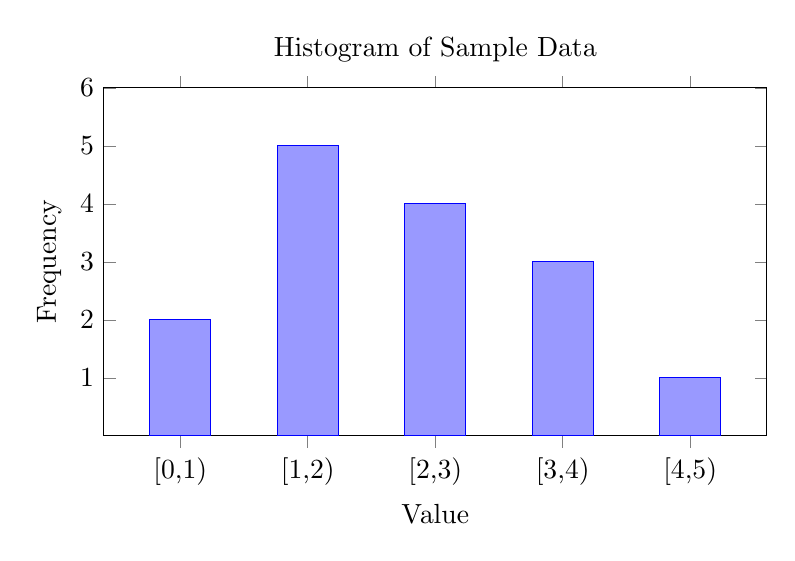
\begin{tikzpicture}
		\pgfplotsset{compat=1.18}
		\begin{axis}[
		    ybar,
		    ymin=0,
		    ymax=6,
		    bar width=22pt,
		    width=10cm,
		    height=6cm,
		    xlabel={Value},
		    ylabel={Frequency},
		    ytick={1,2,3,4,5,6},
		    xtick={1,2,3,4,5},
		    xticklabels={{[0,1)}, {[1,2)}, {[2,3)}, {[3,4)}, {[4,5)}},
		    enlarge x limits=0.15,
		    title={Histogram of Sample Data}
			]
		\addplot+[fill=blue!40] coordinates {(1,2) (2,5) (3,4) (4,3) (5,1)};
		\end{axis}
		\end{tikzpicture}
		\caption{A histogram representing the frequency of \glspl{datapoint} falling within discrete value ranges (i.e., bins). Each bar height shows the count of \glspl{sample} in the corresponding interval.}
		\label{fig:histogram}
		\end{figure}
		See also: \gls{dataset}, \gls{datapoint}, \gls{sample}.
	},
	first={histogram},
	text={histogram}  
}

\newglossaryentry{bootstrap}
{name={bootstrap},
	description={For\index{bootstrap} the analysis of \gls{ml} methods, it is often useful to interpret 
		a given set of \glspl{datapoint} $\dataset = \big\{ \datapoint^{(1)},\ldots,\datapoint^{(\samplesize)}\big\}$ 
		as \glspl{realization} of \gls{iid} \glspl{rv} with a common \gls{probdist} $p(\datapoint)$. In general, we 
		do not know $p(\datapoint)$ exactly, but we need to estimate it. The bootstrap uses the 
		\gls{histogram} of $\dataset$ as an estimator for the underlying \gls{probdist} $p(\datapoint)$. 
				\\
		See also: \gls{iid}, \gls{rv}, \gls{probdist}, \gls{histogram}.},
	first={bootstrap},
	text={bootstrap}  
}

\newglossaryentry{featurespace}
{name={feature space},
	description={The\index{feature space} \gls{feature} space of a given \gls{ml} application or method is 
		constituted by all potential values that the \gls{featurevec} of a \gls{datapoint} can 
		take on. A widely used choice for the \gls{feature} space is the \gls{euclidspace} $\mathbb{R}^{\featuredim}$, 
		with the dimension $\featurelen$ being the number of individual \glspl{feature} of a \gls{datapoint}.
				\\
		See also: \gls{feature}, \gls{ml}, \gls{featurevec}, \gls{datapoint}, \gls{feature}, \gls{euclidspace}.},
	first={feature space},
	text={feature space}  
}


\newglossaryentry{missingdata}
{name={missing data},
	description={Consider\index{missing data} a \gls{dataset} constituted by \glspl{datapoint} collected via 
		some physical \gls{device}. Due to imperfections and failures, some of the \gls{feature} 
		or \gls{label} values of \glspl{datapoint} might be corrupted or simply missing. 
		\Gls{data} imputation aims at estimating these missing values \cite{Abayomi2008DiagnosticsFM}. 
		We can interpret \gls{data} imputation as an \gls{ml} problem where the \gls{label} of a \gls{datapoint} is 
		the value of the corrupted \gls{feature}.
				\\
		See also: \gls{dataset}, \gls{datapoint}, \gls{device}, \gls{feature}, \gls{label}, \gls{data}, \gls{ml}. },
	first={missing data},
	text={missing data}  
}


\newglossaryentry{psd}
{name={positive semi-definite (psd)},
	description={A\index{positive semi-definite (psd)} (real-valued) symmetric matrix $\mQ = \mQ^{T} \in \mathbb{R}^{\featuredim \times \featuredim}$ 
	 	is referred to as psd if $\featurevec^{T} \mQ \featurevec \geq 0$ for every vector $\featurevec \in \mathbb{R}^{\featuredim}$. 
	 	The property of being psd can be extended from matrices to (real-valued) 
	 	symmetric \gls{kernel} \glspl{map} $\kernel: \featurespace \times \featurespace \rightarrow \mathbb{R}$ 
	 	(with $\kernel(\featurevec,\featurevec') = \kernel(\featurevec',\featurevec)$)
	 	as follows: For any finite set of \glspl{featurevec} $\featurevec^{(1)},\dots,\featurevec^{(\samplesize)}$, 
	 	the resulting matrix $\mQ \in \mathbb{R}^{\samplesize \times \samplesize}$ with 
		entries $Q_{\sampleidx,\sampleidx'} = \kernelmap{\featurevec^{(\sampleidx)}}{\featurevec^{(\sampleidx')}}$ 
		is psd \cite{LearningKernelsBook}.
			\\
		See also: \gls{kernel}, \gls{map}, \gls{featurevec}.},
	first={positive semi-definite (psd)},
	text={psd}  
}

\newglossaryentry{feature}
{name={feature}, plural={features},
	description={A\index{feature} feature of a \gls{datapoint} is one of its properties that can be 
		measured or computed easily without the need for human supervision. For example, if a \gls{datapoint} 
		is a digital image (e.g., stored as a \texttt{.jpeg} file), then we could use the red-green-blue intensities 
		of its pixels as features. Domain-specific synonyms for the term feature are "covariate," "explanatory variable," 
		"independent variable," "input (variable)," "predictor (variable)," or "regressor" \cite{Gujarati2021}, \cite{Dodge2003}, \cite{Everitt2022}. 
				\\
		See also: \gls{datapoint}.}, 
	first={feature},
	text={feature}  
}

\newglossaryentry{featurevec}
{name={feature vector}, plural={feature vectors},
	description={\Gls{feature} vector refers to a\index{feature vector} vector $\vx = \big(x_{1},\ldots,x_{\nrfeatures}\big)^{T}$ 
		whose entries are individual \glspl{feature} $x_{1},\ldots,x_{\nrfeatures}$. Many \gls{ml} methods 
		use \gls{feature} vectors that belong to some finite-dimensional \gls{euclidspace} $\mathbb{R}^{\nrfeatures}$. 
		For some \gls{ml} methods, however, it can be more convenient to work with \gls{feature} 
		vectors that belong to an infinite-dimensional \gls{vectorspace} (e.g., see \gls{kernelmethod}). 
			\\
		See also: \gls{feature}, \gls{ml}, \gls{euclidspace}, \gls{vectorspace}, \gls{kernelmethod}.}, 
	first={feature vector},
	text={feature vector}  
}


\newglossaryentry{label}
{name={label}, plural={labels},
	description={A\index{label} higher-level fact or quantity of interest associated with a \gls{datapoint}. 
		For example, if the \gls{datapoint} is an image, the label could indicate whether the 
		image contains a cat or not. Synonyms for label, commonly used in specific domains, 
		include "response variable," "output variable," and "target" \cite{Gujarati2021}, \cite{Dodge2003}, \cite{Everitt2022}.
				\\
		See also: \gls{datapoint}.},
	first={label},
	text={label}  
}


\newglossaryentry{data}
{name={data},
	 description={Data\index{data} refers to objects that carry information. These 
	 	objects can be either concrete physical objects (such as persons or animals) 
	 	or abstract concepts (such as numbers). We often use representations (or 
	 	approximations) of the original data that are more convenient for data processing. 
	 	These approximations use different mathematical structures such as relations 
		that are used in relational databases \cite{silberschatz2019database,codd1970relational}.
				\\
		See also: \gls{model}, \gls{dataset}, \gls{datapoint}.}, 
	text={data}
}

\newglossaryentry{dataset}
{name={dataset}, plural={datasets},
	description={A\index{dataset} dataset refers to a collection of \glspl{datapoint}. These 
		\glspl{datapoint} carry information about some quantity of interest (or \gls{label}) within 
		an \gls{ml} application. \gls{ml} methods use datasets for \gls{model} training (e.g., via \gls{erm})
		and \gls{model} \gls{validation}. Note that our notion of a dataset is very flexible, as 
		it allows for very different types of \glspl{datapoint}. Indeed, \glspl{datapoint} can be concrete 
		physical objects (such as humans or animals) or abstract objects (such as numbers). 
		As a case in point, Figure \ref{fig_cows_dataset_dict} depicts a dataset that consists of cows as 
		\glspl{datapoint}. 
		\begin{figure}[H]
				\begin{center}
		\label{fig:cowsintheswissalps_dict}
		\includegraphics[width=0.5\textwidth]{assets/CowsAustria.jpg}
		  \end{center}
		\caption{\label{fig_cows_dataset_dict}A cow herd somewhere in the Alps.}
	  \end{figure}
       Quite often, an \gls{ml} engineer does not have direct access to a dataset. Indeed, accessing the 
       dataset in Figure \ref{fig_cows_dataset_dict} would require us to visit the cow herd in the Alps. Instead, 
       we need to use an approximation (or representation) of the dataset which is more convenient 
       to work with. Different mathematical \glspl{model} have been developed for the representation (or approximation) 
       of datasets \cite{silberschatz2019database}, \cite{abiteboul1995foundations}, \cite{hoberman2009data}, \cite{ramakrishnan2002database}. 
       One of the most widely adopted data \gls{model} is the relational \gls{model}, which organizes \gls{data} 
       as a table (or relation) \cite{codd1970relational}, \cite{silberschatz2019database}.
		A table consists of rows and columns:
		\begin{itemize} 
		\item Each row of the table represents a single \gls{datapoint}.
		\item Each column of the table corresponds to a specific attribute of the \gls{datapoint}. 
		\gls{ml} methods can use attributes as \glspl{feature} and \glspl{label} of the \gls{datapoint}.
		\end{itemize}
		For example, Table \ref{tab:cowdata_dict} shows a representation of the dataset in Figure \ref{fig_cows_dataset_dict}. 
		In the relational \gls{model}, the order of rows is irrelevant, and each attribute (i.e., column) must be 
		precisely defined with a domain, which specifies the set of possible values. In \gls{ml} applications, 
		these attribute domains become the \gls{featurespace} and the \gls{labelspace}.
		\begin{table}[H]
			\centering
			\begin{tabular}{lcccc}
				\hline
				\textbf{Name} & \textbf{Weight} & \textbf{Age} & \textbf{Height} & \textbf{Stomach temperature} \\
				\hline
				Zenzi & 100 & 4 & 100 & 25 \\
				Berta & 140 & 3 & 130 & 23 \\
				Resi  & 120 & 4 & 120 & 31 \\
				\hline
			\end{tabular}
			\caption{A relation (or table) that represents the dataset in Figure \ref{fig_cows_dataset}.}
			\label{tab:cowdata_dict}
		\end{table}
 While the relational \gls{model} is useful for the study of many \gls{ml} applications, it may be 
 insufficient regarding the requirements for \gls{trustAI}. Modern 
 approaches like datasheets for datasets provide more comprehensive 
 documentation, including details about the \gls{data} collection process, intended 
 use, and other contextual information \cite{DatasheetData2021}.
 		\\
		See also: \gls{datapoint}, \gls{data}, \gls{feature}, \gls{featurespace}, \gls{labelspace}, \gls{trustAI}.},
 first={dataset},
 text={dataset}  
}

\newglossaryentry{predictor}
{name={predictor},
	description={A\index{predictor} predictor is a real-valued \gls{hypothesis} \gls{map}. 
		Given a \gls{datapoint} with \glspl{feature} $\featurevec$, the value 
		$\hypothesis(\featurevec) \in \mathbb{R}$ is used as a \gls{prediction} for the true 
		numeric \gls{label} $\truelabel \in \mathbb{R}$ of the \gls{datapoint}.
				\\
		See also: \gls{hypothesis}, \gls{map}, \gls{datapoint}, \gls{feature}, \gls{prediction}, \gls{label}. },
	first={predictor},
	text={predictor}  
}

\newglossaryentry{labeled datapoint}
{name={labeled datapoint}, plural={labeled datapoints},
 	description={A\index{labeled datapoint} \gls{datapoint} whose \gls{label} is known or has been determined 
 		by some means which might require human labor.
			\\
		See also: \gls{datapoint}, \gls{label}.},
 	first={labeled datapoint},
 	text={labeled datapoint}  
}

\newglossaryentry{rv}
{name={random variable (RV)}, plural={RVs},
 	description={An RV\index{random variable (RV)} is a \gls{function} that maps from 
 		a \gls{probspace} $\mathcal{P}$ to a value space \cite{BillingsleyProbMeasure}, \cite{GrayProbBook}. 
 		The \gls{probspace} consists of elementary events and is equipped with a \gls{probability} 
 		measure that assigns \glspl{probability} to subsets of $\mathcal{P}$. 
 		Different types of RVs include  
 		\begin{itemize} 
 			\item {binary RVs}, which map each elementary event to an element of a binary set (e.g., $\{-1,1\}$ or $\{\text{cat}, \text{no cat}\}$); 
 			\item {real-valued RVs}, which take values in the real numbers $\mathbb{R}$;  
 			\item {vector-valued RVs}, which map elementary events to the \gls{euclidspace} $\mathbb{R}^{\featuredim}$.  
 		\end{itemize} 
 		\Gls{probability} theory uses the concept of measurable spaces to rigorously define 
 		and study the properties of (large) collections of RVs \cite{BillingsleyProbMeasure}.
			\\
		See also: \gls{function}, \gls{probspace}, \gls{probability}, \gls{euclidspace}.}, 
	first={random variable (RV)},
	text={RV}  
}
 
 \newglossaryentry{probspace}
 {name={probability space}, 
 	description={A\index{probability space} \gls{probability} space is a mathematical 
 		\gls{model} of a physical process (i.e., a random experiment) with an uncertain outcome. 
 	   	Formally, a \gls{probability} space $\mathcal{P}$ is a triplet $(\Omega, \mathcal{F}, P)$ where
 		\begin{itemize} 
 		\item  $\Omega$ is a \gls{sample} space containing all possible elementary outcomes of a random experiment;
 		\item  $\mathcal{F}$ is a sigma-algebra, i.e., a collection of subsets of $\Omega$ (called events) that satisfies 
 		certain closure properties under set operations;
 		\item $P$ is a \gls{probability} measure, i.e., a \gls{function} that assigns a \gls{probability} $P(\mathcal{A}) \in [0,1]$ 
 		to each event $\mathcal{A} \in \mathcal{F}$. The \gls{function} must satisfy $P(\Omega) = 1$ and 	$
 		P\left(\bigcup_{i=1}^{\infty} \mathcal{A}_i\right) = \sum_{i=1}^{\infty} P(\mathcal{A}_i)$ for any 
 		countable sequence of pairwise disjoint events $\mathcal{A}_1, \mathcal{A}_2, \dots$ in $\mathcal{F}$.
 		\end{itemize}
 		\Gls{probability} spaces provide the foundation for defining \glspl{rv} and to reason about 
 		\gls{uncertainty} in \gls{ml} applications \cite{BillingsleyProbMeasure}, \cite{GrayProbBook}, \cite{ross2013first}.
				\\
		See also: \gls{probability}, \gls{model}, \gls{sample}, \gls{function}, \gls{rv}, \gls{uncertainty}, \gls{ml}.},  
 	first={probability space}, 
 	text={probability space}
 }
 
	
\newglossaryentry{realization}
{name={realization}, plural={realizations},
	description={Consider\index{realization} an \gls{rv} $x$ which maps each element 
		(i.e., outcome or elementary event) $\omega \in \mathcal{P}$ of a \gls{probspace} $\mathcal{P}$ 
		to an element $a$ of a measurable space $\mathcal{N}$ \cite{RudinBookPrinciplesMatheAnalysis}, \cite{BillingsleyProbMeasure}, \cite{HalmosMeasure}. 
		A realization of $x$ is any element $a' \in \mathcal{N}$ such that there is 
		an element $\omega' \in \mathcal{P}$ with $x(\omega') = a'$.
			\\
		See also: \gls{rv}, \gls{probspace}.}, 
	first={realization},
	text={realization}  
}

\newglossaryentry{trainset}
{name={training set}, plural={training sets},
	description={A\index{training set} training set is a \gls{dataset} $\dataset$ which consists of some \glspl{datapoint} used in \gls{erm} 
		to learn a \gls{hypothesis} $\learnthypothesis$. The average \gls{loss} of $\learnthypothesis$ on the 
		training set is referred to as the \gls{trainerr}. The comparison of the \gls{trainerr} with the 
		\gls{valerr} of $\learnthypothesis$ allows us to diagnose the \gls{ml} method and informs how to improve 
		the \gls{valerr} (e.g., using a different \gls{hypospace} or collecting more \glspl{datapoint}) \cite[Sec. 6.6]{MLBasics}.
			\\
		See also: \gls{dataset}, \gls{datapoint}, \gls{erm}, \gls{hypothesis}, \gls{loss}, \gls{trainerr}, \gls{valerr}, \gls{ml}, \gls{hypospace}.},
	first={training set},
	text={training set}  
}

\newglossaryentry{netmodel}
{name={networked model},
 	description={A\index{networked model} networked \gls{model} over an \gls{empgraph} $\graph = \pair{\nodes}{\edges}$ assigns 
   		a \gls{localmodel} (i.e., a \gls{hypospace}) to each node $\nodeidx \in \nodes$ of the \gls{empgraph} $\graph$.
   		\\
		See also: \gls{model}, \gls{empgraph}, \gls{localmodel}, \gls{hypospace}.}, 
   first={networked model},
   text={networked model}  
}

\newglossaryentry{batch}
{name={batch},
	description={In\index{batch} the context of \gls{stochGD}, a batch refers to a randomly 
		chosen subset of the overall \gls{trainset}. We use the \glspl{datapoint} in this subset 
		to estimate the \gls{gradient} of \gls{trainerr} and, in turn, to update the \gls{modelparams}.
			\\
		See also: \gls{stochGD}, \gls{trainset}, \gls{datapoint}, \gls{gradient}, \gls{trainerr}, \gls{modelparams}.}, 
 	first={batch},
 	firstplural={batches}, 
 	plural={batches}, 
 	text={batch}  
}

\newglossaryentry{netdata}
{name={networked data},
	description={Networked\index{networked data} \gls{data} consists of \glspl{localdataset} 
		that are related by some notion of pairwise similarity. We can represent networked 
		\gls{data} using a \gls{graph} whose nodes carry \glspl{localdataset} and edges encode 
		pairwise similarities. One example of networked \gls{data} arises in \gls{fl} applications 
		where \glspl{localdataset} are generated by spatially distributed \glspl{device}.
			\\
		See also: \gls{data}, \gls{localdataset}, \gls{graph}, \gls{fl}, \gls{device}.}, 
	first={networked data},
	text={networked data}  
}

\newglossaryentry{trainerr}
{name={training error},
	description={The\index{training error} average \gls{loss} of a \gls{hypothesis} when 
		predicting the \glspl{label} of the \glspl{datapoint} in a \gls{trainset}. 
		We sometimes refer by training error also to minimal average \gls{loss} 
		which is achieved by a solution of \gls{erm}.
				\\
		See also: \gls{loss}, \gls{hypothesis}, \gls{label}, \gls{datapoint}, \gls{trainset}, \gls{erm}.},
	first={training error},
	text={training error}  
}

\newglossaryentry{datapoint}
{name={data point}, plural={data points},
	description={A\index{data point} \gls{data} point is any object that conveys information \cite{coverthomas}. \Gls{data} points might be 
		students, radio signals, trees, forests, images, \glspl{rv}, real numbers, or proteins. We characterize \gls{data} points 
		using two types of properties. One type of property is referred to as a \gls{feature}. \Glspl{feature} are properties of a 
		\gls{data} point that can be measured or computed in an automated fashion. 
		A different kind of property is referred to as a \gls{label}. The \gls{label} of 
		a \gls{data} point represents some higher-level fact (or quantity of interest). In 
		contrast to \glspl{feature}, determining the \gls{label} of a \gls{data} point typically 
		requires human experts (or domain experts). Roughly speaking, \gls{ml} aims to predict 
		the \gls{label} of a \gls{data} point based solely on its \glspl{feature}. 
				\\
		See also: \gls{data}, \gls{rv}, \gls{feature}, \gls{label}, \gls{ml}.}, 
	first={data point},
	text={data point}  
}


\newglossaryentry{valerr}
{name={validation error}, plural={validation errors},
 	description={Consider\index{validation error} a \gls{hypothesis} $\learnthypothesis$ which is 
 		obtained by some \gls{ml} method, e.g., using \gls{erm} on a \gls{trainset}. The average \gls{loss} 
 		of $\learnthypothesis$ on a \gls{valset}, which is different from the \gls{trainset}, is referred 
 		to as the \gls{validation} error.
			\\
		See also: \gls{hypothesis}, \gls{ml}, \gls{erm}, \gls{trainset}, \gls{loss}, \gls{valset}, \gls{validation}.},
	first={validation error},
	text={validation error}  
}

\newglossaryentry{validation} 
{name={validation},
	description={Consider\index{validation} a \gls{hypothesis} $\learnthypothesis$ that has been 
		learned via some \gls{ml} method, e.g., by solving \gls{erm} on a \gls{trainset} $\dataset$. 
		Validation refers to the practice of evaluating the \gls{loss} incurred by the 
		\gls{hypothesis} $\learnthypothesis$ on a set of 
		\glspl{datapoint} that are not contained in the \gls{trainset} $\dataset$.
				\\
		See also: \gls{hypothesis}, \gls{ml}, \gls{erm}, \gls{trainset}, \gls{loss}, \gls{datapoint}. },
	first={validation},
	text={validation}  
}

\newglossaryentry{quadfunc}
{name={quadratic function},
	description={A\index{quadratic function} \gls{function} $f: \mathbb{R}^{\nrfeatures} \rightarrow \mathbb{R}$ of the form 
		$$f(\weights) =  \weights^{T} \mathbf{Q} \mathbf{w} + \mathbf{q}^{T} \weights+a,$$ with 
		some matrix $\mQ \in \mathbb{R}^{\nrfeatures \times \nrfeatures}$, vector $\vq \in \mathbb{R}^{\nrfeatures}$, 
		and scalar $a \in \mathbb{R}$.
		\\
		See also: \gls{function}. },
	first={quadratic function},
	text={quadratic function}  
}

\newglossaryentry{valset}
{name={validation set},
 	description={A\index{validation set} set of \glspl{datapoint} used to estimate 
  		the \gls{risk} of a \gls{hypothesis} $\learnthypothesis$ that has been learned by some 
  		\gls{ml} method (e.g., solving \gls{erm}). The average \gls{loss} of $\learnthypothesis$ 
  		on the \gls{validation} set is referred to as the \gls{valerr} and can be used to diagnose an 
  		\gls{ml} method (see \cite[Sec. 6.6]{MLBasics}). The comparison between \gls{trainerr} 
  		and \gls{valerr} can inform directions for the improvement of the \gls{ml} method (such as 
  		using a different \gls{hypospace}).
			\\
		See also: \gls{datapoint}, \gls{risk}, \gls{hypothesis}, \gls{ml}, \gls{erm}, \gls{loss}, \gls{validation}, \gls{valerr}, \gls{trainerr}, \gls{hypospace}.},
	first={validation set},
	text={validation set}  
}

\newglossaryentry{testset}
{name={test set},
	description={A\index{test set} set of \glspl{datapoint} that have  
		been used neither to train a \gls{model} (e.g., via \gls{erm}) nor in a \gls{valset} 
		to choose between different \glspl{model}.
				\\
		See also: \gls{datapoint}, \gls{model}, \gls{erm}, \gls{valset}.},
	first={test set},
	text={test set}  
}


\newglossaryentry{modelsel}
{name={model selection},
	description={In\index{model selection} \gls{ml}, \gls{model} selection refers to the 
		process of choosing between different candidate \glspl{model}. In its most 
		basic form, \gls{model} selection amounts to: 1) training each candidate \gls{model}; 
		2) computing the \gls{valerr} for each trained \gls{model}; and 3) choosing the \gls{model} 
		with the smallest \gls{valerr} \cite[Ch. 6]{MLBasics}. 
				\\
		See also: \gls{ml}, \gls{model}, \gls{valerr}.},
	first={model selection},
	text={model selection}  
}


\newglossaryentry{linclass}
{name={linear classifier}, 
	description={Consider\index{linear classifier} \glspl{datapoint} characterized by numeric \glspl{feature} $\featurevec \in \mathbb{R}^{\nrfeatures}$ 
	    	and a \gls{label} $\truelabel \in \labelspace$ from some finite \gls{labelspace} $\labelspace$. 
		A linear \gls{classifier} is characterized by having \glspl{decisionregion} that are 
		separated by hyperplanes in $\mathbb{R}^{\featuredim}$ \cite[Ch. 2]{MLBasics}.
				\\
		See also: \gls{datapoint}, \gls{feature}, \gls{label}, \gls{labelspace}, \gls{classifier}, \gls{decisionregion}.},
	first={linear classifier},
	text={linear classifier} 
}


\newglossaryentry{erm}
{name={empirical risk minimization (ERM)}, 
	description={ERM\index{empirical risk minimization (ERM)} is the \gls{optproblem} of finding 
		a \gls{hypothesis} (out of a \gls{model}) with the \gls{minimum} average \gls{loss} (or \gls{emprisk}) on a given \gls{dataset} 
		$\dataset$ (i.e., the \gls{trainset}). Many \gls{ml} methods are obtained from 
		\gls{emprisk} via specific design choices for the \gls{dataset}, \gls{model}, and \gls{loss} \cite[Ch. 3]{MLBasics}.
				\\
		See also: \gls{optproblem}, \gls{hypothesis}, \gls{model}, \gls{minimum}, \gls{loss}, \gls{emprisk}, \gls{dataset}, \gls{trainset}, \gls{ml}.},
	first={empirical risk minimization (ERM)},
	text={ERM} 
}


\newglossaryentry{multilabelclass}
{name={multi-label classification}, 
	description={Multi-\gls{label} 
		\gls{classification}\index{multi-label classification} problems and methods use \glspl{datapoint} 
		that are characterized by several \glspl{label}. As an example, consider a \gls{datapoint} 
		representing a picture with two \glspl{label}. One \gls{label} indicates the presence of a human 
		in this picture and another \gls{label} indicates the presence of a car.
				\\
		See also: \gls{label}, \gls{classification}, \gls{datapoint}.},
	    first={multi-label classification},
	    text={multi-label classification} 
}


\newglossaryentry{ssl}
{name={semi-supervised learning (SSL)}, 
	description={SSL\index{semi-supervised learning (SSL)} methods use unlabeled \glspl{datapoint}
		to support the learning of a \gls{hypothesis} from \glspl{labeled datapoint} \cite{SemiSupervisedBook}. 
		This approach is particularly useful for \gls{ml} applications that offer a large amount of 
		unlabeled \glspl{datapoint}, but only a limited number of \glspl{labeled datapoint}.
			\\
		See also: \gls{datapoint}, \gls{hypothesis}, \gls{labeled datapoint}, \gls{ml}.}, 
	first={semi-supervised learning (SSL)},
	text={SSL} 
}
	
	
\newglossaryentry{objfunc}
{name={objective function}, plural={objective functions}, 
	description={An\index{objective function} objective \gls{function} is a \gls{map} that assigns a numeric 
		objective value $f(\weights)$ to each choice $\weights$ of some variable that we want to 
		optimize (see Figure \ref{fig_obj_func_dict}). In the context of \gls{ml}, the optimization variable could 
		be the \gls{modelparams} of a \gls{hypothesis} $\hypothesis^{(\weights)}$. 
		Common objective \glspl{function} include the \gls{risk} (i.e., expected \gls{loss}) or the \gls{emprisk} 
		(i.e., average \gls{loss} over a \gls{trainset}). \gls{ml} methods apply optimization 
		techniques, such as \gls{gdmethods}, to find the choice $\weights$ with the 
		optimal value (e.g., the \gls{minimum} or the \gls{maximum}) of the objective \gls{function}.
		\\
		\begin{figure}[H]
			\begin{center}
			\begin{tikzpicture}[scale=1.0]
				% Axes
				\draw[->] (-0.5,0) -- (4.5,0) node[right] {$\weights$};
				\draw[->] (0,-0.5) -- (0,3.5);
				% Objective function curve
				\draw[thick,domain=0.3:4,smooth,variable=\x] 
				plot ({\x}, {0.5*(\x-2)^2 + 0.5});
				% Label the curve
				\node at (3.5,2.8) {$f(\weights)$};
			\end{tikzpicture} 
			\end{center}
		\caption{An objective \gls{function} maps each possible value $\weights$ of an optimization variable, such 
		as the \gls{modelparams} of an \gls{ml} \gls{model}, to a value that measures the usefulness 
	   of $\weights$.\label{fig_obj_func_dict}}
		\end{figure} 
		See also: \gls{function}, \gls{map}, \gls{ml}, \gls{modelparams}, \gls{hypothesis}, \gls{risk}, \gls{loss}, \gls{emprisk}, \gls{trainset}, \gls{gdmethods}, \gls{minimum}, \gls{maximum}, \gls{model}, \gls{lossfunc}.},
	first={objective function},
	text={objective function} 
}
	
\newglossaryentry{regularizer}
{name={regularizer}, 
	description={A regularizer\index{regularizer} 
		assigns each \gls{hypothesis} $\hypothesis$ from a \gls{hypospace} $\hypospace$ a quantitative 
		measure $\regularizer{\hypothesis}$ for how much its \gls{prediction} error on a \gls{trainset} might 
		differ from its \gls{prediction} errors on \glspl{datapoint} outside the \gls{trainset}. \Gls{ridgeregression} 
		uses the regularizer $\regularizer{\hypothesis} \defeq \normgeneric{\weights}{2}^{2}$ for linear \gls{hypothesis} 
		\glspl{map} $\hypothesis^{(\weights)}(\featurevec) \defeq \weights^{T} \featurevec$ \cite[Ch. 3]{MLBasics}. 
		\Gls{lasso} uses the regularizer $\regularizer{\hypothesis} \defeq \normgeneric{\weights}{1}$ 
		for linear \gls{hypothesis} \glspl{map} $\hypothesis^{(\weights)}(\featurevec) \defeq \weights^{T} \featurevec$ \cite[Ch. 3]{MLBasics}.
				\\
		See also: \gls{hypothesis}, \gls{hypospace}, \gls{prediction}, \gls{trainset}, \gls{datapoint}, \gls{ridgeregression}, \gls{map}, \gls{lasso}. },
	first={regularizer},
	text={regularizer} 
}


\newglossaryentry{regularization}
{name={regularization}, 
  description={A\index{regularization} key challenge of modern \gls{ml} applications 
  	    is that they often use large \glspl{model}, which have an \gls{effdim} in the order 
  	    of billions. Training a high-dimensional \gls{model} using basic \gls{erm}-based 
  	    methods is prone to \gls{overfitting}, i.e., the learned \gls{hypothesis} performs 
  	    well on the \gls{trainset} but poorly outside the \gls{trainset}. Regularization refers 
  	    to modifications of a given instance of \gls{erm} in order to avoid \gls{overfitting}, 
  	    i.e., to ensure that the learned \gls{hypothesis} performs not much worse outside 
  	    the \gls{trainset}. There are three routes for implementing regularization: 
		\begin{enumerate}[label=\arabic*)]
			\item {\Gls{model} pruning:} We prune the original \gls{model} $\hypospace$ to obtain a 
			smaller \gls{model} $\hypospace'$. For a parametric \gls{model}, the pruning can be 
			implemented via constraints on the \gls{modelparams} (such as $w_{1} \in [0.4,0.6]$ for 
			the weight of \gls{feature} $x_{1}$ in \gls{linreg}).
			\item {\Gls{loss} penalization:} We modify the \gls{objfunc} of \gls{erm} by adding a 
			penalty term to the \gls{trainerr}. The penalty term estimates how much larger the expected \gls{loss} (or \gls{risk}) 
			is compared to the average \gls{loss} on the \gls{trainset}. 
			\item {\Gls{dataaug}:} We can enlarge the \gls{trainset} $\dataset$ by adding 
			perturbed copies of the original \glspl{datapoint} in $\dataset$. One example for such 
			a perturbation is to add the \gls{realization} of an \gls{rv} to the \gls{featurevec} 
			of a \gls{datapoint}. 
		\end{enumerate} 
		Figure \ref{fig_equiv_dataaug_penal_dict} illustrates the above three routes to regularization. 
		These routes are closely related and sometimes fully equivalent. \Gls{dataaug} using \glspl{gaussrv} 
		to perturb the \glspl{featurevec} in the \gls{trainset} of \gls{linreg} 
		has the same effect as adding the penalty 
		$\lambda \normgeneric{\weights}{2}^2$ to the \gls{trainerr} (which is nothing but \gls{ridgeregression}). 
        		The decision on which route to use for regularization can be based on the 
        		available computational infrastructure. For example, it might be much easier to 
        		implement \gls{dataaug} than \gls{model} pruning. 
		\begin{figure}[H]
			\begin{center} 
				\begin{tikzpicture}[scale = 1]
					% Axes
					\draw[->, very thick] (0,0.5) -- (7.7,0.5) node[right] {\gls{feature} $\feature$};       % X-axis
					\draw[->, very thick] (0.5,0) -- (0.5,4.2) node[above] {\gls{label} $\truelabel$};   % Y-axis
					\draw[color=black, thick, dashed, domain = -1: 6.2, variable = \x]  plot ({\x},{\x*0.4 + 2.0}) ;     
					\draw[color=black, thick, dashed, domain = -1: 6.2, variable = \x]  plot ({\x},{\x*0.6 + 2.0}) ;     
					% Add a lasso around the two dashed lines
	          			% Ellipse around the two dashed lines
					\draw[blue, thick] (5, 4.5) ellipse [x radius=0.2cm, y radius=1cm];
					\node at (5, 5.8) [text=black, font=\small] {$\{ \hypothesis: \hypothesis(x)\!=\!w_{1}x\!+\!w_{0}; w_{1} \in [0.4,0.6]\}$};
					\node at (6.7,4.5) {$\hypothesis(\feature)$};    
					\coordinate (l1)   at (1.2, 2.48);
					\coordinate (l2) at (1.4, 2.56);
					\coordinate (l3)   at (1.7,  2.68);
					\coordinate (l4)   at (2.2, 2.2*0.4+2.0);
					\coordinate (l5) at (2.4, 2.4*0.4+2.0);
					\coordinate (l6)   at (2.7,  2.7*0.4+2.0);
					\coordinate (l7)   at (3.9,  3.9*0.4+2.0);
					\coordinate (l8) at (4.2, 4.2*0.4+2.0);
					\coordinate (l9)   at (4.5,  4.5*0.4+2.0);
					\coordinate (n1)   at (1.2, 1.8);
					\coordinate (n2) at (1.4, 1.8);
					\coordinate (n3)   at (1.7,  1.8);
					\coordinate (n4)   at (2.2, 3.8);
					\coordinate (n5) at (2.4, 3.8);
					\coordinate (n6)   at (2.7,  3.8);
					% augemented data point obtained by perturbing feature, not touching label value 
					\coordinate (n7)   at (3.9, 2.6);
					\coordinate (n8) at (4.2, 2.6);
					\coordinate (n9)   at (4.5,  2.6);
					\node at (n1)  [circle,draw,fill=red,minimum size=6pt,scale=0.6, name=c1] {};
					\node at (n2)  [circle,draw,fill=blue,minimum size=6pt, scale=0.6, name=c2] {};
					\node at (n3)  [circle,draw,fill=red,minimum size=6pt,scale=0.6,  name=c3] {};
					\node at (n4)  [circle,draw,fill=red,minimum size=12pt, scale=0.6, name=c4] {};  
					\node at (n5)  [circle,draw,fill=blue,minimum size=12pt,scale=0.6,  name=c5] {};
					\node at (n6)  [circle,draw,fill=red,minimum size=12pt, scale=0.6, name=c6] {};  
					\node at (n7)  [circle,draw,fill=red,minimum size=12pt,scale=0.6,  name=c7] {};
					\node at (n8)  [circle,draw,fill=blue,minimum size=12pt, scale=0.6, name=c8] {};
					\node at (n9)  [circle,draw,fill=red,minimum size=12pt, scale=0.6, name=c9] {};
					\draw [<->] ($ (n7) + (0,-0.3) $)  --  ($ (n9) + (0,-0.3) $) node [pos=0.4, below] {$\sqrt{\regparam}$}; ; 
					\draw[<->, color=red, thick] (l1) -- (c1);  
					\draw[<->, color=blue, thick] (l2) -- (c2);  
					\draw[<->, color=red, thick] (l3) -- (c3);  
					\draw[<->, color=red, thick] (l4) -- (c4);  
					\draw[<->, color=blue, thick] (l5) -- (c5);  
					\draw[<->, color=red, thick] (l6) -- (c6);  
					\draw[<->, color=red, thick] (l7) -- (c7);  
					\draw[<->, color=blue, thick] (l8) -- (c8);  
					\draw[<->, color=red, thick] (l9) -- (c9);  
					\draw[fill=blue] (6.2, 3.7)  circle (0.1cm) node [black,xshift=2.3cm] {original \gls{trainset} $\dataset$};
					\draw[fill=red] (6.2, 3.2)  circle (0.1cm) node [black,xshift=1.3cm] {augmented};
					\node at (4.6,1.2)  [minimum size=12pt, font=\fontsize{12}{0}\selectfont, text=blue] {$\frac{1}{\samplesize} \sum_{\sampleidx=1}^\samplesize \lossfunc{\pair{\featurevec^{(\sampleidx)}}{ \truelabel^{(\sampleidx)}}}{\hypothesis}$};
					\node at (7.8,1.2)  [minimum size=12pt, font=\fontsize{12}{0}\selectfont, text=red] {$+\regparam \regularizer{\hypothesis}$};
				\end{tikzpicture}
				\caption{Three approaches to regularization: 1) \gls{dataaug}; 2) \gls{loss} penalization; and 3) \gls{model} 
				pruning (via constraints on \gls{modelparams}). \label{fig_equiv_dataaug_penal_dict} }
			\end{center}
		\end{figure} 
		See also: \gls{overfitting}, \gls{dataaug}, \gls{validation}, \gls{modelsel}.
		},
	first={regularization},
	text={regularization} 
}
	

\newglossaryentry{rerm}
{name={regularized empirical risk minimization (RERM)}, 
	description={Basic \gls{erm} learns a \gls{hypothesis} (or trains a \gls{model}) $\hypothesis \in \hypospace$ 
		based solely on the \gls{emprisk} $\emprisk{\hypothesis}{\dataset}$ incurred on a \gls{trainset} $\dataset$. 
		To make \gls{erm} less prone to \gls{overfitting}, we can implement \gls{regularization} by 
		including a (scaled) \gls{regularizer} $\regularizer{\hypothesis}$ in the learning objective. 
		This leads to RERM\index{regularized empirical risk minimization (RERM)} such that
		\begin{equation}
			\label{equ_def_rerm_dict}
			\learnthypothesis \in \argmin_{\hypothesis \in \hypospace} \emprisk{\hypothesis}{\dataset} + \regparam \regularizer{\hypothesis}.
		\end{equation}
		The \gls{parameter} $\regparam \geq 0$ controls the \gls{regularization} strength. 
		For $\regparam = 0$, we recover standard \gls{erm} without \gls{regularization}. As $\regparam$ increases, the 
		learned \gls{hypothesis} is increasingly biased toward small values of $\regularizer{\hypothesis}$. 
		The component $\regparam \regularizer{\hypothesis}$ in the \gls{objfunc} of \eqref{equ_def_rerm_dict} 
		can be intuitively understood as a surrogate for the increased average \gls{loss} that may 
		occur when predicting \glspl{label} for \glspl{datapoint} outside the \gls{trainset}. This intuition  
		can be made precise in various ways. For example, consider a \gls{linmodel} trained using \gls{sqerrloss} 
		and the \gls{regularizer} $\regularizer{\hypothesis} = \normgeneric{\weights}{2}^{2}$. 
		In this setting, $\regparam \regularizer{\hypothesis}$ corresponds to the expected increase in \gls{loss} 
		caused by adding \glspl{gaussrv} to the \glspl{featurevec} in the \gls{trainset} 
		\cite[Ch. 3]{MLBasics}.
		A principled construction for the \gls{regularizer} $\regularizer{\hypothesis}$ 
		arises from approximate upper bounds on the \gls{generalization} error. The resulting 
		RERM instance is known as \gls{srm} \cite[Sec. 7.2]{ShalevShwartz2009}.
				\\
		See also: \gls{erm}, \gls{hypothesis}, \gls{model}, \gls{emprisk}, \gls{trainset}, \gls{overfitting}, \gls{regularization}, \gls{regularizer}, \gls{parameter}, \gls{objfunc}, \gls{loss}, \gls{label}, \gls{datapoint}, \gls{linmodel}, \gls{sqerrloss}, \gls{gaussrv}, \gls{featurevec}, \gls{generalization}, \gls{srm}.}, 
	first={regularized empirical risk minimization (RERM)},
	text={RERM} 
}


\newglossaryentry{generalization}
{name={generalization}, 
	description={Generalization\index{generalization} refers to the ability of a \gls{model} trained on a \gls{trainset} to make accurate 
		\glspl{prediction} on new, unseen \glspl{datapoint}. This is a central goal of \gls{ml} and \gls{ai}, i.e., 
		to learn patterns that extend beyond the \gls{trainset}. Most \gls{ml} systems 
		use \gls{erm} to learn a \gls{hypothesis} $\learnthypothesis \in \hypospace$ by minimizing 
		the average \gls{loss} over a \gls{trainset} of \glspl{datapoint} $\datapoint^{(1)}, \ldots, \datapoint^{(\samplesize)}$, 
		which is denoted $\trainset$. However, success on the \gls{trainset} does not guarantee success on 
		unseen \gls{data}—this discrepancy is the challenge of generalization. \\ To study generalization 
		mathematically, we need to formalize the notion of ``unseen'' \gls{data}. A widely used 
		approach is to assume a \gls{probmodel} for \gls{data} generation, such as the \gls{iidasspt}. 
		Here, we interpret \glspl{datapoint} as independent \glspl{rv} with an identical 
		\gls{probdist} $p(\datapoint)$. This \gls{probdist}, which is assumed fixed but unknown, 
		allows us to define the \gls{risk} of a trained \gls{model} $\learnthypothesis$ as the expected \gls{loss}
		\[
		\risk{\learnthypothesis}=\expect_{\datapoint \sim p(\datapoint)} \big\{ \loss(\learnthypothesis, \datapoint) \big\}.
		\]
		The difference between \gls{risk} $\risk{\learnthypothesis}$ and \gls{emprisk} $\emprisk{\learnthypothesis}{\trainset}$ 
		is known as the \gls{gengap}. Tools from \gls{probability} theory, such as \glspl{concentrationinequ} 
		and uniform convergence, allow us to bound this gap under certain conditions \cite{ShalevMLBook}.\\
		Generalization without \gls{probability}: \Gls{probability} theory is one way to study how well a 
		\gls{model} generalizes beyond the \gls{trainset}, but it is not the only way. Another option is to use 
		simple, deterministic changes to the \glspl{datapoint} in the \gls{trainset}. The basic idea is that a 
		good \gls{model} $\learnthypothesis$ should be robust, i.e., its \gls{prediction} $\learnthypothesis(\featurevec)$ 
		should not change much if we slightly change the \glspl{feature} $\featurevec$ of a \gls{datapoint} $\datapoint$. 
		\\[1mm] For example, an object detector trained on smartphone photos should still detect the object if a few 
		random pixels are masked \cite{OnePixelAttack}. Similarly, it should deliver the same result if we rotate 
		the object in the image \cite{MallatUnderstandingDeepLearning}.
		  \begin{figure}[H]
		                   	\centering
		                   	\begin{tikzpicture}[scale=0.8]
							   \draw[lightblue, fill=lightblue, opacity=0.5] (3, 2) ellipse (6cm and 2cm);
								\node[black] at (6, 3) {$p(\datapoint)$};
		                   		\fill[blue] (1, 3) circle (4pt) node[below, xshift=0pt, yshift=0pt] {$\datapoint^{(1)}$};
		                   		\fill[blue] (5, 1) circle (4pt) node[below] {$\datapoint^{(2)}$};
		                   		\fill[blue] (1.6, 3) circle (3pt);
		                   		\fill[blue] (0.4, 3) circle (3pt);
		                   		\draw[<->, thin] (1, 3) -- (1.6, 3);
		                   		\draw[<->, thin] (1, 3) -- (0.4, 3);
		                   		\fill[blue] (5.6, 1) circle (3pt);
		                   		\fill[blue] (4.4, 1) circle (3pt);
		                   		\draw[<->, thin] (5, 1) -- (5.6, 1);
		                   		\draw[<->, thin] (5, 1) -- (4.4, 1);
		                   		\draw[black, thick, domain=0:6, smooth] plot (\x, {- 1*\x + 5});
		                   		\node[black] at (3, 2.5) [right] {$\learnthypothesis$};
		                   	\end{tikzpicture}
		                   	\caption{Two \glspl{datapoint} $\datapoint^{(1)},\datapoint^{(2)}$ that are used as a \gls{trainset} 
		                   		to learn a \gls{hypothesis} $\learnthypothesis$ via \gls{erm}. We can evaluate $\learnthypothesis$ 
		                   		outside $\trainset$ either by an \gls{iidasspt} with some underlying \gls{probdist} $p(\datapoint)$ 
		                   		or by perturbing the \glspl{datapoint}.}
		                   	\label{fig:polynomial_fit_dict}
		                   \end{figure}
		See also: \gls{model}, \gls{trainset}, \gls{prediction}, \gls{datapoint}, \gls{ml}, \gls{ai}, \gls{erm}, \gls{hypothesis}, \gls{loss}, \gls{data}, \gls{probmodel}, \gls{iidasspt}, \gls{rv}, \gls{probdist}, \gls{risk}, \gls{emprisk}, \gls{gengap}, \gls{probability}, \gls{concentrationinequ}, \gls{feature}.},
	first={generalization},
	text={generalization} 
}

\newglossaryentry{gengap}
{name={generalization gap}, 
	description={The difference\index{generalization gap} between the performance of a trained \gls{model} on the 
		\gls{trainset} $\trainset$ and its performance on \glspl{datapoint} outside of $\trainset$. We can make this notion 
		precise by using a \gls{probmodel} that allows to compute the \gls{risk} of a trained \gls{model} as the expected 
		\gls{loss}. However, the \gls{probdist} underlying this expectation is typically unknown and needs to be somehow 
		estimated. \Gls{validation} techniques use different constructions of a \gls{valset}, which is different from 
		the \gls{trainset},  to estimate the generalization gap.  
		\\
		See also: \gls{generalization}, \gls{erm}, \gls{lossfunc}, \gls{validation}.}, 
	first={generalization gap}, 
	text={generalization gap}
} 
	
\newglossaryentry{concentrationinequ}
{name={concentration inequality}, 
	description={An upper bound on the \gls{probability}\index{concentration inequality} that an \gls{rv} deviates 
		more than a prescribed amount from its \gls{expectation} \cite{Wain2019}. 
		\\
		See also: \gls{probability}, \gls{rv}, \gls{expectation}.}, 
	first={concentration inequality},
	firstplural={concentration inequalities},
	plural={concentration inequalities},  
	text={concentration inequality}
}


\newglossaryentry{boosting}
{name={boosting}, 
	description={Boosting\index{boosting} is an iterative \gls{optmethod} to learn an accurate 
		\gls{hypothesis} \gls{map} (or strong learner) by sequentially combining less accurate 
		\gls{hypothesis} \glspl{map} (referred to as weak learners) \cite[Ch. 10]{hastie01statisticallearning}.
		For example, weak learners are shallow \glspl{decisiontree} which are combined to 
		obtain a deep \gls{decisiontree}. Boosting can be understood as a \gls{generalization} 
		of \gls{gdmethods} for \gls{erm} using parametric \glspl{model} and \gls{smooth} \glspl{lossfunc} 
		\cite{Friedman2001}. Just like \gls{gd} iteratively updates \gls{modelparams} to reduce the \gls{emprisk}, 
		boosting iteratively combines (e.g., by summation) \gls{hypothesis} \glspl{map} to reduce the \gls{emprisk}. 
		A widely-used instance of the generic boosting idea is referred to as \gls{gradient} boosting, which 
		uses \glspl{gradient} of the \gls{lossfunc} for combining the weak learners \cite{Friedman2001}. 
		\begin{figure}[H]
			\begin{center}
				\begin{tikzpicture}[scale=1.2]
					% Axes
					\draw[->] (-0.5,0) -- (5.5,0) node[right] {$\hypothesis$};
					\draw[->] (0,-0.5) -- (0,4.5) node[above] {$\lossfunc{\vz}{\hypothesis}$};
					\draw[thick,domain=0.2:5,smooth,variable=\x,blue!60] plot ({\x},{(4 - 1.3*\x + 0.15*\x*\x)});
					\foreach \x/\label in {0.7/$\hypothesis^{(0)}$, 1.5/$\hypothesis^{(1)}$, 2.3/$\hypothesis^{(2)}$, 3.0/$\hypothesis^{(3)}$} {
						\draw[dashed, gray] (\x, 0) -- (\x, {4 - 1.3*\x + 0.15*\x*\x}); % helper line
						\filldraw[black] (\x, {4 - 1.3*\x + 0.15*\x*\x}) circle (2pt);   % point
						\node[below] at (\x, -0.1) {\label};                             % label
					}
				\end{tikzpicture}
			\end{center} 
			\caption{Boosting methods construct a sequence of \gls{hypothesis} \glspl{map} $\hypothesis^{(0)},\hypothesis^{(1)},\ldots$ 
				            that are increasingly strong learners (i.e., incurring a smaller \gls{loss}).}
     		\end{figure} 
     		See also: \gls{optmethod}, \gls{hypothesis}, \gls{map}, \gls{decisiontree}, \gls{generalization}, \gls{gdmethods}, \gls{erm}, \gls{model}, \gls{smooth}, \gls{lossfunc}, \gls{gd}, \gls{modelparams}, \gls{emprisk}, \gls{gradient}, \gls{loss}, \gls{gradstep}.}, 
	first={boosting}, 
	text={boosting}
} 

	
\newglossaryentry{gtv}
{name={generalized total variation (GTV)}, 
	description={GTV is a\index{generalized total variation (GTV)} 
		measure of the variation of trained \glspl{localmodel} $\localhypothesis{\nodeidx}$ 
		(or their \gls{modelparams} $\localparams{\nodeidx}$) assigned to the nodes $\nodeidx=1,\ldots,\nrnodes$ 
		of an undirected weighted \gls{graph} $\graph$ with edges $\edges$. Given a measure $\discrepancy{\hypothesis}{\hypothesis'}$ 
		for the \gls{discrepancy} between \gls{hypothesis} \glspl{map} $\hypothesis,\hypothesis'$, the GTV is 
		\begin{equation} 
			\nonumber
			\sum_{\edge{\nodeidx}{\nodeidx'}\in \edges} \edgeweight_{\nodeidx,\nodeidx'} 
			\discrepancy{\localhypothesis{\nodeidx}}{\localhypothesis{\nodeidx'}}.
		\end{equation}
		Here, $\edgeweight_{\nodeidx,\nodeidx'}>0$ denotes the weight of the undirected edge $\edge{\nodeidx}{\nodeidx'}\in \edges$.
				\\
		See also: \gls{localmodel}, \gls{modelparams}, \gls{graph}, \gls{discrepancy}, \gls{hypothesis}, \gls{map}.},
	first={GTV},
	text={GTV} 
}
	
\newglossaryentry{srm}
{name={structural risk minimization (SRM)}, 
	description={SRM\index{structural risk minimization (SRM)} is an
		instance of \gls{rerm}, with which the \gls{model} $\hypospace$ can be expressed 
		as a countable union of submodels such that $\hypospace = \bigcup_{n=1}^{\infty} \hypospace^{(n)}$. 
		Each submodel $\hypospace^{(n)}$ permits the derivation of an approximate upper bound 
		on the \gls{generalization} error incurred when applying \gls{erm} to train $\hypospace^{(n)}$. 
		These individual bounds—one for each submodel—are then combined to form a \gls{regularizer} 
		used in the \gls{rerm} objective. 
        		These approximate upper bounds (one for each $\hypospace^{(n)}$) are then combined 
		to construct a \gls{regularizer} for \gls{rerm} \cite[Sec.\ 7.2]{ShalevMLBook}.
				\\
		See also: \gls{rerm}, \gls{model}, \gls{generalization}, \gls{erm}, \gls{regularizer}, \gls{risk}.},
	first={structural risk minimization (SRM)},
	text={SRM}
 }

 \newglossaryentry{rlm}
 {name={regularized loss minimization (RLM)},
 	description={See\index{regularized loss minimization (RLM)} \gls{rerm}.},
 	text={RLM}
 }
 

\newglossaryentry{datapoisoning}
{name={data poisoning}, 
  description={\Gls{data}\index{data poisoning} poisoning refers to the intentional manipulation 
  	(or fabrication) of \glspl{datapoint} to steer the training of an \gls{ml} \gls{model} \cite{Liu2021}, \cite{PoisonGAN}. 
  	\Gls{data} poisoning \glspl{attack} take various forms, including:
  	\begin{itemize}
  		\item \Gls{backdoor} \glspl{attack} : implanting triggers into training \gls{data} so that the trained \gls{model} 
  		behaves normally on typical \glspl{featurevec} but misclassifies a \gls{featurevec} with a trigger pattern.
  		\item \gls{dosattack}: degrading overall performance of the trained \gls{model} by injecting mislabeled or 
  		adversarial examples to prevent effective learning.
  	\end{itemize}
	\Gls{data} poisoning is particularly concerning in decentralized or distributed \gls{ml} settings (such as \gls{fl}), 
	where training \gls{data} cannot be centrally verified.
				\\
		See also: \gls{backdoor}, \gls{attack}, \gls{dosattack}, \gls{trustAI}.},
	first={data poisoning},
	text={data poisoning} 
}
	
	
\newglossaryentry{backdoor}
{name={backdoor}, 
	description={A\index{backdoor} backdoor attack refers 
		to the intentional manipulation of the training process underlying an \gls{ml} method. This manipulation 
		can be implemented by perturbing the \gls{trainset} (i.e., through \gls{datapoisoning}) or via the 
		optimization \gls{algorithm} used by an \gls{erm}-based method. The goal of a 
		backdoor attack is to nudge the learned \gls{hypothesis} $\learnthypothesis$ 
		towards specific \glspl{prediction} for a certain range of \gls{feature} values. This range of \gls{feature} 
		values serves as a key (or trigger) to unlock a backdoor in the sense of 
		delivering anomalous \glspl{prediction}. The key $\featurevec$ and the corresponding 
		anomalous \gls{prediction} $\learnthypothesis(\featurevec)$ are only known to the attacker.
				\\
		See also: \gls{ml}, \gls{trainset}, \gls{datapoisoning}, \gls{algorithm}, \gls{erm}, \gls{hypothesis}, \gls{prediction}, \gls{feature}.},
	first={backdoor},
	text={backdoor} 
}


\newglossaryentry{clustasspt}
{name={clustering assumption}, 
 description={The\index{clustering assumption} \gls{clustering} assumption postulates that 
 	\glspl{datapoint} in a \gls{dataset} form a (small) number of groups or \glspl{cluster}. 
 	\Glspl{datapoint} in the same \gls{cluster} are more similar to each 
		other than those outside the \gls{cluster} \cite{SemiSupervisedBook}. We obtain different 
		\gls{clustering} methods by using different notions of similarity between \glspl{datapoint}.
				\\
		See also: \gls{clustering}, \gls{datapoint}, \gls{dataset}, \gls{cluster}.},
		first={clustering assumption},
		text={clustering assumption} }

	
\newglossaryentry{dosattack}
{name={denial-of-service attack}, plural={denial-of-service attacks},
	description={A\index{denial-of-service attack} 
		denial-of-service attack aims (e.g., via \gls{datapoisoning}) to steer the training of a \gls{model} 
		such that it performs poorly for typical \glspl{datapoint}.
				\\
		See also: \gls{datapoisoning}, \gls{model}, \gls{datapoint}.},
	first={denial-of-service attack},
	text={denial-of-service attack} 
}

\newglossaryentry{netexpfam}
{name={networked exponential families (nExpFam)}, 
	description={A\index{networked exponential families (nExpFam)} collection of exponential 
		families, each of them assigned to a node of an \gls{empgraph}. The \gls{modelparams} are coupled 
	   	via the network structure by requiring them to have a small \gls{gtv} \cite{JungNetExp2020}.
	   		\\
		See also: \gls{empgraph}, \gls{modelparams}, \gls{gtv}.},
	first={networked exponential family (nExpFam)},
	text={nExpFam} 
}
	 

\newglossaryentry{scatterplot}
{name={scatterplot}, 
	description={A\index{scatterplot} 
		visualization technique that depicts \glspl{datapoint} by markers in a two-dimensional plane. 
		Figure \ref{fig_scatterplot_temp_FMI_dict} depicts an example of a scatterplot.  
		\begin{figure}[H]
			\begin{center}
				\begin{tikzpicture}[scale=1]
					\tikzset{x=2cm,y=2cm,every path/.style={>=latex},node style/.style={circle,draw}}
					\begin{axis}[axis x line=none,
						axis y line=none,
						ylabel near ticks,
						xlabel near ticks,
						enlarge y limits=true,
						xmin=-5, xmax=30,
						ymin=-5, ymax=30,
						width=6cm, height=6cm ]
						\addplot[only marks] table [x=mintmp, y=maxtmp, col sep = semicolon] {assets/FMIData1.csv};
						\node at (axis cs:26,2) [anchor=west] {$\feature$};
						\node at (axis cs:0,30) [anchor=west] {$\truelabel$};
						\draw[->] (axis cs:-5,0) -- (axis cs:30,0);
						\draw[->] (axis cs:0,-5) -- (axis cs:0,30);
					\end{axis}
				\end{tikzpicture}
				\vspace*{-10mm}
			\end{center}
			\caption{A scatterplot with circle markers, where the \glspl{datapoint} represent daily weather conditions in Finland. 
				Each \gls{datapoint} is characterized by its \gls{minimum} daytime temperature $\feature$ 
				as the \gls{feature} and its \gls{maximum} daytime temperature $\truelabel$ as the \gls{label}. 
				The temperatures have been measured at the \gls{fmi} weather station Helsinki Kaisaniemi 
				during 1.9.2024 - 28.10.2024.}
			\label{fig_scatterplot_temp_FMI_dict}
			\vspace*{-3mm}
			\end{figure}
		A scatterplot can enable the visual inspection of \glspl{datapoint} that are naturally 
		represented by \glspl{featurevec} in high-dimensional spaces.
		\\
		See also: \gls{datapoint}, \gls{minimum}, \gls{feature}, \gls{maximum}, \gls{label}, \gls{fmi}, \gls{featurevec}, \gls{dimred}.},
	first={scatterplot},
	text={scatterplot} 
}


\newglossaryentry{stepsize}
{name={step size}, 
	description={See\index{step size} \gls{learnrate}.}, 
	first={step size},
	text={step size} 
}

\newglossaryentry{learnrate}
{name={learning rate}, 
	description={Consider\index{learning rate} 
		an iterative \gls{ml} method for finding or learning a useful \gls{hypothesis} $\hypothesis \in \hypospace$. 
		Such an iterative method repeats similar computational (update) steps that adjust or 
		modify the current \gls{hypothesis} to obtain an improved \gls{hypothesis}. One 
		well-known example of such an iterative learning method is \gls{gd} and its variants, \gls{stochGD} and 
		\gls{projgd}. A key \gls{parameter} of an iterative method is the learning rate. 
		The learning rate controls the extent to which the current \gls{hypothesis} 
		can be modified during a single iteration. A well-known example of such a \gls{parameter} 
		is the \gls{stepsize} used in \gls{gd} \cite[Ch. 5]{MLBasics}.
				\\
		See also: \gls{ml}, \gls{hypothesis}, \gls{gd}, \gls{stochGD}, \gls{projgd}, \gls{parameter}, \gls{stepsize}.},
	first={learning rate},
	text={learning rate} 
}

\newglossaryentry{featuremap}
{name={feature map}, 
	description={\Gls{feature} \gls{map} refers to a\index{feature map} \gls{map} 
		that transforms the original \glspl{feature} of a \gls{datapoint} into new \glspl{feature}. The 
		so-obtained new \glspl{feature} might be preferable over the original \glspl{feature} for 
		several reasons. For example, the arrangement of \glspl{datapoint} might become 
		simpler (or more linear) in the new \gls{featurespace}, allowing the use of \glspl{linmodel} 
		in the new \glspl{feature}. This idea is a main driver for the development of \glspl{kernelmethod} \cite{LearningKernelsBook}. 
		Moreover, the hidden layers of a \gls{deepnet} can be interpreted as a trainable \gls{feature} \gls{map} 
		followed by a \gls{linmodel} in the form of the output layer. Another reason for learning a \gls{feature} \gls{map}
		could be that learning a small number of new \glspl{feature} helps to avoid \gls{overfitting} and 
		ensures \gls{interpretability} \cite{Ribeiro2016}. The special case of a \gls{feature} \gls{map} delivering 
		two numeric \glspl{feature} is particularly useful for \gls{data} visualization. Indeed, we can depict 
		\glspl{datapoint} in a \gls{scatterplot} by using two \glspl{feature} as the coordinates of a \gls{datapoint}.
				\\
		See also: \gls{feature}, \gls{map}, \gls{datapoint}, \gls{featurespace}, \gls{linmodel}, \gls{kernelmethod}, \gls{deepnet}, \gls{overfitting}, \gls{interpretability}, \gls{data}, \gls{scatterplot}.},
	first={feature map},
	text={feature map} 
}
	
 
 \newglossaryentry{lasso}
 {name={least absolute shrinkage and selection operator (Lasso)}, 
	description={The Lasso\index{least absolute shrinkage and selection operator (Lasso)} is an 
		instance of \gls{srm}. It learns the \gls{weights} $\weights$ of a \gls{linearmap} 
		$\hypothesis(\featurevec) = \weights^{T} \featurevec$ based on a \gls{trainset}. 
		Lasso is obtained from \gls{linreg} by adding the scaled $\ell_{1}$-\gls{norm} 
		$\regparam \normgeneric{\weights}{1}$ to the average \gls{sqerrloss} incurred on the \gls{trainset}. 
				\\
		See also: \gls{srm}, \gls{weights}, \gls{linearmap}, \gls{trainset}, \gls{linreg}, \gls{norm}, \gls{sqerrloss}.},
	first={Lasso},
	text={Lasso} 
}
 
 \newglossaryentry{simgraph}
 {name={similarity graph}, 
 	description={Some\index{similarity graph} \gls{ml} applications generate \glspl{datapoint} that 
 		are related by a domain-specific notion of similarity. These similarities can be 
 		represented conveniently using a similarity \gls{graph} $\graph = \big(\nodes \defeq \{1,\ldots,\samplesize\},\edges\big)$. 
 		The node $\sampleidx \in \nodes$ represents the $\sampleidx$-th \gls{datapoint}. Two 
 		nodes are connected by an undirected edge if the corresponding \glspl{datapoint} are similar. 
				\\
		See also: \gls{ml}, \gls{datapoint}, \gls{graph}.},
 	first={similarity graph},
	text={similarity graph} 
}
 
 
 \newglossaryentry{kld}
 {name={Kullback-Leibler divergence (KL divergence)}, 
 	description={The\index{Kullback-Leibler divergence (KL divergence)} KL divergence is a quantitative 
 		 measure of how much one \gls{probdist} is different from another \gls{probdist} \cite{coverthomas}.  
		 		\\
		See also: \gls{probdist}.},
 	first={Kullback-Leibler divergence (KL divergence)},
	text={KL divergence} 
}

\newglossaryentry{LapMat}
{name={Laplacian matrix},
	description={The\index{Laplacian matrix} structure of a \gls{graph} $\graph$, with 
		nodes $\nodeidx=1,\ldots,\nrnodes$, can be analyzed using the properties of 
		special matrices that are associated with $\graph$. One such matrix is the 
		\gls{graph} Laplacian matrix $\mL^{(\graph)} \in \mathbb{R}^{\nrnodes \times \nrnodes}$, 
		which is defined for an undirected and weighted \gls{graph} \cite{Luxburg2007}, \cite{Ng2001}. 
		It is defined element-wise as (see Figure \ref{fig_lap_mtx_dict})
	\begin{equation}
		\LapMatEntry{\graph}{\nodeidx}{\nodeidx'} \defeq \begin{cases} - \edgeweight_{\nodeidx,\nodeidx'} & \mbox{ for } \nodeidx\neq \nodeidx', \edge{\nodeidx}{\nodeidx'}\!\in\!\edges, \\ 
			\sum_{\nodeidx'' \neq \nodeidx} \edgeweight_{\nodeidx,\nodeidx''} & \mbox{ for } \nodeidx = \nodeidx', \\ 
							0 & \mbox{ else.} \end{cases}
	 \end{equation}
  		Here, $\edgeweight_{\nodeidx,\nodeidx'}$ denotes the \gls{edgeweight} of an edge $\edge{\nodeidx}{\nodeidx'} \in \edges$. 
  	\begin{figure}[H]
  	\begin{center}
   	\begin{minipage}{0.45\textwidth}
	\begin{tikzpicture}
%	 				% 		% Left part - Graph
	 	 		\begin{scope}[every node/.style={circle, draw, minimum size=1cm}]
	 					 			\node (1) at (0,0) {1};
	 					 			\node (2) [below left=of 1] {2};
	 					 			\node (3) [below right=of 1] {3};
	 					 		   \draw (1) -- (2);
	 					 			\draw (1) -- (3);
	 					 		\end{scope}
	 				 	\end{tikzpicture}
	 			 	\end{minipage} 
	 			 	\hspace*{-15mm}
 		 		\begin{minipage}{0.45\textwidth}
	 			 	 \begin{equation} 
	 				 		 \LapMat{\graph} = \begin{pmatrix} 2 & -1& -1 \\ -1& 1 & 0 \\  -1 & 0 & 1 \end{pmatrix}  
	 				 		 \nonumber
	 				 		 \end{equation} 
	 			 \end{minipage}
	 	 \caption{\label{fig_lap_mtx_dict} Left: Some undirected \gls{graph} $\graph$ with three nodes $\nodeidx=1,2,3$. 
	 		 	Right: The Laplacian matrix $\LapMat{\graph}  \in \mathbb{R}^{3 \times 3}$ of $\graph$.} 
	 		 	\end{center}
	 \end{figure}
		See also: \gls{graph}, \gls{edgeweight}.},
	first={Laplacian matrix},
	text={Laplacian matrix}
}

\newglossaryentry{algconn}
{name={algebraic connectivity},
	description={The\index{algebraic connectivity} algebraic connectivity of an undirected \gls{graph} 
		is the second-smallest \gls{eigenvalue} $\eigval{2}$ of its \gls{LapMat}. A \gls{graph} is connected if and only if 
		$\eigval{2} >0$. 
				\\
		See also: \gls{graph}, \gls{eigenvalue}, \gls{LapMat}.},
	first={algebraic connectivity},
	text={algebraic connectivity}
}


\newglossaryentry{cfwmaxmin}
{name ={Courant–Fischer–Weyl min-max characterization}, 
	description={Consider\index{Courant–Fischer–Weyl min-max characterization} a \gls{psd} 
	matrix $\mQ \in \mathbb{R}^{\nrfeatures \times \nrfeatures}$ with 
	\gls{evd} (or spectral decomposition), 
	$$ \mQ = \sum_{\featureidx=1}^{\nrfeatures} \eigval{\featureidx} \vu^{(\featureidx)} \big(  \vu^{(\featureidx)}  \big)^{T}.$$ 
	Here, we use the ordered (in increasing fashion) \glspl{eigenvalue} 
	\begin{equation}
		\nonumber
		 \eigval{1}  \leq  \ldots \leq \eigval{\nrnodes}. 
	\end{equation}
	The Courant–Fischer–Weyl min-max characterization \cite[Th. 8.1.2]{GolubVanLoanBook} 
	represents the \glspl{eigenvalue} of $\mQ$ as the solutions to certain \glspl{optproblem}.
			\\
		See also: \gls{psd}, \gls{evd}, \gls{eigenvalue}, \gls{optproblem}.}, 
	first={Courant–Fischer–Weyl min-max characterization (CFW)}, 
	text={CFW}
}

\newglossaryentry{kernel}
{name={kernel}, 
	description={Consider\index{kernel} \glspl{datapoint} characterized by a \gls{featurevec} $\featurevec \in \featurespace$ 
		with a generic \gls{featurespace} $\featurespace$. A (real-valued) kernel $\kernel: \featurespace \times \featurespace \rightarrow \mathbb{R}$ 
		assigns each pair of \glspl{featurevec} $\featurevec, \featurevec' \in \featurespace$ a real number $\kernelmap{\featurevec}{\featurevec'}$. 
		The value $\kernelmap{\featurevec}{\featurevec'}$ is often interpreted as a measure for the similarity between $\featurevec$ 
		and $\featurevec'$. \Glspl{kernelmethod} use a kernel to transform the \gls{featurevec} $\featurevec$ to a new \gls{featurevec} $\vz = \kernelmap{\featurevec}{\cdot}$. 
         	This new \gls{featurevec} belongs to a linear \gls{featurespace} $\featurespace'$ which is (in general)  
          	different from the original \gls{featurespace} $\featurespace$. The \gls{featurespace} $\featurespace'$ has 
          	a specific mathematical structure, i.e., it is a reproducing kernel \gls{hilbertspace} \cite{LearningKernelsBook}, \cite{LampertNowKernel}.
          		\\
		See also: \gls{featurevec}, \gls{featurespace}, \gls{kernelmethod}, \gls{hilbertspace}.
          },
	first={kernel},text={kernel} }
	
\newglossaryentry{kernelmethod}
{name={kernel method}, 
	plural={kernel methods}, 
	description={A\index{kernel method} \gls{kernel} method is an \gls{ml} method that uses a 
	\gls{kernel} $\kernel$ to map the original (i.e., raw) \gls{featurevec} $\featurevec$ of a 
	\gls{datapoint} to a new (transformed) \gls{featurevec} $\vz = \kernelmap{\featurevec}{\cdot}$ \cite{LearningKernelsBook}, \cite{LampertNowKernel}.
	The motivation for transforming the \glspl{featurevec} is that, by using a suitable \gls{kernel}, 
	the \glspl{datapoint} have a "more pleasant" geometry in the transformed \gls{featurespace}. 
	For example, in a binary \gls{classification} problem, using transformed \glspl{featurevec} $\vz$ might 
	allow us to use \glspl{linmodel}, even if the \glspl{datapoint} are not linearly 
	separable in the original \gls{featurespace} (see Figure \ref{fig_linsep_kernel_dict}). 
	\begin{figure}[H]
\begin{center}
 \begin{tikzpicture}[auto,scale=0.6]
        % Left rectangle (\featurespace)
       % \draw [thick] (-9,-3) rectangle (-2,4) node [anchor=east,above] {$\featurespace$};
        \draw [thick] (-6,2) circle (0.1cm) node[anchor=west] {\hspace*{0mm}$\featurevec^{(5)}$};
       \draw [thick] (-8,1.6) circle (0.1cm) node[anchor=west] {\hspace*{0mm}$\featurevec^{(4)}$};
        \draw [thick] (-7.4,-1.7) circle (0.1cm) node[anchor=west] {\hspace*{0mm}$\featurevec^{(3)}$};
        \draw [thick] (-6,-1.9) circle (0.1cm) node[anchor=west] {\hspace*{0mm}$\featurevec^{(2)}$};
        \draw [thick] (-6.5,0.0) rectangle ++(0.1cm,0.1cm) node[anchor=west,above] {\hspace*{0mm}$\featurevec^{(1)}$};
%
%        % Right rectangle (\featurespace')
      % \draw [thick] (0,-4) rectangle (7,3) node [anchor=east,above] {$\featurespace'$};
        \draw [thick] (4,0) circle (0.1cm) node[anchor=north] {\hspace*{0mm}$\vz^{(5)}$};
        \draw [thick] (5,0) circle (0.1cm) node[anchor=north] {\hspace*{0mm}$\vz^{(4)}$};
        \draw [thick] (6,0) circle (0.1cm) node[anchor=north] {\hspace*{0mm}$\vz^{(3)}$};
        \draw [thick] (7,0) circle (0.1cm) node[anchor=north] {\hspace*{0mm}$\vz^{(2)}$};
        \draw [thick] (2,0) rectangle ++(0.1cm,0.1cm) node[anchor=west,above] {\hspace*{0mm}$\vz^{(1)}$};
%
%        % Arrow from left rectangle to right rectangle
       \draw[->,bend left=30] (-3,0) to node[midway,above] {$\vz = \kernelmap{\featurevec}{\cdot}$} (1,0);
    \end{tikzpicture}
\end{center}
\caption{
Five \glspl{datapoint} characterized by \glspl{featurevec} $\featurevec^{(\sampleidx)}$ 
and \glspl{label} $\truelabel^{(\sampleidx)} \in \{ \circ, \square \}$, for $\sampleidx=1,\ldots,5$. 
With these \glspl{featurevec}, there is no way to separate the two classes 
by a straight line (representing the \gls{decisionboundary} of a \gls{linclass}). 
In contrast, the transformed \glspl{featurevec} $\vz^{(\sampleidx)} = \kernelmap{\featurevec^{(\sampleidx)}}{\cdot}$ 
allow us to separate the \glspl{datapoint} using a \gls{linclass}.  \label{fig_linsep_kernel_dict}}
\end{figure}
		See also: \gls{kernel}, \gls{featurevec}, \gls{featurespace}, \gls{linclass}.},
	first={kernel method},
	text={kernel method} 
}

	

\newglossaryentry{cm}
{name={confusion matrix}, 
 description={Consider\index{confusion matrix} \glspl{datapoint}, which are characterized 
		by \glspl{feature} $\featurevec$ and \gls{label} $\truelabel$, having values from the finite 
		\gls{labelspace} $\labelspace = \{1,\ldots,\nrcluster\}$. For a given \gls{hypothesis} $\hypothesis$, 
		the confusion matrix is a $\nrcluster \times \nrcluster$ matrix with rows representing the elements of 
		$\labelspace$. The columns of a confusion matrix correspond to the \gls{prediction} $\hypothesis(\featurevec)$. 
		The $(\clusteridx,\clusteridx')$-th entry of the confusion matrix is the fraction of 
		\glspl{datapoint} with \gls{label} $\truelabel\!=\! \clusteridx$ and resulting in a \gls{prediction} $\hypothesis(\featurevec)\!=\!\clusteridx'$.
				\\
		See also: \gls{label}, \gls{labelspace}, \gls{hypothesis}, \gls{classification}.},
	first={confusion matrix},text={confusion matrix} }


\newglossaryentry{featuremtx}
{name={feature matrix}, 
	description={Consider\index{feature matrix} a \gls{dataset} $\dataset$ 
		with $\samplesize$ \glspl{datapoint} with \glspl{featurevec} $\featurevec^{(1)},\ldots,\featurevec^{(\samplesize)} \in \mathbb{R}^{\nrfeatures}$. It is convenient to 
		collect the individual \glspl{featurevec} into a \gls{feature} 
		matrix $\mX \defeq \big(\featurevec^{(1)},\ldots,\featurevec^{(\samplesize)}\big)^{T}$ 
		of size $\samplesize \times \nrfeatures$.
				\\
		See also: \gls{dataset}, \gls{datapoint}, \gls{featurevec}, \gls{feature}.},
	first={feature matrix},
	text={feature matrix} 
}

\newglossaryentry{dbscan}
{name={density-based spatial clustering of applications with noise (DBSCAN)}, 
	description={DBSCAN\index{density-based spatial clustering of applications with 
			noise (DBSCAN)} refers to a \gls{clustering} \gls{algorithm} for \glspl{datapoint} 
			that are characterized by numeric \glspl{featurevec}. 
		Like \gls{kmeans} and \gls{softclustering} via \gls{gmm}, also DBSCAN uses the Euclidean 
		distances between \glspl{featurevec} to determine the \glspl{cluster}. However, in contrast to \gls{kmeans} 
		and \gls{gmm}, DBSCAN uses a different notion of similarity between \glspl{datapoint}. 
		DBSCAN considers two \glspl{datapoint} as similar if they are connected 
		via a sequence (i.e., path) of close-by intermediate \glspl{datapoint}. 
		Thus, DBSCAN might consider two \glspl{datapoint} as similar (and therefore belonging 
		to the same \gls{cluster}) even if their \glspl{featurevec} have a large Euclidean distance.
				\\
		See also: \gls{clustering}, \gls{graph}, \gls{kmeans}, \gls{gmm}, \gls{cluster}.},
	first={density-based spatial clustering of applications with noise (DBSCAN)},
	text={DBSCAN} 
}

\newglossaryentry{fl}
{name={federated learning (FL)}, 
	description={FL\index{federated learning (FL)} 
		is an umbrella term for \gls{ml} methods that train \glspl{model} in a collaborative 
		fashion using decentralized \gls{data} and computation.
				\\
		See also: \gls{ml}, \gls{model}, \gls{data}.},
	first={federated learning (FL)},
	text={FL} 
}
	
\newglossaryentry{cfl}
{name={clustered federated learning (CFL)}, 
 description={CFL\index{clustered federated learning (CFL)} trains \glspl{localmodel} for the 
 	\glspl{device} in a \gls{fl} application by using a \gls{clustasspt}, i.e., the \glspl{device} 
 	of an \gls{empgraph} form \glspl{cluster}. Two \glspl{device} in the same \gls{cluster} generate 
 	\glspl{localdataset} with similar statistical properties. CFL pools the \glspl{localdataset} of \glspl{device} 
 	in the same \gls{cluster} to obtain a \gls{trainset} for a \gls{cluster}-specific \gls{model}. 
 	\Gls{gtvmin} clusters \glspl{device} implicitly by enforcing approximate similarity of \gls{modelparams} 
 	across well-connected nodes of the \gls{empgraph}.\\ 
 	See also: \gls{fl}, \gls{clustasspt}, \gls{empgraph}, \gls{cluster}, \gls{graphclustering}.},
	first={clustered federated learning (CFL)},
	text={CFL} 
}

\newglossaryentry{iid}
{name={independent and identically distributed (i.i.d.)}, 
	description={It\index{independent and identically distributed (i.i.d.)} can be useful to 
		interpret \glspl{datapoint} $\datapoint^{(1)},\ldots,\datapoint^{(\samplesize)}$ 
		as \glspl{realization} of i.i.d. \glspl{rv} with 
		a common \gls{probdist}. If these \glspl{rv} are continuous-valued, their joint \gls{pdf} 
		is $p\big(\datapoint^{(1)},\ldots,\datapoint^{(\samplesize)} \big) = \prod_{\sampleidx=1}^{\samplesize} p \big(\datapoint^{(\sampleidx)}\big)$, 
		with $p(\datapoint)$ being the common 
		marginal \gls{pdf} of the underlying \glspl{rv}.
				\\
		See also: \gls{datapoint}, \gls{realization}, \gls{rv}, \gls{probdist}, \gls{pdf}.},
	first={independent and identically distributed (i.i.d.)},
	text={{i.i.d.}} 
}


\newglossaryentry{outlier}
{name={outlier}, 
	description={Many\index{outlier} \gls{ml} methods 
		are motivated by the \gls{iidasspt}, which interprets \glspl{datapoint} as \glspl{realization} of 
		\gls{iid} \glspl{rv} with a common \gls{probdist}. The \gls{iidasspt} is useful for applications  
		where the statistical properties of the \gls{data} generation process are stationary (or time-invariant) \cite{Brockwell91}. 
		However, in some applications the \gls{data} consists of a majority of regular \glspl{datapoint} 
		that conform with an \gls{iidasspt} as well as a small number of \glspl{datapoint} that have fundamentally different 
       		statistical properties compared to the regular \glspl{datapoint}. We refer to a \gls{datapoint} that 
        		substantially deviates from the statistical properties of most \glspl{datapoint} as an 
        		outlier. Different methods for outlier detection use different measures for this deviation. 
        		Statistical learning theory studies fundamental limits on the ability to mitigate outliers reliably \cite{doi:10.1137/0222052}, \cite{10.1214/20-AOS1961}.
        		\\
		See also: \gls{ml}, \gls{iidasspt}, \gls{datapoint}, \gls{realization}, \gls{iid}, \gls{rv}, \gls{probdist}, \gls{data}.},
	 first={outlier},
	 text={outlier} 
}

\newglossaryentry{decisionregion}
{name={decision region}, plural={decision regions}, 
	description={Consider\index{decision region} 
		a \gls{hypothesis} \gls{map} $\hypothesis$ that delivers values from a finite set $\labelspace$. 
		For each \gls{label} value (i.e., category) $a \in \labelspace$, the \gls{hypothesis} $\hypothesis$ 
		determines a subset of \gls{feature} values $\featurevec \in \featurespace$ that result 
		in the same output $\hypothesis(\featurevec)=a$. We refer to this subset as a decision 
		region of the \gls{hypothesis} $\hypothesis$.
				\\
		See also: \gls{hypothesis}, \gls{map}, \gls{label}, \gls{feature}.},
	first={decision region},
	text={decision region} 
}


\newglossaryentry{decisionboundary}
{name={decision boundary}, 
	description={Consider\index{decision boundary} a 
		\gls{hypothesis} \gls{map} $\hypothesis$ that reads in a \gls{feature} vector 
		$\featurevec \in \mathbb{R}^{\featuredim}$ and delivers a value from a finite set $\labelspace$. 
		The decision boundary of $\hypothesis$ is the set of vectors $\featurevec \in \mathbb{R}^{\featuredim}$ 
		that lie between different \glspl{decisionregion}. More precisely, a 
		vector $\featurevec$ belongs to the decision boundary if and only 
		if each \gls{neighborhood} $\{ \featurevec': \| \featurevec - \featurevec' \| \leq \varepsilon \}$, 
		for any $\varepsilon >0$, contains at least two vectors with different \gls{function} values.
				\\
		See also: \gls{hypothesis}, \gls{map}, \gls{feature}, \gls{decisionregion}, \gls{neighborhood}, \gls{function}.},
	first={decision boundary},
	text={decision boundary} 
}


\newglossaryentry{euclidspace}
{name={Euclidean space}, 
	description={The\index{Euclidean space} 
		Euclidean space $\mathbb{R}^{\featuredim}$ of dimension $\featuredim \in \mathbb{N}$ consists 
		of vectors $\featurevec= \big(\feature_{1},\ldots,\feature_{\featurelen}\big)$, with $\featuredim$ 
		real-valued entries $\feature_{1},\ldots,\feature_{\featuredim} \in \mathbb{R}$. Such an Euclidean 
		space is equipped with a geometric structure defined by the inner product 
		$\featurevec^{T} \featurevec' = \sum_{\featureidx=1}^{\featuredim} \feature_{\featureidx} \feature'_{\featureidx}$ 
		between any two vectors $\featurevec,\featurevec' \in \mathbb{R}^{\featuredim}$ \cite{RudinBookPrinciplesMatheAnalysis}.},
	first={Euclidean space},
	text={Euclidean space} 
}

\newglossaryentry{eerm}
{name={explainable empirical risk minimization (EERM)}, 
	description={EERM is an\index{explainable empirical risk minimization (EERM)} 
		instance of \gls{srm} that adds a \gls{regularization} term to the 
		average \gls{loss} in the \gls{objfunc} of \gls{erm}. 
		The \gls{regularization} term is chosen to favor \gls{hypothesis} \glspl{map} that are intrinsically 
		explainable for a specific user. This user is characterized by their \glspl{prediction} provided 
		for the \glspl{datapoint} in a \gls{trainset} \cite{Zhang:2024aa}.
				\\
		See also: \gls{srm}, \gls{regularization}, \gls{loss}, \gls{objfunc}, \gls{erm}, \gls{hypothesis}, \gls{map}, \gls{prediction}, \gls{datapoint}, \gls{trainset}.},
	first={explainable empirical risk minimization (EERM)},
	text={EERM} 
}
	
	
\newglossaryentry{kmeans}
{name={$k$-means}, 
	description={The\index{$k$-means} $k$-\glspl{mean} \gls{algorithm} 
		is a \gls{hardclustering} method which assigns each \gls{datapoint} of a \gls{dataset} 
		to precisely one of $k$ different \glspl{cluster}. The method alternates between updating 
		the \gls{cluster} assignments (to the \gls{cluster} with the nearest \gls{mean}) and, given the 
		updated \gls{cluster} assignments, re-calculating the \gls{cluster} \glspl{mean} \cite[Ch. 8]{MLBasics}.
				\\
		See also: \gls{mean}, \gls{algorithm}, \gls{hardclustering}, \gls{datapoint}, \gls{dataset}, \gls{cluster}.},
	first={$k$-means},
	text={$k$-means} 
}


\newglossaryentry{xml}
{name={explainable machine learning (XML)}, 
	description={XML\index{explainable machine learning (XML)} 
		methods aim at complementing each \gls{prediction} with an \gls{explanation} of 
		how the \gls{prediction} has been obtained. The construction of an explicit \gls{explanation} 
		might not be necessary if the \gls{ml} method uses a sufficiently simple (or interpretable) \gls{model} \cite{rudin2019stop}.
				\\
		See also: \gls{prediction}, \gls{explanation}, \gls{ml}, \gls{model}.},
	first={XML},
	text={XML} 
}

\newglossaryentry{fmi}
{name={Finnish Meteorological Institute (FMI)}, 
	description={The\index{Finnish Meteorological Institute (FMI)}
		FMI is a government agency responsible for gathering 
		and reporting weather \gls{data} in Finland.
				\\
		See also: \gls{data}.},
	first={Finnish Meteorological Institute (FMI)},
	text={FMI} 
}
	
	
\newglossaryentry{samplemean}
{name={sample mean}, 
	description={The\index{sample mean} \gls{sample} \gls{mean} 
		$\vm \in \mathbb{R}^{\nrfeatures}$ for a given \gls{dataset}, with \glspl{featurevec} $\featurevec^{(1)},\ldots,\featurevec^{(\samplesize)} \in \mathbb{R}^{\nrfeatures}$, 
		is defined as 
		$$\vm = (1/\samplesize) \sum_{\sampleidx=1}^{\samplesize} \featurevec^{(\sampleidx)}.$$ 
					\\
		See also: \gls{sample}, \gls{mean}, \gls{dataset}, \gls{featurevec}.},
	first={sample mean},
	text={sample mean} 
}

	
\newglossaryentry{samplecovmtx}
{name={sample covariance matrix}, 
	description={The\index{sample covariance matrix} 
		\gls{sample} \gls{covmtx} $\widehat{\bf \Sigma} \in \mathbb{R}^{\nrfeatures \times \nrfeatures}$ 
		for a given set of \glspl{featurevec} $\featurevec^{(1)},\ldots,\featurevec^{(\samplesize)} \in \mathbb{R}^{\nrfeatures}$ is defined as 
		$$\widehat{\bf \Sigma} = (1/\samplesize) \sum_{\sampleidx=1}^{\samplesize} (\featurevec^{(\sampleidx)}\!-\!\widehat{\vm}) (\featurevec^{(\sampleidx)}\!-\!\widehat{\vm})^{T}.$$ 
		Here, we use the \gls{samplemean} $\widehat{\vm}$. 
				\\
		See also: \gls{sample}, \gls{covmtx}, \gls{featurevec}, \gls{samplemean}.},
	first={sample covariance matrix},
	text={sample covariance matrix} 
}

\newglossaryentry{covmtx}
{name={covariance matrix}, 
	description={The\index{covariance matrix} covariance matrix of an \gls{rv} $\vx \in \mathbb{R}^{\featuredim}$ 
		is defined as $\expect \bigg \{ \big( \vx - \expect \big\{ \vx \big\} \big)  \big(\vx - \expect \big\{ \vx \big\} \big)^{T} \bigg\}$.
				\\
		See also: \gls{rv}.},
	first={covariance matrix},
	text={covariance matrix} 
}
	
\newglossaryentry{highdimregime}
{name={high-dimensional regime}, 
 description={The\index{high-dimensional regime} 
		high-dimensional regime of \gls{erm} is characterized by the \gls{effdim} of the \gls{model} 
		being larger than the \gls{samplesize}, i.e., the number of (labeled) \glspl{datapoint} in the \gls{trainset}. 
		For example, \gls{linreg} methods operate in the high-dimensional regime whenever the number $\featuredim$ of \glspl{feature} 
		used to characterize \glspl{datapoint} exceeds the number of \glspl{datapoint} in the \gls{trainset}. 
		Another example of \gls{ml} methods that operate in the high-dimensional regime is large \glspl{ann}, which have 
		far more tunable \gls{weights} (and bias terms) than the total number of \glspl{datapoint} in the \gls{trainset}. 
		High-dimensional statistics is a recent main thread of \gls{probability} theory that studies the 
		behavior of \gls{ml} methods in the high-dimensional regime \cite{Wain2019}, \cite{BuhlGeerBook}.
				\\
		See also: \gls{erm}, \gls{effdim}, \gls{overfitting}, \gls{regularization}.},
   first={high-dimensional regime},
   text={high-dimensional regime} 
}

\newglossaryentry{covariance}
{name={covariance}, 
 description={The\index{covariance} covariance between two real-valued 
 	\glspl{rv} $x$ and $y$, defined on a common \gls{probspace}, measures their linear 
 	dependence. It defined as 
			$$
			\cov{x}{y} = \expect\big\{ \big(x - \expect\{ x\} \big)\big(y - \expect\{y\} \big)\big\}.
			$$
	A positive covariance indicates that $x$ and $y$ tend to increase together, 
	while a negative covariance suggests that one tends to increase as the other decreases. 
	If $\cov{x}{y} = 0$, the \glspl{rv} are said to be uncorrelated, though not necessarily statistically 
	independent. See Figure \ref{fig:covariance-examples_dict} for visual illustrations.
		\begin{figure}
		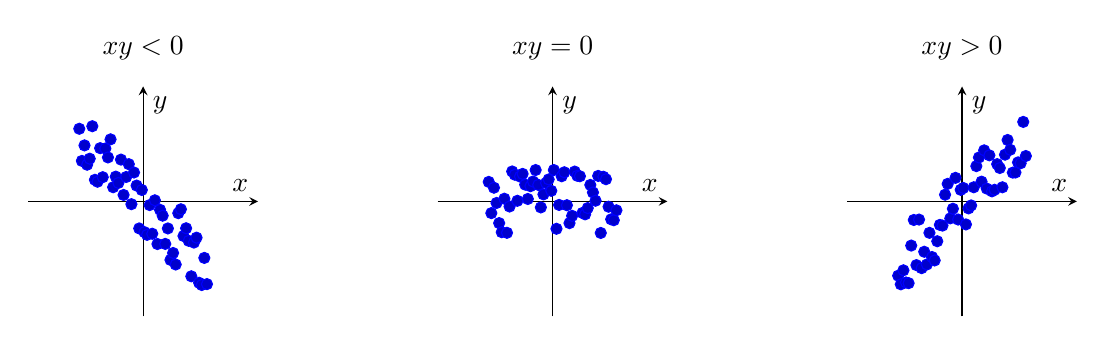
\begin{tikzpicture}
		 % Negative covariance
		\begin{scope}[shift={(0,0)}]
			\begin{axis}[
				width=4.5cm, height=4.5cm,
						 title={$\cov{x}{y} <0$},
				xlabel={$x$}, ylabel={$y$},
				xmin=-3, xmax=3, ymin=-3, ymax=3,
				xtick=\empty, ytick=\empty,
				axis lines=middle, enlargelimits
				]
				\addplot+[only marks, mark=*, samples=50, domain=-2:2] 
				({x}, {-x + rand});
			\end{axis}
		\end{scope}
		% Zero covariance
		\begin{scope}[shift={(5.2cm,0)}]
			\begin{axis}[
				width=4.5cm, height=4.5cm,
				 title={$\cov{x}{y} =0$}, xlabel={$x$}, ylabel={$y$},
				xmin=-3, xmax=3, ymin=-3, ymax=3,
				xtick=\empty, ytick=\empty,
				axis lines=middle, enlargelimits
				]
				\addplot+[only marks, mark=*, samples=50, domain=-2:2] 
				({x}, {rand});
			\end{axis}
		\end{scope}
		% Positive covariance
		\begin{scope}[shift={(10.4cm,0)}]
			\begin{axis}[
				width=4.5cm, height=4.5cm,
				 title={$\cov{x}{y} > 0$},
				xlabel={$x$}, ylabel={$y$},
				xmin=-3, xmax=3, ymin=-3, ymax=3,
				xtick=\empty, ytick=\empty,
				axis lines=middle, enlargelimits
				]
				\addplot+[only marks, mark=*, samples=50, domain=-2:2] 
				({x}, {x + rand});
			\end{axis}
		\end{scope}
		\end{tikzpicture}
			\caption{\Glspl{scatterplot} illustrating \glspl{realization} from three different \glspl{probmodel} for two 
				\glspl{rv} with different covariance values: negative (left), zero (center), and positive (right).}
			\label{fig:covariance-examples_dict}
		\end{figure}
		},
	first={covariance},
	text={covariance} 
}

\newglossaryentry{gmm}
{name={Gaussian mixture model (GMM)}, 
	description={A GMM\index{Gaussian mixture model (GMM)} 
		is a particular type of \gls{probmodel} for a numeric vector $\featurevec$ (e.g., 
		the \glspl{feature} of a \gls{datapoint}). Within a GMM, the vector $\featurevec$ is drawn from a randomly 
		selected \gls{mvndist} $p^{(\clusteridx)} = \mvnormal{\meanvec{\clusteridx}}{\covmtx{\clusteridx}}$ with 
		$\clusteridx = I$. The index $I \in \{1,\ldots,\nrcluster\}$ is an \gls{rv} with \glspl{probability} $\prob{I=\clusteridx} = p_{\clusteridx}$.
	     	Note that a GMM is parametrized by the \gls{probability} $p_{\clusteridx}$, the 
		\gls{mean} vector $\clustermean^{(\clusteridx)}$, and the \gls{covmtx} $\mathbf{C}^{(\clusteridx)}$ for each $\clusteridx=1,\ldots,\nrcluster$. 
		GMMs are widely used for \gls{clustering}, density estimation, and as a generative \gls{model}. 
				\\
		See also: \gls{probmodel}, \gls{feature}, \gls{datapoint}, \gls{mvndist}, \gls{rv}, \gls{mean}, \gls{covmtx}, \gls{clustering}, \gls{model}.},
	first={Gaussian mixture model (GMM)},
	text={GMM} 
}
 
\newglossaryentry{maxlikelihood}
{name={maximum likelihood}, 
 description={Consider\index{maximum likelihood} \glspl{datapoint} $\dataset=\big\{ \datapoint^{(1)}, \ldots, \datapoint^{(\samplesize)} \}$ 
		that are interpreted as the \glspl{realization} of \gls{iid} \glspl{rv} with a common \gls{probdist} $\prob{\datapoint; \weights}$ which 
		depends on the \gls{modelparams} $\weights \in \mathcal{W} \subseteq \mathbb{R}^{n}$. 
		\Gls{maximum} likelihood methods learn \gls{modelparams} $\weights$ by maximizing 
		the probability (density) $\prob{\dataset; \weights} = \prod_{\sampleidx=1}^{\samplesize} \prob{\datapoint^{(\sampleidx)}; \weights}$ 
		of the observed \gls{dataset}. Thus, the \gls{maximum} likelihood estimator is a 
		solution to the \gls{optproblem} $\max_{\weights \in \mathcal{W}} \prob{\dataset; \weights}$.
				\\
		See also: \gls{probdist}, \gls{probmodel}, \gls{optproblem}.
	},first={maximum likelihood},text={maximum likelihood}}



\newglossaryentry{em}
{name={expectation-maximization (EM)}, 
 description={\index{expectation-maximization (EM)} 
		Consider a \gls{probmodel} $\prob{\datapoint; \weights}$ for the \glspl{datapoint} $\dataset$ 
		generated in some \gls{ml} application. The \gls{maxlikelihood} estimator for the \gls{modelparams} 
		$\weights$ is obtained by maximizing $\prob{\dataset; \weights}$. However, the resulting 
		\gls{optproblem} might be computationally challenging. EM approximates the \gls{maxlikelihood} 
		estimator by introducing a latent \gls{rv} $\vz$ such that maximizing $\prob{\dataset,\vz; \weights}$ 
		would be easier \cite{hastie01statisticallearning}, \cite{BishopBook}, \cite{GraphModExpFamVarInfWainJor}. 
		Since we do not observe $\vz$, we need to estimate it from the observed \gls{dataset} $\dataset$ 
		using a conditional \gls{expectation}. The resulting estimate $\widehat{\vz}$ is then used to 
		compute a new estimate $\widehat{\weights}$ by solving $\max_{\weights} \prob{\dataset, \widehat{\vz}; \weights}$. 
		The crux is that the conditional \gls{expectation} $\widehat{\vz}$ depends on the \gls{modelparams} $\widehat{\weights}$, 
		which we have updated based on $\widehat{\vz}$. Thus, we have to re-calculate $\widehat{\vz}$, 
		which, in turn, results in a new choice $\widehat{\weights}$ for the \gls{modelparams}. In practice, 
		we repeat the computation of the conditional \gls{expectation} (i.e., the E-step) and the update 
		of the \gls{modelparams} (i.e., the M-step) until some \gls{stopcrit} is met. 
				\\
		See also: \gls{probmodel}, \gls{maxlikelihood},\gls{optproblem}.
  	},
	first={EM},
	text={EM}
}

\newglossaryentry{ppca}
{name={probabilistic principal component analysis (PPCA)}, 
 description={PPCA\index{probabilistic principal component analysis (PPCA)} 
		extends basic \gls{pca} by using a \gls{probmodel} for \glspl{datapoint}. 
		The \gls{probmodel} of PPCA reduces the task of dimensionality reduction 
		to an estimation problem that can be solved using \gls{em} \cite{TippingProbPCA}.
				\\
		See also: \gls{pca}, \gls{probmodel}, \gls{em}.},
		first={probabilistic principal component analysis (PPCA)},
		text={PPCA}
}
	
\newglossaryentry{polyreg}
{name={polynomial regression}, 
	description={Polynomial\index{polynomial regression} 
		\gls{regression} is an \gls{erm}-based methods that learns a polynomial \gls{hypothesis} 
		\gls{map} to predict a numeric \gls{label} based on the numeric \glspl{feature} of a \gls{datapoint}. 
		For \glspl{datapoint} characterized by a single numeric \gls{feature}, polynomial \gls{regression} 
		uses the \gls{hypospace} 
		$\hypospace^{(\rm poly)}_{\nrfeatures} \defeq \{ \hypothesis(x) = \sum_{\featureidx=0}^{\nrfeatures-1} x^{\featureidx} \weight_{\featureidx} \}.$
			The quality of a polynomial \gls{hypothesis} \gls{map} is measured using the average \gls{sqerrloss} 
			incurred on a set of \glspl{labeled datapoint} (which we refer to as the 
			\gls{trainset}).
					\\
		See also: \gls{regression}, \gls{sqerrloss}, \gls{erm}.},
		first={polynomial regression},
		text={polynomial regression}
}

\newglossaryentry{linreg}
{name={linear regression}, 
	description={Linear\index{linear regression} 
		\gls{regression} aims to learn a linear \gls{hypothesis} \gls{map} to predict a numeric \gls{label} based 
		on the numeric \glspl{feature} of a \gls{datapoint}. The quality of a linear \gls{hypothesis} \gls{map} is 
		measured using the average \gls{sqerrloss} incurred on a set of \glspl{labeled datapoint}, 
		which we refer to as the \gls{trainset}.
				\\
		See also: \gls{regression}, \gls{hypothesis}, \gls{map}, \gls{label}, \gls{feature}, \gls{datapoint},  \gls{sqerrloss}, \gls{labeled datapoint}, \gls{trainset}.},
	first={linear regression},
	text={linear regression}
}
        
\newglossaryentry{ridgeregression}
{name={ridge regression}, 
	description={Ridge\index{ridge regression} 
		\gls{regression} learns the \gls{weights} $\weights$ of a linear \gls{hypothesis} \gls{map} $\hypothesis^{(\weights)}(\featurevec)= \weights^{T} \featurevec$. 
		The quality of a particular choice for the \gls{modelparams} $\weights$ is measured by the sum 
		of two components. The first component is the average \gls{sqerrloss} incurred by $\hypothesis^{(\weights)}$ on a set of 
		\glspl{labeled datapoint} (i.e., the \gls{trainset}). The second component is the scaled squared 
		Euclidean \gls{norm} $\regparam \| \weights \|^{2}_{2}$ with a \gls{regularization} \gls{parameter} 
		$\regparam > 0$. Adding $\regparam \| \weights \|^{2}_{2}$ to 
	    	the average \gls{sqerrloss} is equivalent to replacing original \glspl{datapoint} by the \glspl{realization} 
	    	of (infinitely many) \gls{iid} \glspl{rv} centered around these \glspl{datapoint} (see \gls{regularization}).
	    		\\
		See also: \gls{regression}, \gls{weights}, \gls{hypothesis}, \gls{map}, \gls{modelparams}, \gls{sqerrloss}, \gls{labeled datapoint}, \gls{trainset}, \gls{norm}, \gls{regularization}, \gls{parameter}, \gls{datapoint}, \gls{realization}, \gls{iid}, \gls{rv}.},
	first={ridge regression},
	text={ridge regression}
}


\newglossaryentry{expectation}
{name={expectation}, 
  description={Consider\index{expectation} a numeric \gls{featurevec} $\featurevec \in \mathbb{R}^{\featuredim}$ 
	which we interpret as the \gls{realization} of an \gls{rv} with a \gls{probdist} $p(\featurevec)$. 
	The expectation of $\featurevec$ is defined as the integral $\expect \{ \featurevec \} \defeq \int \featurevec p(\featurevec)$. 
	Note that the expectation is only defined if this integral exists, i.e., if the \gls{rv} is integrable 
	\cite{RudinBookPrinciplesMatheAnalysis}, \cite{BillingsleyProbMeasure}, \cite{HalmosMeasure}. 
	Figure \ref{fig_expect_discrete_dict} illustrates the expectation of a scalar discrete \gls{rv} $x$ which takes on values 
	from a finite set only. 
   \begin{figure}[H]
   	\begin{center}
   	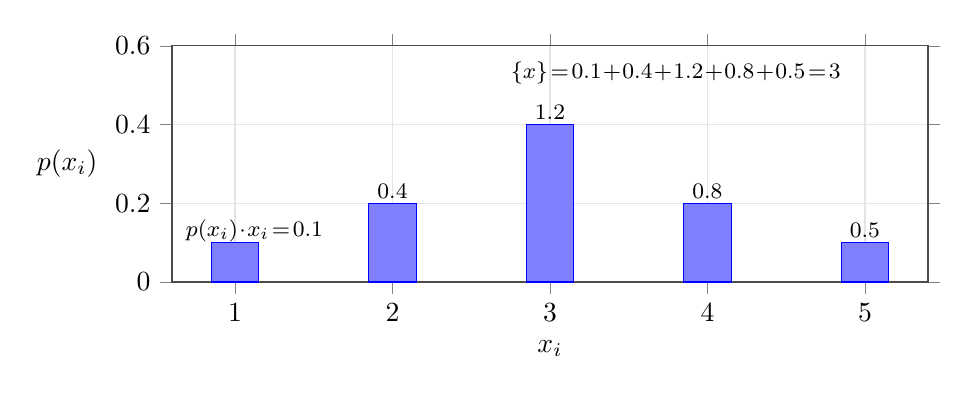
\begin{tikzpicture}
\begin{axis}[
	ybar,
	y=5cm,
	x=2cm,                          % ⬅️ Controls spacing between bars
	bar width=0.6cm,                   % ⬅️ Controls bar thickness
%	bar shift=-0.5cm,                % ⬅️ Center bars (=-0.5 * bar width)
	xlabel={$x_i$},
	clip=false,
	ylabel={$p(x_i)$},
	y label style={rotate=-90, anchor=west, xshift=-1cm},
	xtick={1,2,3,4,5},
	ymin=0, ymax=0.6,
	grid=both,
	major grid style={gray!20},
	tick align=outside,
	axis line style={black!70},
	]
	\addplot+[ybar, fill=blue!50] coordinates {
		(1,0.1) 
		(2,0.2) 
		(3,0.4) 
		(4,0.2)
		(5,0.1)
	};
	% Manual textboxes above bars
	\node[font=\footnotesize,xshift=7pt] at (axis cs:1,0.13) {$p(x_i)\!\cdot\!x_i\!=\!0.1$};
	\node[font=\footnotesize]at (axis cs:2,0.23) {$0.4$};
	\node[font=\footnotesize]at (axis cs:3,0.43) {$1.2$};
	\node[font=\footnotesize] at (axis cs:4,0.23) {$0.8$};
	\node[font=\footnotesize]at (axis cs:5,0.13) {$0.5$};
	\node[font=\footnotesize]at (axis cs:3.8,0.53) {$\expect\{x\}\!=\!0.1\!+\!0.4\!+\!1.2\!+\!0.8\!+\!0.5\!=\!3$};
\end{axis}
\end{tikzpicture}
\end{center}
\vspace*{-5mm}
\caption{The expectation of a discrete \gls{rv} $x$ is obtained by summing up its possible values $x_{i}$, weighted 
	by the corresponding \gls{probability} $p(x_i) = \prob{x= x_i}$. \label{fig_expect_discrete_dict}}
 \end{figure}
		See also: \gls{featurevec}, \gls{realization}, \gls{rv}, \gls{probdist}, \gls{probability}.},
first={expectation},
text={expectation}
}

\newglossaryentry{logreg}
{name={logistic regression}, 
	description={Logistic\index{logistic regression} \gls{regression} learns a 
		linear \gls{hypothesis} \gls{map} (or \gls{classifier}) $\hypothesis(\featurevec) = \weights^{T} \featurevec$ 
		to predict a binary \gls{label} $\truelabel$ based on the numeric \gls{featurevec} $\featurevec$ of 
		a \gls{datapoint}. The quality of a linear \gls{hypothesis} \gls{map} is measured by the average \gls{logloss} 
		on some \glspl{labeled datapoint} (i.e., the \gls{trainset}).
				\\
		See also: \gls{regression}, \gls{hypothesis}, \gls{map}, \gls{classifier}, \gls{label}, \gls{featurevec}, \gls{datapoint}, \gls{logloss}, \gls{labeled datapoint}, \gls{trainset}.},
	first={logistic regression},
	text={logistic regression}
}
	
\newglossaryentry{logloss}
{name={logistic loss}, 
	description={Consider\index{logistic loss} 
		a \gls{datapoint} characterized by the \glspl{feature} $\featurevec$ and a binary \gls{label} $\truelabel \in \{-1,1\}$. 
		We use a real-valued \gls{hypothesis} $\hypothesis$ to predict the \gls{label} $\truelabel$ 
		from the \glspl{feature} $\featurevec$. The logistic \gls{loss} incurred by this \gls{prediction} is 
		defined as 
	\begin{equation} 
		\label{equ_log_loss_gls_dict}
		\lossfunc{(\featurevec,\truelabel)}{\hypothesis} \defeq  \log ( 1 + \exp(- \truelabel \hypothesis(\featurevec))).
	\end{equation}
	\begin{figure}[H]
	\begin{center}
		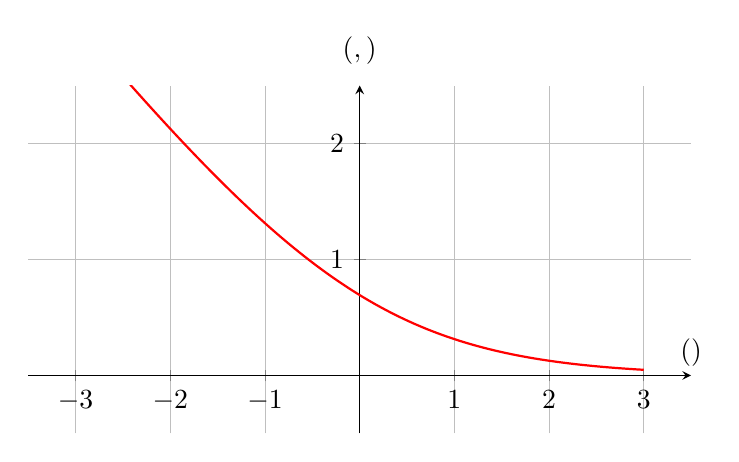
\begin{tikzpicture}
			\begin{axis}[
				axis lines=middle,
				xlabel={$\truelabel\hypothesis(\featurevec)$},
				ylabel={$\lossfunc{(\featurevec,\truelabel)}{\hypothesis}$},
				xlabel style={at={(axis description cs:1.,0.3)}, anchor=north},  % Adjusted to be relative to axis end
				ylabel style={at={(axis description cs:0.5,1.1)}, anchor=center}, % Corrected to vertical position, rotated for readability
				xmin=-3.5, xmax=3.5,
				ymin=-0.5, ymax=2.5,
				xtick={-3, -2, -1, 0, 1, 2, 3},
				ytick={0, 1, 2},
				domain=-3:3,
				samples=100,
				width=10cm, height=6cm,
				grid=both,
				major grid style={line width=.2pt, draw=gray!50},
				minor grid style={line width=.1pt, draw=gray!20},
				legend pos=south west % Positions legend at the bottom left
				]
					\addplot [red, thick] {ln(1 + exp(-x))};    
			\end{axis}
		\end{tikzpicture}
		\caption{The logistic \gls{loss} incurred by the \gls{prediction} $\hypothesis(\featurevec) \in \mathbb{R}$ 
			for a \gls{datapoint} with \gls{label} $\truelabel \in \{-1,1\}$.}
		\label{fig_logloss_dict}
	\end{center}
	\end{figure}
	Carefully note that the expression \eqref{equ_log_loss_gls_dict} 
	for the logistic \gls{loss} applies only for the \gls{labelspace} $\labelspace = \{ -1,1\}$ and when using 
	the thresholding rule \eqref{equ_def_threshold_bin_classifier_dict}. 
		\\
		See also: \gls{datapoint}, \gls{feature}, \gls{label}, \gls{hypothesis}, \gls{loss}, \gls{prediction}, \gls{labelspace}.},
	first={logistic loss},
	text={logistic loss}
}
	
\newglossaryentry{hingeloss}
{name={hinge loss}, 
	description={Consider\index{hinge loss} a \gls{datapoint} 
		characterized by a \gls{featurevec} $\featurevec \in \mathbb{R}^{\featuredim}$ and a 
		binary \gls{label} $\truelabel \in \{-1,1\}$. The hinge \gls{loss} incurred by a real-valued 
		\gls{hypothesis} \gls{map} $\hypothesis(\featurevec)$ is defined as 
		\begin{equation} 
			\label{equ_hinge_loss_gls_dict}
				\lossfunc{(\featurevec,\truelabel)}{\hypothesis} \defeq \max \{ 0 , 1 - \truelabel \hypothesis(\featurevec) \}. 
			\end{equation}
\begin{figure}[H]
\begin{center}
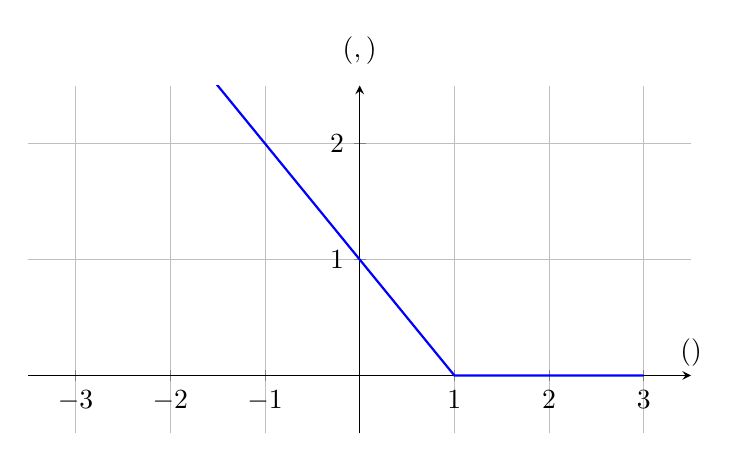
\begin{tikzpicture}
    \begin{axis}[
        axis lines=middle,
        xlabel={$\truelabel\hypothesis(\featurevec)$},
        ylabel={$\lossfunc{(\featurevec,\truelabel)}{\hypothesis}$},
 	xlabel style={at={(axis description cs:1.,0.3)}, anchor=north},  % Adjusted to be relative to axis end
        ylabel style={at={(axis description cs:0.5,1.1)}, anchor=center}, % Corrected to vertical position, rotated for readability
        xmin=-3.5, xmax=3.5,
        ymin=-0.5, ymax=2.5,
        xtick={-3, -2, -1, 0, 1, 2, 3},
        ytick={0, 1, 2},
        domain=-3:3,
        samples=100,
        width=10cm, height=6cm,
        grid=both,
        major grid style={line width=.2pt, draw=gray!50},
        minor grid style={line width=.1pt, draw=gray!20},
        legend pos=south west % Positions legend at the bottom left
    ]
        \addplot[blue, thick] {max(0, 1-x)};
     %   \addlegendentry{$\max(0, 1-x)$}
    \end{axis}
\end{tikzpicture}
\caption{The hinge \gls{loss} incurred by the \gls{prediction} $\hypothesis(\featurevec) \in \mathbb{R}$ 
for a \gls{datapoint} with \gls{label} $\truelabel \in \{-1,1\}$. A regularized variant of the hinge 
\gls{loss} is used by the \gls{svm} \cite{LampertNowKernel}.}
\label{fig_hingeloss_dict}
\end{center}
\end{figure} 	    
		See also: \gls{datapoint}, \gls{featurevec}, \gls{label}, \gls{loss}, \gls{hypothesis}, \gls{map}, \gls{prediction}, \gls{svm}.},
	first={hinge loss},
	text={hinge loss}
}

\newglossaryentry{iidasspt}
{name={independent and identically distributed assumption (i.i.d.\ assumption)}, 
	description={The \gls{iid} assumption\index{independent and identically distributed assumption (i.i.d.\ assumption)} interprets \glspl{datapoint} of a \gls{dataset} as the 
		\glspl{realization} of \gls{iid} \glspl{rv}.
				\\
		See also: \gls{iid}, \gls{datapoint}, \gls{dataset}, \gls{realization}, \gls{rv}.},
	first={independent and identically distributed assumption (i.i.d.\ assumption)},
	text={i.i.d.\ assumption} 
}

\newglossaryentry{hypospace}
{name={hypothesis space}, plural={hypothesis spaces}, 
	description={Every\index{hypothesis space} 
		practical \gls{ml} method uses a \gls{hypothesis} space (or \gls{model}) $\hypospace$. The \gls{hypothesis} space 
		of an \gls{ml} method is a subset of all possible \glspl{map} from the \gls{featurespace} to the \gls{labelspace}. 
		The design choice of the \gls{hypothesis} space should take into account available computational resources and 
		\gls{statasp}. If the computational infrastructure allows for efficient matrix operations, and there 
		is an (approximately) linear relation between a set of \glspl{feature} and a \gls{label}, a useful choice for the 
		\gls{hypothesis} space might be the \gls{linmodel}.
				\\
		See also: \gls{ml}, \gls{hypothesis}, \gls{model}, \gls{map}, \gls{featurespace}, \gls{labelspace}, \gls{statasp}, \gls{feature}, \gls{label}, \gls{linmodel}.},
	first={hypothesis space},
	text={hypothesis space} 
}

	
\newglossaryentry{model}
{name={model}, plural={models}, 
	description={In\index{model} the context of \gls{ml}, 
		the term model typically refers to the \gls{hypospace} underlying an 
		\gls{ml} method \cite{MLBasics}, \cite{ShalevMLBook}. However, the term is also used in other 
		fields but with a different meaning. For example, a \gls{probmodel} refers to a parametrized 
		set of \glspl{probdist}.
				\\
		See also: \gls{ml}, \gls{hypospace}, \gls{probmodel}, \gls{probdist}.},
	first={model},
	text={model} 
}

\newglossaryentry{modelparams}
{name={model parameters}, 
	description={\Gls{model} \glspl{parameter}\index{model parameters} are quantities that 
		are used to select a specific \gls{hypothesis} \gls{map} from a \gls{model}. 
		We can think of a list of \gls{model} \glspl{parameter} as a unique identifier for a \gls{hypothesis} 
		\gls{map}, similar to how a social security number identifies a person in Finland.
			\\
		See also: \gls{model}, \gls{parameter}, \gls{hypothesis}, \gls{map}.},
	first={model parameters},
	text={model parameters} 
}

\newglossaryentry{ai}
{name={artificial intelligence (AI)}, 
	description={AI\index{artificial intelligence (AI)} refers to systems that behave rationally in the sense of 
		maximizing a long-term \gls{reward}. The \gls{ml}-based approach to AI is to train a \gls{model} for  
		predicting optimal actions. These \glspl{prediction} are computed from observations about the state of the 
		environment. The choice of \gls{lossfunc} sets AI applications apart from more basic \gls{ml} applications. 
		AI systems rarely have access to a labeled \gls{trainset} that allows the average \gls{loss} to be measured for any possible choice of \gls{modelparams}. 
		Instead, AI systems use observed \gls{reward} signals to obtain a (point-wise) estimate for the 
		\gls{loss} incurred by the current choice of \gls{modelparams}.
				\\
		See also: \gls{reward}, \gls{ml}, \gls{model}, \gls{lossfunc}, \gls{trainset}, \gls{loss}, \gls{modelparams}.},
	first={AI},
	text={AI} 
}

\newglossaryentry{reward}
{name={reward}, 
	description={A reward refers to some\index{reward} observed 
		(or measured) quantity that allows us to estimate the \gls{loss} incurred by the \gls{prediction} 
		(or decision) of a \gls{hypothesis} $\hypothesis(\featurevec)$. For example, in an 
		\gls{ml} application to self-driving vehicles, $\hypothesis(\featurevec)$ could represent 
		the current steering direction of a vehicle. We could construct a reward from the 
		measurements of a collision sensor that indicate if the vehicle is moving towards 
		an obstacle. We define a low reward for the steering direction 
		$\hypothesis(\featurevec)$ if the vehicle moves dangerously towards an obstacle.
			\\
		See also: \gls{loss}, \gls{prediction}, \gls{hypothesis}, \gls{ml}.},
	first={reward}, 
	text={reward}
} 

\newglossaryentry{hardclustering}
{name={hard clustering}, 
	description={Hard \gls{clustering}\index{hard clustering} 
		refers to the task of partitioning a given set of \glspl{datapoint} into (a few) non-overlapping \glspl{cluster}. 
		The most widely used hard \gls{clustering} method is \gls{kmeans}.
				\\
		See also: \gls{clustering}, \gls{datapoint}, \gls{cluster}, \gls{kmeans}.},
	first={hard clustering},
	text={hard clustering} 
}
	
\newglossaryentry{softclustering}
{name={soft clustering}, 
	description={Soft \gls{clustering}\index{soft clustering} 
		refers to the task of partitioning a given set of \glspl{datapoint} into (a few) overlapping \glspl{cluster}. 
		Each \gls{datapoint} is assigned to several different \glspl{cluster} with varying degrees of belonging. Soft \gls{clustering} 
		methods determine the \gls{dob} (or soft \gls{cluster} assignment) for each \gls{datapoint} and each \gls{cluster}.
		A principled approach to soft \gls{clustering} is by interpreting \glspl{datapoint} as \gls{iid} \glspl{realization} 
		of a \gls{gmm}. We then obtain a natural choice for the \gls{dob} as the conditional 
		\gls{probability} of a \gls{datapoint} belonging to a specific mixture component.
				\\
		See also: \gls{clustering}, \gls{datapoint}, \gls{cluster}, \gls{dob}, \gls{iid}, \gls{realization}, \gls{gmm}, \gls{probability}.},
	first={soft clustering},
	text={soft clustering} 
}


\newglossaryentry{kroneckerproduct}
{name={Kronecker product}, 
	description={The\index{Kronecker product} Kronecker product between two matries $\mA$ and $\mB$ as 
		defined as... 
		},
	first={Kronecker product},
	text={Kronecker product} 
}

	
\newglossaryentry{clustering}
{name={clustering}, 
	description={Clustering\index{clustering} methods decompose a given set 
	 of \glspl{datapoint} into a few subsets, which are referred to as \glspl{cluster}. 
	 Each \gls{cluster} consists of \glspl{datapoint} that are more similar to each 
	 other than to \glspl{datapoint} outside the \gls{cluster}. Different clustering methods 
		use different measures for the similarity between \glspl{datapoint} and different 
		forms of \gls{cluster} representations. The clustering method \gls{kmeans} uses the 
		average \gls{feature} vector of a \gls{cluster} (i.e., the \gls{cluster} \gls{mean}) as its representative. 
		A popular \gls{softclustering} method based on \gls{gmm} represents 
		a \gls{cluster} by a \gls{mvndist}.
				\\
		See also:  \gls{cluster}, \gls{kmeans}, \gls{softclustering}, \gls{gmm}.},
		first={clustering},
		text={clustering} }
	
\newglossaryentry{cluster}
{name={cluster}, 
 plural={clusters}, 
description={A\index{cluster} cluster is a subset of 
		\glspl{datapoint} that are more similar to each other than to the \glspl{datapoint} outside the cluster. 
		The quantitative measure of similarity between \glspl{datapoint} is a design choice. If \glspl{datapoint} 
		are characterized by Euclidean \glspl{featurevec} $\featurevec \in \mathbb{R}^{\nrfeatures}$, 
		we can define the similarity between two \glspl{datapoint} via the Euclidean distance between 
		their \glspl{featurevec}. An example of such clusters is shown in Figure \ref{fig:clusters_dict}.\\
		\begin{figure}[H]
		\centering
		\begin{tikzpicture}
		\pgfplotsset{compat=1.18}
		\begin{axis}[
		    width=10cm,
		    height=8cm,
		    xlabel={$x_1$},
		    ylabel={$x_2$},
		    title={Clusters of Data Points},
		    xmin=0, xmax=10,
		    ymin=0, ymax=10,
		    axis lines=left,
		    legend style={at={(0.5,-0.25)}, anchor=north, legend columns=3}
		]
		% Cluster 1 
		\addplot[only marks, color=blue, mark=*, mark size=3pt] coordinates {
		    (1,1) (2,1.2) (1.8,2) (2.2,1.5) (1.5,2.5)
		};
		% Cluster 2 
		\addplot[only marks, color=red, mark=square*, mark size=3pt] coordinates {
		    (7,8) (8,7.5) (7.5,8.5) (8.2,7.8) (7.7,7)
		};
		% Cluster 3 
		\addplot[only marks, color=green!60!black, mark=triangle*, mark size=3pt] coordinates {
		    (5,3) (5.5,3.2) (5.2,2.8) (4.8,3.5) (5.1,3.1)
		};
		\legend{Cluster 1, Cluster 2, Cluster 3}
		\end{axis}
		\end{tikzpicture}
		\caption{Illustration of three clusters in a two-dimensional \gls{featurespace}. Each cluster groups \glspl{datapoint} that are more similar to each other than to those in other clusters, based on the Euclidean distance.}
		\label{fig:clusters_dict}
		\end{figure}
		See also: \gls{datapoint}, \gls{featurevec}, \gls{featurespace}.
		},
		first={cluster},
		text={cluster} 
		}


\newglossaryentry{huberloss}
{name={Huber loss}, 
	description={The\index{Huber loss} 
		Huber \gls{loss} unifies the \gls{sqerrloss} and the \gls{abserr}.
				\\
		See also: \gls{loss}, \gls{sqerrloss}, \gls{abserr}.},
	first={Huber loss},
	text={Huber loss} 
}


\newglossaryentry{svm}
{name={support vector machine (SVM)}, 
	description={The\index{support vector machine (SVM)} 
		SVM is a binary \gls{classification} method that 
		learns a linear \gls{hypothesis} \gls{map}. Thus, like \gls{linreg} and \gls{logreg}, 
		it is also an instance of \gls{erm} for the \gls{linmodel}. However, the 
		SVM uses a different \gls{lossfunc} from the one used in those methods. As illustrated in 
		Figure \ref{fig_svm_gls_dict}, it aims to maximally separate \glspl{datapoint} from 
		the two different classes in the \gls{featurespace} (i.e., \gls{maximum} margin principle). 
		Maximizing this separation is equivalent to minimizing a regularized 
		variant of the \gls{hingeloss} \eqref{equ_hinge_loss_gls_dict} \cite{BishopBook}, \cite{LampertNowKernel}, \cite{Cristianini_Shawe-Taylor_2000}.
		\begin{figure}[H]
			\begin{center}
				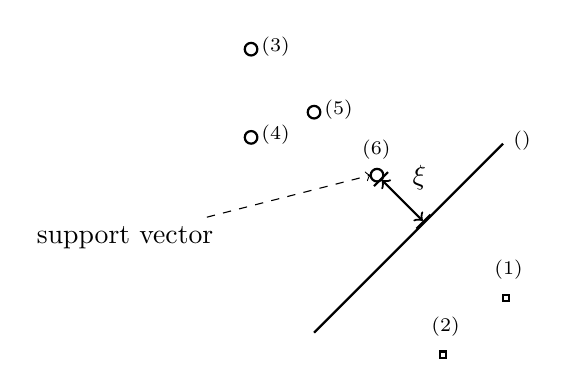
\begin{tikzpicture}[auto,scale=0.8]
					\draw [thick] (1,2) circle (0.1cm)node[anchor=west] {\hspace*{0mm}$\featurevec^{(5)}$};
					\draw [thick] (0,1.6) circle (0.1cm)node[anchor=west] {\hspace*{0mm}$\featurevec^{(4)}$};
					\draw [thick] (0,3) circle (0.1cm)node[anchor=west] {\hspace*{0mm}$\featurevec^{(3)}$};
					\draw [thick] (2,1) circle (0.1cm)node[anchor=east,above] {\hspace*{0mm}$\featurevec^{(6)}$};
					\node[] (B) at (-2,0) {support vector};
					\draw[->,dashed] (B) to (1.9,1) ; 
					\draw [|<->|,thick] (2.05,0.95)  -- (2.75,0.25)node[pos=0.5] {$\xi$} ; 
					\draw [thick] (1,-1.5) -- (4,1.5) node [right] {$\hypothesis^{(\weights)}$} ; 
					\draw [thick] (3,-1.9) rectangle ++(0.1cm,0.1cm) node[anchor=west,above]  {\hspace*{0mm}$\featurevec^{(2)}$};
					\draw [thick] (4,.-1) rectangle ++(0.1cm,0.1cm) node[anchor=west,above] {\hspace*{0mm}$\featurevec^{(1)}$};
				\end{tikzpicture}
				\caption{The SVM learns a \gls{hypothesis} (or \gls{classifier}) $\hypothesis^{(\weights)}$ with 
					minimal average soft-margin \gls{hingeloss}. Minimizing this \gls{loss} is equivalent 
					to maximizing the margin $\xi$ between the \gls{decisionboundary} of $\hypothesis^{(\weights)}$ 
					and each class of the \gls{trainset}.}
				\label{fig_svm_gls_dict}
			\end{center}
		\end{figure}
		The above basic variant of SVM is only useful if the \glspl{datapoint} from different categories can be  
		(approximately) linearly separated. For an \gls{ml} application where the categories are not 
		derived from a \gls{kernel}.
				\\
		See also: \gls{classification}, \gls{hypothesis}, \gls{map}, \gls{linreg}, \gls{logreg}, \gls{erm}, \gls{linmodel}, \gls{lossfunc}, \gls{datapoint}, \gls{featurespace}, \gls{maximum}, \gls{hingeloss}, \gls{svm}, \gls{classifier}, \gls{loss}, \gls{decisionboundary}, \gls{trainset}, \gls{ml}, \gls{kernel}.},
	first={support vector machine (SVM)},
	text={SVM} 
}

\newglossaryentry{eigenvalue}
{name={eigenvalue}, plural={eigenvalues}, 
	description={We\index{eigenvalue} refer to a 
		number $\lambda \in \mathbb{R}$ as an eigenvalue of a square matrix $\mathbf{A} \in \mathbb{R}^{\featuredim \times \featuredim}$ 
		if there is a non-zero vector $\vx \in \mathbb{R}^{\featuredim} \setminus \{ \mathbf{0} \}$ such that $\mathbf{A} \vx = \lambda \vx$.},
	first={eigenvalue},
	text={eigenvalue} 
}
	
\newglossaryentry{eigenvector}
{name={eigenvector}, plural={eigenvectors}, 
	description={An\index{eigenvector} 
		eigenvector of a matrix $\mathbf{A} \in \mathbb{R}^{\featuredim \times \featuredim}$ 
		is a non-zero vector $\vx \in \mathbb{R}^{\featuredim} \setminus \{ \mathbf{0} \}$ 
		such that $\mathbf{A} \vx = \lambda \vx$ with some \gls{eigenvalue} $\lambda$.
				\\
		See also: \gls{eigenvalue}.},
	first={eigenvector},
	text={eigenvector} 
}

\newglossaryentry{evd}
{name={eigenvalue decomposition (EVD)}, 
	description={The\index{eigenvalue decomposition (EVD)} EVD
		for a square matrix $\mA \in \mathbb{R}^{\dimlocalmodel \times \dimlocalmodel}$ 
		is a factorization of the form 
		$$\mA = \mathbf{V} {\bm \Lambda} \mathbf{V}^{-1}.$$ 
		The columns of the matrix $\mV = \big( \vv^{(1)},\ldots,\vv^{(\dimlocalmodel)} \big)$ are the 
		\glspl{eigenvector} of the matrix $\mV$. The diagonal matrix 
		${\bm \Lambda} = {\rm diag} \big\{ \eigval{1},\ldots,\eigval{\dimlocalmodel} \big\}$ 
		contains the \glspl{eigenvalue} $\eigval{\featureidx}$ corresponding to the \glspl{eigenvector} $\vv^{(\featureidx)}$. 
		Note that the above decomposition exists only if the matrix $\mA$ is diagonalizable.
				\\
		See also: \gls{eigenvector}, \gls{eigenvalue}.},
	first={eigenvalue decomposition (EVD)},
	text={EVD} 
}

\newglossaryentry{svd}
{name={singular value decomposition (SVD)}, 
  	description={The\index{singular value decomposition (SVD)} SVD  
  		for a matrix $\mA \in \mathbb{R}^{\samplesize \times \dimlocalmodel}$ 
		is a factorization of the form 
		$$\mA = \mathbf{V} {\bm \Lambda} \mathbf{U}^{T},$$ 
		with orthonormal matrices $\mV \in \mathbb{R}^{\samplesize \times \samplesize}$ 
		and $\mU \in \mathbb{R}^{\dimlocalmodel \times \dimlocalmodel}$ \cite{GolubVanLoanBook}. 
		The matrix ${\bm \Lambda} \in \mathbb{R}^{\samplesize \times \dimlocalmodel}$ is 
		only non-zero along the main diagonal, whose entries $\Lambda_{\featureidx,\featureidx}$ 
		are non-negative and referred to as singular values.},
	first={singular value decomposition (SVD)},
	text={SVD} 
}


\newglossaryentry{tv}
{name={total variation}, 
	description={See \gls{gtv}\index{total variation}.},
	first={total variation},
	text={total variation} 
}


 \newglossaryentry{cvxclustering}
 {name={convex clustering}, 
 	description={Consider\index{convex clustering} a \gls{dataset} 
 		$\featurevec^{(1)},\ldots,\featurevec^{(\samplesize)} \in \mathbb{R}^{\nrfeatures}$. 
 		\Gls{convex} \gls{clustering} learns vectors $\weights^{(1)},\ldots,\weights^{(\samplesize)}$ by minimizing 
 		$$ \sum_{\sampleidx=1}^{\samplesize} \normgeneric{\featurevec^{(\sampleidx)} - \weights^{(\sampleidx)}}{2}^2 + 
 		\regparam \sum_{\nodeidx,\nodeidx' \in \nodes} \normgeneric{\weights^{(\nodeidx)} - \weights^{(\nodeidx')}}{p}.$$ 
		Here, $ \normgeneric{\vu}{p} \defeq \big( \sum_{\featureidx=1}^{\dimlocalmodel} |u_{\featureidx}|^{p} \big)^{1/p}$ 
		denotes the $p$-\gls{norm} (for $p\geq1$).  
		It turns out that many of the optimal vectors $\widehat{\weights}^{(1)},\ldots,\widehat{\weights}^{(\samplesize)}$ 
		coincide. A \gls{cluster} then consists of those \glspl{datapoint} $\sampleidx \in \{1,\ldots,\samplesize\}$ 
		with identical $\widehat{\weights}^{(\sampleidx)}$ \cite{JMLR:v22:18-694}, \cite{Pelckmans2005}. 
			\\
		See also: \gls{dataset}, \gls{convex}, \gls{clustering}, \gls{norm}, \gls{cluster}, \gls{datapoint}. },
 	first={convex clustering},
	text={convex clustering} 
}


\newglossaryentry{gdmethods}
{name={gradient-based methods}, 
	description={\Gls{gradient}-based\index{gradient-based methods} 
		methods are iterative techniques for finding the \gls{minimum} (or \gls{maximum}) 
		of a \gls{differentiable} \gls{objfunc} of the \gls{modelparams}. These 
		methods construct a sequence of approximations to an optimal choice for 
		\gls{modelparams} that results in a \gls{minimum} (or \gls{maximum}) value of the \gls{objfunc}. 
		As their name indicates, \gls{gradient}-based methods use the \glspl{gradient} of the \gls{objfunc} 
		evaluated during previous iterations to construct new, (hopefully) improved \gls{modelparams}. 
		One important example of a \gls{gradient}-based method is \gls{gd}.
				\\
		See also: \gls{gradient}, \gls{minimum}, \gls{maximum}, \gls{differentiable}, \gls{objfunc}, \gls{modelparams}, \gls{gd}.},
	first={gradient-based methods},
	text={gradient-based methods} 
}


\newglossaryentry{sgd}
{name={subgradient descent}, 
	description={\Gls{subgradient}\index{subgradient descent} 
		descent is a \gls{generalization} of \gls{gd} that does not require differentiability of the 
		\gls{function} to be minimized. This \gls{generalization} is obtained by replacing the concept 
		of a \gls{gradient} with that of a \gls{subgradient}. Similar to \glspl{gradient}, also \glspl{subgradient} 
		allow us to construct local approximations of an \gls{objfunc}. The \gls{objfunc} 
		might be the \gls{emprisk} $\emperror\big( \hypothesis^{(\weights)} \big| \dataset \big)$ viewed 
		as a \gls{function} of the \gls{modelparams} $\weights$ that select a \gls{hypothesis} $\hypothesis^{(\weights)} \in \hypospace$.
				\\
		See also: \gls{subgradient}, \gls{generalization}, \gls{gd}, \gls{function}, \gls{gradient}, \gls{objfunc}, \gls{emprisk}, \gls{modelparams}, \gls{hypothesis}.},
	first={subgradient descent},
	text={subgradient descent} 
}
	
\newglossaryentry{stochGD}
{name={stochastic gradient descent (SGD)}, 
	description={SGD\index{stochastic gradient descent (SGD)} 
		is obtained from \gls{gd} by replacing the \gls{gradient} of the \gls{objfunc} 
		with a \gls{stochastic} approximation. A main application of SGD
		is to train a parametrized \gls{model} via \gls{erm} on a \gls{trainset} $\dataset$ that 
		is either very large or not readily available (e.g., when \glspl{datapoint} are stored 
		in a database distributed all over the planet). To evaluate the \gls{gradient} of the 
		\gls{emprisk} (as a \gls{function} of the \gls{modelparams} $\weights$), 
		we need to compute a sum $\sum_{\sampleidx=1}^{\samplesize} \nabla_{\weights} \lossfunc{\datapoint^{(\sampleidx)}}{\weights}$  
		over all \glspl{datapoint} in the \gls{trainset}. We obtain a \gls{stochastic} 
		approximation to the \gls{gradient} by replacing the sum $\sum_{\sampleidx=1}^{\samplesize} \nabla_{\weights} \lossfunc{\datapoint^{(\sampleidx)}}{\weights}$ 
		with a sum $\sum_{\sampleidx \in \batch} \nabla_{\weights} \lossfunc{\datapoint^{(\sampleidx)}}{\weights}$ 
		over a randomly chosen subset $\batch \subseteq \{1,\ldots,\samplesize\}$ (see Figure \ref{fig_sgd_approx_dict}). 
		We often refer to these randomly chosen \glspl{datapoint} as a \gls{batch}. 
		The \gls{batch} size $|\batch|$ is an important \gls{parameter} of SGD. 
		SGD with $|\batch|> 1$ is referred to as mini-\gls{batch} SGD \cite{Bottou99}. 		
		\begin{figure}[H]
			\centering
			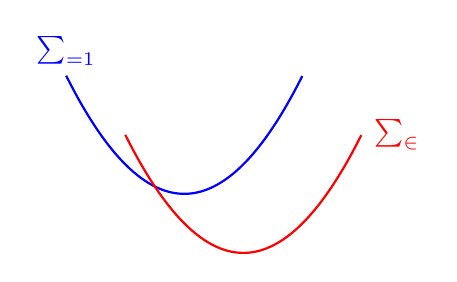
\begin{tikzpicture}[scale=1.5, >=stealth]
				\draw[thick, blue, domain=0.5:2.5, samples=100] plot (\x, {(\x-1.5)^2 + 1});
				\node[blue,above] at (0.5, 2) {$\sum_{\sampleidx=1}^{\samplesize}$};
				\draw[thick, red, domain=1:3, samples=100] plot (\x, {(\x-2)^2 + 0.5});
				\node[red] at (3.3, 1.5) {$\sum_{\sampleidx \in \batch}$};
			\end{tikzpicture}
		\caption{SGD for \gls{erm} approximates the \gls{gradient} 
		$\sum_{\sampleidx=1}^{\samplesize} \nabla_{\weights} \lossfunc{\datapoint^{(\sampleidx)}}{\weights}$ 
		by replacing the 
		sum over all \glspl{datapoint} in the \gls{trainset} (indexed by $\sampleidx=1,\ldots,\samplesize$) 
		with a sum over a randomly chosen subset $\batch \subseteq \{1,\ldots,\samplesize\}$.\label{fig_sgd_approx_dict}}
		\end{figure}
		See also: \gls{gd}, \gls{gradient}, \gls{objfunc}, \gls{stochastic}, \gls{model}, \gls{erm}, \gls{trainset}, \gls{datapoint}, \gls{emprisk}, \gls{function}, \gls{modelparams}, \gls{batch}, \gls{parameter}.},
	first={stochastic gradient descent (SGD)},
	text={SGD} 
}


\newglossaryentry{onlineGD}
{name={online gradient descent (online GD)}, 
	description={Consider \index{online gradient descent (online GD)} an \gls{ml} method that learns \gls{modelparams} 
		$\weights$ from some \gls{paramspace} $\paramspace \subseteq \mathbb{R}^{\dimlocalmodel}$. 
		The learning process uses \glspl{datapoint} $\datapoint^{(\timeidx)}$ that arrive at consecutive time-instants $\timeidx=1,2,\ldots$. 
		Let us interpret the \glspl{datapoint} $\datapoint^{(\timeidx)}$ as \gls{iid} copies 
		of an \gls{rv} $\datapoint$. The \gls{risk} $\expect\{ \lossfunc{\datapoint}{\weights} \}$ of a 
		\gls{hypothesis} $\hypothesis^{(\weights)}$ can then (under mild conditions) be obtained as the limit 
		$\lim_{T\rightarrow \infty} (1/T)\sum_{\timeidx=1}^{T} \lossfunc{\datapoint^{(\timeidx)}}{\weights}$. 
		We might use this limit as the \gls{objfunc} for learning the \gls{modelparams} $\weights$. 
		Unfortunately, this limit can only be evaluated if we wait infinitely long in order to collect all \glspl{datapoint}. 
		Some \gls{ml} applications require methods that learn online, i.e., as soon as a new \gls{datapoint} $\datapoint^{(\timeidx)}$ 
		arrives at time $\timeidx$, we update the current \gls{modelparams} $\weights^{(\timeidx)}$. Note that 
		the new \gls{datapoint} $\datapoint^{(\timeidx)}$ contributes the component $\lossfunc{\datapoint^{(\timeidx)}}{\weights}$ 
		to the \gls{risk}. As its name suggests, online \gls{gd} updates $\weights^{(\timeidx)}$ via a (projected) \gls{gradstep} such that
		\begin{equation} 
			\label{equ_def_ogd_dict}
 			\weights^{(\timeidx+1)} \defeq \projection{\paramspace}{\weights^{(\timeidx)} - \lrate_{\timeidx} \nabla_{\weights} \lossfunc{\datapoint^{(\timeidx)}}{\weights}}. 
		\end{equation} 
		Note that \eqref{equ_def_ogd_dict} is a \gls{gradstep} for the current component $\lossfunc{\datapoint^{(\timeidx)}}{\cdot}$ 
		of the \gls{risk}. The update \eqref{equ_def_ogd_dict} ignores all the previous components $\lossfunc{\datapoint^{(\timeidx')}}{\cdot}$, 
		for $\timeidx' < \timeidx$. It might therefore happen that, compared to $\weights^{(\timeidx)}$, the updated \gls{modelparams} 
		$\weights^{(\timeidx+1)}$ increase the retrospective average \gls{loss} $\sum_{\timeidx'=1}^{\timeidx-1} \lossfunc{\datapoint^{(\timeidx')}}{\cdot}$. 
		However, for a suitably chosen \gls{learnrate} $\lrate_{\timeidx}$, online \gls{gd} can be shown 
		to be optimal in practically relevant settings. By optimal, we mean that the \gls{modelparams} 
		$\weights^{(T+1)}$ delivered by online \gls{gd} after observing $T$ \glspl{datapoint} $\datapoint^{(1)},\ldots, \datapoint^{(T)}$ 
		are at least as good as those delivered by any other learning method \cite{HazanOCO}, \cite{GDOptimalRakhlin2012}. 
\begin{figure}[H]
	\begin{center}
\begin{tikzpicture}[x=1.5cm,scale=1.5, every node/.style={font=\footnotesize}]
	\draw[->] (0.5, 0) -- (5.5, 0) node[below] {};
	\foreach \x in {1, 2, 3, 4, 5} {
		\draw (\x, 0.1) -- (\x, -0.1) node[below] {$t=\x$};
	}
	\foreach \x/\y in {1/2.5, 2/1.8, 3/2.3, 4/1.5, 5/2.0} {
		\fill[black] (\x, \y) circle (2pt) node[above right] {$\datapoint^{(\x)}$};
	}
	\foreach \x/\y in {1/1.0, 2/1.6, 3/1.8, 4/2.2, 5/1.9} {
		\fill[blue] (\x, \y) circle (2pt) node[below left] {$\weights^{(\x)}$};
	}
	\foreach \x/\y/\z in {1/2.5/1.0, 2/1.8/1.6, 3/2.3/2.0, 4/1.5/1.8, 5/2.0/1.9} {
		\draw[dashed, gray] (\x, \y) -- (\x, \z);
	}
	\end{tikzpicture}
\end{center} 
\caption{An instance of online \gls{gd} that updates the \gls{modelparams} $\weights^{(\timeidx)}$ 
using the \gls{datapoint} $\datapoint^{(\timeidx)} = \feature^{(\timeidx)}$ arriving at time $\timeidx$. 
This instance uses the \gls{sqerrloss} $\lossfunc{\datapoint^{(\timeidx)}}{\weight} = (\feature^{(\timeidx)} - \weight)^{2}$.}
\end{figure}
		See also: \gls{ml}, \gls{modelparams}, \gls{paramspace}, \gls{datapoint}, \gls{iid}, \gls{rv}, \gls{risk}, \gls{hypothesis}, \gls{objfunc}, \gls{gd}, \gls{gradstep}, \gls{loss}, \gls{learnrate}, \gls{sqerrloss}.},
	first={online gradient descent (online GD)},
	text={online GD}
}

\newglossaryentry{pca}
{name={principal component analysis (PCA)}, 
	description={PCA\index{principal component analysis (PCA)} 
		determines a linear \gls{featuremap} such that the new \glspl{feature} 
		allow us to reconstruct the original \glspl{feature} with the \gls{minimum} reconstruction error \cite{MLBasics}.
				\\
		See also: \gls{featuremap}, \gls{feature}, \gls{minimum}.},
	first={principal component analysis (PCA)},
	text={PCA} 
}
	
\newglossaryentry{loss}
{name={loss}, 
	description={\gls{ml}\index{loss} methods use a 
		\gls{lossfunc} $\lossfunc{\datapoint}{\hypothesis}$ to measure the error incurred 
		by applying a specific \gls{hypothesis} to a specific \gls{datapoint}. With a
		slight abuse of notation, we use the term loss for both the \gls{lossfunc} $\loss$ 
		itself and the specific value $\lossfunc{\datapoint}{\hypothesis}$, for a \gls{datapoint} $\datapoint$ 
		and \gls{hypothesis} $\hypothesis$.
				\\
		See also: \gls{ml}, \gls{lossfunc}, \gls{hypothesis}, \gls{datapoint}.},
	first={loss},
	text={loss} 
}

\newglossaryentry{lossfunc}
{name={loss function}, 
	description={A\index{loss function} \gls{loss} \gls{function} is a \gls{map} 
		$$\lossfun: \featurespace \times \labelspace \times \hypospace \rightarrow \mathbb{R}_{+}: \big( \big(\featurevec,\truelabel\big),
		 \hypothesis\big) \mapsto  \lossfunc{(\featurevec,\truelabel)}{\hypothesis}.$$
		It assigns a non-negative real number (i.e., the \gls{loss}) $\lossfunc{(\featurevec,\truelabel)}{\hypothesis}$
		to a pair that consists of a \gls{datapoint}, with \glspl{feature} $\featurevec$ 
		and \gls{label} $\truelabel$, and a \gls{hypothesis} $\hypothesis \in \hypospace$. The 
		value $\lossfunc{(\featurevec,\truelabel)}{\hypothesis}$ quantifies the discrepancy 
		between the true \gls{label} $\truelabel$ and the \gls{prediction} $\hypothesis(\featurevec)$. 
		Lower (closer to zero) values $\lossfunc{(\featurevec,\truelabel)}{\hypothesis}$ indicate a smaller 
		discrepancy between \gls{prediction} $\hypothesis(\featurevec)$ and \gls{label} $\truelabel$. 
		Figure \ref{fig_loss_function_gls_dict} depicts a \gls{loss} \gls{function} for a given \gls{datapoint}, 
		with \glspl{feature} $\featurevec$ and \gls{label} $\truelabel$, as a \gls{function} of the \gls{hypothesis} $\hypothesis \in \hypospace$. 
		\begin{figure}[H]
			\begin{center}
				\begin{tikzpicture}[scale = 0.7]
					\begin{axis}
						[axis x line=center,
						axis y line=center,
						xlabel={},
						xlabel style={below right},
						ylabel style={above right},
						xtick=\empty,
						ytick=\empty,
						xmin=-4,
						xscale = 1.4, 
						xmax=4,
						ymin=-0.5,
						ymax=2.5
						]
						\addplot [red, thick] {ln(1 + exp(-x))};    
					\end{axis}
					\node [above,centered,xshift=-5pt] at (1,5) {$\lossfunc{(\featurevec,\truelabel)}{\hypothesis}$};
					\node [above] at (10,1) {\gls{hypothesis} $\hypothesis$};
						\node [right] at (4,6) {\gls{loss}};
				\end{tikzpicture}
			\end{center}
			\vspace*{-7mm}
			\caption{Some \gls{loss} \gls{function} $\lossfunc{(\featurevec,\truelabel)}{\hypothesis}$ for a fixed \gls{datapoint}, with 
				\gls{featurevec} $\featurevec$ and \gls{label} $\truelabel$, and a varying \gls{hypothesis} $\hypothesis$. 
				\gls{ml} methods try to find (or learn) a \gls{hypothesis} that incurs minimal \gls{loss}.}
			\label{fig_loss_function_gls_dict}
		\end{figure}
		See also: \gls{loss}, \gls{function}, \gls{map}, \gls{datapoint}, \gls{feature}, \gls{label}, \gls{hypothesis}, \gls{prediction}, \gls{featurevec}, \gls{ml}.},
 	first={loss function},
 	text={loss function} 
}

\newglossaryentry{decisiontree}
{name={decision tree}, plural={decision trees}, 
	description={A\index{decision tree} 
		decision tree is a flow-chart-like representation of a \gls{hypothesis} \gls{map} $\hypothesis$. 
		More formally, a decision tree is a directed \gls{graph} containing a root node that reads 
		in the \gls{featurevec} $\featurevec$ of a \gls{datapoint}. The root node then forwards 
		the \gls{datapoint} to one of its child nodes based on some elementary test on the \glspl{feature} $\featurevec$. 
		If the receiving child node is not a leaf node, i.e., it has itself child nodes, 
	  	it represents another test. Based on the test result, the \gls{datapoint} is forwarded 
	   	to one of its descendants. This testing and forwarding of the \gls{datapoint} is continued 
	  	until the \gls{datapoint} ends up in a leaf node without any children. 
\begin{figure}[H]
\begin{minipage}{.45\textwidth}
	\scalebox{1}{
\begin{tikzpicture}
	\node[fill=black, circle, inner sep=2pt, label=above:{$\| \featurevec-\mathbf{u} \| \leq \varepsilon$?}] (A) {};	
	\node[fill=black, circle, inner sep=2pt, below left=1.5cm and 1cm of A, label=left:{$\hypothesis(\featurevec) = \predictedlabel_1$}] (B) {};
	\node[fill=black, circle, inner sep=2pt, below right=1.5cm and 1cm of A, label=right:{$\| \featurevec - \mathbf{v} \| \leq \varepsilon$?}] (C) {};
	\node[fill=black, circle, inner sep=2pt, below left=1.5cm and 1cm of C, label=left:{$\hypothesis(\featurevec) = \predictedlabel_2$}] (D) {};
	\node[fill=black, circle, inner sep=2pt, below right=1.5cm and 1cm of C, label=right:{$\hypothesis(\featurevec) =\predictedlabel_3$}] (E) {};
	\draw[line width=1.5pt, ->] (A) -- (B) node[midway, left] {no};
	\draw[line width=1.5pt, ->] (A) -- (C) node[midway, right] {yes};
	\draw[line width=1.5pt, ->] (C) -- (D) node[midway, left] {no};
	\draw[line width=1.5pt, ->] (C) -- (E) node[midway, right] {yes};
\end{tikzpicture}
	}
\end{minipage}	
\hspace*{15mm}
\begin{minipage}{.45\textwidth}
	\hspace*{15mm}
	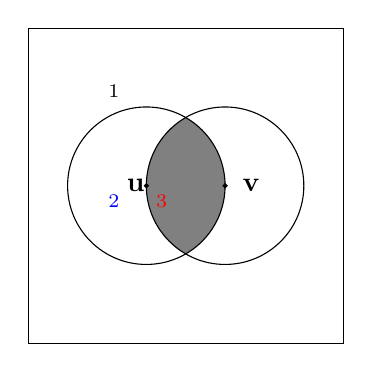
\begin{tikzpicture}
		\draw (-2,2) rectangle (2,-2);
		\begin{scope}
			\clip (-0.5,0) circle (1cm);
			\clip (0.5,0) circle (1cm);
			\fill[color=gray] (-2,1.5) rectangle (2,-1.5);
		\end{scope}
		\draw (-0.5,0) circle (1cm);
		\draw (0.5,0) circle (1cm);
		\draw[fill] (-0.5,0) circle [radius=0.025];
		\node [below right, red] at (-0.5,0) {$\predictedlabel_{3}$};
		\node [below left, blue] at (-0.7,0) {$\predictedlabel_{2}$};
		\node [above left] at (-0.7,1) {$\predictedlabel_{1}$};
		\node [left] at (-0.4,0) {$\mathbf{u}$};
		\draw[fill] (0.5,0) circle [radius=0.025];
		\node [right] at (0.6,0) {$\mathbf{v}$};
	\end{tikzpicture}
\end{minipage}
	\caption{Left: A decision tree is a flow-chart-like representation of a piece-wise 
	    constant \gls{hypothesis} $\hypothesis: \featurespace \rightarrow \mathbb{R}$.  Each piece is a \gls{decisionregion} $\decreg{\predictedlabel} \defeq \big\{ \featurevec \in  \featurespace: \hypothesis(\featurevec) = \predictedlabel \big\}$. 
		The depicted decision tree can be applied to numeric \glspl{featurevec}, i.e., $\featurespace \subseteq \mathbb{R}^{\dimlocalmodel}$. It is  parametrized by the threshold $\varepsilon>0$ and the vectors $\vu, \vv \in \mathbb{R}^{\dimlocalmodel}$. 
		Right: A decision tree partitions  
		the \gls{featurespace} $\featurespace$ into \glspl{decisionregion}. Each \gls{decisionregion}  
		$\decreg{\hat{\truelabel}} \!\subseteq\!\featurespace$ corresponds to a specific leaf node in the decision tree.}
	\label{fig_decision_tree_dict}
\end{figure} 
		See also: \gls{decisionregion}.
	  },first={decision tree},
      text={decision tree} }



\newglossaryentry{API} 
{name={application programming interface (API)},
		description={An \index{application programming interface (API)} API is a formal mechanism that 
			allows software components to interact in a structured and modular way \cite{RestfulBook2013}.
			In the context of \gls{ml}, APIs are commonly used to provide access to a trained \gls{ml} \gls{model}. 
			Users—whether humans or machines—can submit the \gls{featurevec} of a \gls{datapoint} and receive 
			a corresponding \gls{prediction}. Suppose a trained \gls{ml} \gls{model} is defined 
			as $\widehat{\hypothesis}(\feature) \defeq 2 \feature + 1$. Through an API, a user 
			can input $\feature = 3$ and receive the output $\widehat{\hypothesis}(3) = 7$ 
			without knowledge of the detailed structure of the \gls{ml} \gls{model} or its training. 
			In practice, the \gls{model} is typically deployed on a server connected to the internet. 
			Clients send requests containing \gls{feature} values to the server, which responds with 
			the computed \gls{prediction} $\widehat{\hypothesis}(\featurevec)$. APIs promote modularity 
			in \gls{ml} system design, i.e., one team can develop and train the \gls{model}, while another team
			handles integration and user interaction. Publishing a trained \gls{model} via an API also 
			offers practical advantages: 
			\begin{itemize} 
				\item The server can centralize computational resources which are required to compute \glspl{prediction}. 
		        \item The internal structure of the \gls{model} remains hidden—which is useful for protecting intellectual property or trade secrets. 
		    	\end{itemize} 
			However, APIs are not without \gls{risk}. Techniques such as \gls{modelinversion} can potentially reconstruct a 
			\gls{model} from its \glspl{prediction} on carefully selected \glspl{featurevec}.
					\\
			See also: \gls{ml}, \gls{model}, \gls{featurevec}, \gls{datapoint}, \gls{prediction}, \gls{feature}, \gls{modelinversion}.},
		first={application programming interface (API)},
		text={API}
}

\newglossaryentry{modelinversion}
{name={model inversion},
  description={A\index{model inversion} \gls{model} inversion is a form of \gls{privattack} on an \gls{ml} system. 
  	An adversary seeks to infer \glspl{sensattr} of individual \glspl{datapoint} by exploiting partial access 
  	to a trained \gls{model} $\learnthypothesis \in \hypospace$. This access typically consists of 
  	querying the \gls{model} for \glspl{prediction} $\learnthypothesis(\featurevec)$ on carefully chosen inputs. 
  	Basic \gls{model} inversion techniques have been demonstrated in the context of facial image 
  	\gls{classification}, where images are reconstructed using the (\gls{gradient} of) \gls{model} outputs 
  	combined with auxiliary information such as a person’s name \cite{Fredrikson2015}.
  	\begin{figure}[H]
	\begin{center}
	\begin{tikzpicture}[scale=1.5]
  		% Axes
  		\draw[->] (-0.5,0) -- (5.5,0) node[right] {face image $\featurevec$};
  		\draw[->] (0,-0.2) -- (0,2.5) node[above] {name};
  		% Sigmoid-like curve
  		\draw[thick, domain=0.5:5, samples=100, smooth, variable=\x, name path=sigmoid] 
  		plot ({\x}, {2/(1 + exp(-3*(\x - 3)))});
  		%\node at (5.1, 0.2) {\small (e.g., face photo)};
  		% Highlight point
  		\def\xval{3}
  		\pgfmathsetmacro{\yval}{2/(1 + exp(-3*(\xval - 3)))}
  		% Ruler lines
  		\draw[dashed] (\xval,0) -- (\xval,\yval);
  		\draw[dashed] (0,\yval) -- (\xval,\yval);
  		% Filled circle
  		\filldraw[fill=blue!20, draw=blue] (\xval,\yval) circle (0.1);
  		\node[anchor=south east] at (-0.1,\yval) {\footnotesize ``Alexander Jung''};
  		% Axis labels with image
  		\node[anchor=north] at (\xval,-0.25) {\includegraphics[width=1cm]{assets/AlexanderJung.jpg}}; % Replace 'face.jpg' with your image
  		% Label on curve
  		\node[above right] at (4,2.2) {trained \gls{model} $\learnthypothesis$};
  	\end{tikzpicture}
	\end{center} 
	\end{figure}
  	See also: \gls{model}, \gls{privattack}, \gls{ml}, \gls{sensattr}, \gls{datapoint}, \gls{prediction}, \gls{classification}, \gls{gradient}, \gls{trustAI}, \gls{privprot}. },
  first={model inversion},
  text={model inversion}
}


\newglossaryentry{hilbertspace}
{name={Hilbert space},
	description={A\index{Hilbert space} Hilbert space is a complete inner 
		product space \cite{introhilbertbook}. That is, it is a \gls{vectorspace} equipped 
		with an inner product between pairs of vectors, and it satisfies the additional requirement 
		of completeness, i.e., every Cauchy sequence of vectors converges to a limit within the space. 
		A canonical example of a Hilbert space is the \gls{euclidspace} $\mathbb{R}^{\featuredim}$, 
		for some dimension $\featuredim$, consisting of vectors $\vu = \big(u_1, \ldots, u_{\featuredim}\big)^T$ 
		and the standard inner product $\vu^T \vv$.
				\\
		See also: \gls{vectorspace}, \gls{euclidspace}.},
	first={Hilbert space},
	text={Hilbert space}
}



\newglossaryentry{sample}
{name={sample}, plural={samples}, 
	description={A\index{sample} 
		finite sequence (or list) of \glspl{datapoint} $\datapoint^{(1)},\ldots,\datapoint^{(m)}$ that 
		is obtained or interpreted as the \gls{realization} of $\samplesize$ \gls{iid} \glspl{rv} 
		with a common \gls{probdist} $p(\datapoint)$. The length $\samplesize$ of 
		the sequence is referred to as the \gls{samplesize}.
				\\
		See also: \gls{datapoint}, \gls{realization}, \gls{iid}, \gls{rv}, \gls{probdist}, \gls{samplesize}.},
		first={sample},
		text={sample}
}
	
\newglossaryentry{samplesize}
{name={sample size},
	description={The\index{sample size} number of individual \glspl{datapoint} 
		contained in a \gls{dataset}.
				\\
		See also: \gls{datapoint}, \gls{dataset}.},
	first={sample size},
	text={sample size}
}

\newglossaryentry{ann}
{name={artificial neural network (ANN)}, plural={ANNs},
	description={An\index{artificial neural network (ANN)} ANN 
		is a graphical (signal-flow) representation of a \gls{function} that maps 
		\glspl{feature} of a \gls{datapoint} at its input to a \gls{prediction} 
		for the corresponding \gls{label} at its output. The fundamental unit of an 
		ANN is the artificial neuron, which applies an \gls{actfun} to its 
		weighted inputs. The outputs of these neurons serve as inputs for other neurons, 
		forming interconnected layers.
				\\
		See also: \gls{function}, \gls{feature}, \gls{datapoint}, \gls{prediction}, \gls{label}, \gls{actfun}.},
	first={artificial neural network (ANN)},
	text={ANN}
}


\newglossaryentry{randomforest}
{name={random forest},
	description={A\index{random forest} random forest is a set of different \glspl{decisiontree}. 
		Each of these \glspl{decisiontree} is obtained by fitting a perturbed copy of 
		the original \gls{dataset}.
				\\
	See also: \gls{decisiontree}, \gls{dataset}.},
	first={random forest}, 
	text={random forest}
}

\newglossaryentry{bagging}
{name={bagging (or bootstrap aggregation)},
	description={Bagging\index{bagging (or bootstrap aggregation)} (or bootstrap aggregation) 
		is a generic technique to improve (the \gls{robustness} of) a given \gls{ml} method. 
		The idea is to use the \gls{bootstrap} to generate perturbed copies of a given \gls{dataset} 
		and then to learn a separate \gls{hypothesis} for each copy. We then predict the 
		\gls{label} of a \gls{datapoint} by combining or aggregating the individual \glspl{prediction} 
		of each separate \gls{hypothesis}. For \gls{hypothesis} \glspl{map} delivering numeric \gls{label} 
		values, this aggregation could be implemented by computing the average of individual 
		\glspl{prediction}.
				\\
		See also: \gls{robustness}, \gls{ml}, \gls{bootstrap}, \gls{dataset}, \gls{hypothesis}, \gls{label}, \gls{datapoint}, \gls{prediction}, \gls{map}.},
	first={bagging (or bootstrap aggregation)},
	text={bagging}
}


\newglossaryentry{gd}
{name={gradient descent (GD)},
	description={GD\index{gradient descent (GD)} 
		is an iterative method for finding the \gls{minimum} of a \gls{differentiable} 
		\gls{function} $f(\weights)$ of a vector-valued argument $\weights \in \mathbb{R}^{\featurelen}$. 
		Consider a current guess or approximation $\weights^{(\itercntr)}$ for the \gls{minimum} of 
		the \gls{function} $f(\weights)$. We would like to find a new (better) vector $\weights^{(\itercntr+1)}$ 
		that has a smaller objective value $f(\weights^{(\itercntr+1)}) < f\big(\weights^{(\itercntr)}\big)$ than 
		the current guess $\weights^{(\itercntr)}$. We can achieve this typically by using a \gls{gradstep}
		\begin{equation} 
			\label{equ_def_GD_step_dict}
			\weights^{(\itercntr\!+\!1)} = \weights^{(\itercntr)} - \lrate \nabla f(\weights^{(\itercntr)})
		\end{equation} 
		with a sufficiently small \gls{stepsize} $\lrate\!>\!0$. Figure \ref{fig_basic_GD_step_dict} illustrates the effect of 
		a single GD step \eqref{equ_def_GD_step_dict}.
		\begin{figure}[H]
			\begin{center}
				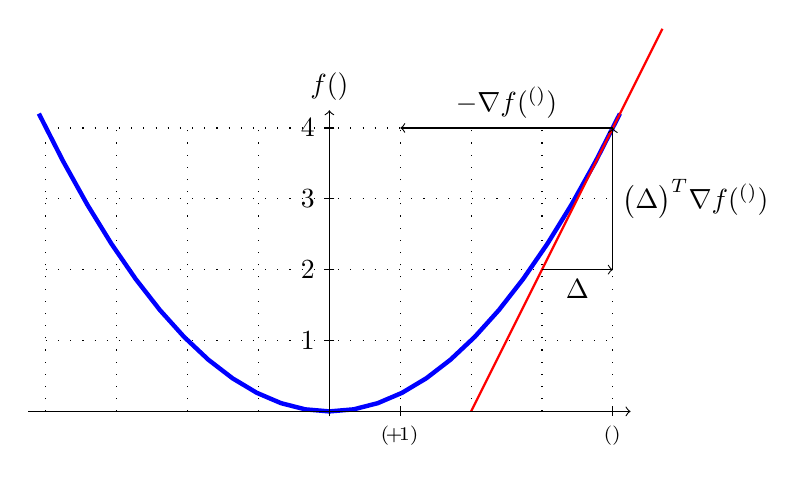
\begin{tikzpicture}[scale=0.9]
					\draw[loosely dotted] (-4,0) grid (4,4);
					\draw[blue, ultra thick, domain=-4.1:4.1] plot (\x,  {(1/4)*\x*\x});
					\draw[red, thick, domain=2:4.7] plot (\x,  {2*\x - 4});
					\draw[<-] (4,4) -- node[right] {$\big( \Delta \weights\big)^{T} \nabla f(\weights^{(\itercntr)})$} (4,2);
					\draw[->] (4,4) -- node[above] {$-\lrate \nabla f(\weights^{(\itercntr)})$} (1,4);
					\draw[<-] (4,2) -- node[below] {$\Delta \weights$} (3,2) ;
					\draw[->] (-4.25,0) -- (4.25,0) node[right] {$\weights$};
					\draw[->] (0,-2pt) -- (0,4.25) node[above] {$f(\weights)$};
					\draw[shift={(0,0)}] (0pt,2pt) -- (0pt,-2pt) node[below] {$\overline{\weights}$};
					\draw[shift={(4,0)}] (0pt,2pt) -- (0pt,-2pt) node[below] {$\weights^{(\itercntr)}$};
					\draw[shift={(1,0)}] (0pt,2pt) -- (0pt,-2pt) node[below] {$\weights^{(\itercntr\!+\!1)}$};
					\foreach \y/\ytext in {1/1, 2/2, 3/3, 4/4}
					\draw[shift={(0,\y)}] (2pt,0pt) -- (-2pt,0pt) node[left] {$\ytext$};  
				\end{tikzpicture}
			\end{center}
			\caption{A single \gls{gradstep} \eqref{equ_def_GD_step_dict} towards the minimizer $\overline{\weights}$ of $f(\weights)$.}
			\label{fig_basic_GD_step_dict}
		\end{figure}
		See also: \gls{minimum}, \gls{differentiable}, \gls{gradstep}, \gls{stepsize}, \gls{gradient}.	
		},
		first={gradient descent (GD)},
		text={GD}
	}

\newglossaryentry{abserr}
{name={absolute error loss},
	description={Consider a \gls{datapoint} with \glspl{feature} $\featurevec \in \featurespace$ and numeric 
		\gls{label} $\truelabel \in \mathbb{R}$. The absolute error \gls{loss}\index{absolute error loss} 
		incurred by a \gls{hypothesis} $\hypothesis: \featurespace \rightarrow \mathbb{R}$ 
		is defined as $|\truelabel - \hypothesis(\featurevec)|$, i.e., the absolute difference between 
		the \gls{prediction} $\hypothesis(\featurevec)$ and the true \gls{label} $\truelabel$.
					\\
		See also: \gls{datapoint}, \gls{feature}, \gls{label}, \gls{loss}, \gls{hypothesis}, \gls{prediction}.},
	first={absolute error loss},
	text={absolute error loss}
}

\newglossaryentry{device}
{name={device}, plural={devices}, 
	description={Any\index{device} physical system that can be used to store and process \gls{data}. In the context of \gls{ml}, 
		we typically mean a computer that is able to read in \glspl{datapoint} from different 
		sources and, in turn, to train an \gls{ml} \gls{model} using these \glspl{datapoint}.
						\\
		See also: \gls{data}, \gls{ml}, \gls{datapoint}, \gls{model}.},
	first={device},
	text={device}
}

\newglossaryentry{llm}
{name={large language model (LLM)},
	description={LLMs\index{large language model (LLM)} is an umbrella term for \gls{ml} methods 
		that process and generate human-like text. These methods typically 
		use \glspl{deepnet} with billions (or even trillions) of \glspl{parameter}. 
		A widely used choice for the network architecture is referred to as 
		Transformers \cite{vaswani2017attention}. The training of LLMs is often  
		based on the task of predicting a few words that are intentionally removed 
		from a large text corpus. Thus, we can construct \glspl{labeled datapoint} 
		simply by selecting some words of a text as \glspl{label} and the remaining 
		words as \glspl{feature} of \glspl{datapoint}. This construction requires 
		very little human supervision and allows for generating sufficiently 
		large \glspl{trainset} for LLMs.
			\\
		See also: \gls{deepnet}, \gls{labeled datapoint}.},
		first={large language model (LLM)},
		text={LLM}
}


\newglossaryentry{huberreg}
{name={Huber regression},
 description={Huber \gls{regression}\index{Huber regression} refers to \gls{erm}-based methods 
			that use the \gls{huberloss} as a measure of the \gls{prediction} error. Two important special cases 
			of Huber \gls{regression} are \gls{ladregression} and \gls{linreg}. Tuning the threshold \gls{parameter} 
			of the \gls{huberloss} allows the user to trade the \gls{robustness} of the \gls{abserr} against 
			the computational benefits of the \gls{smooth} \gls{sqerrloss}.
					\\
		See also: \gls{ladregression}, \gls{linreg}, \gls{abserr}, \gls{sqerrloss}.},
			first={Huber regression},text={Huber regression}}


\newglossaryentry{ladregression}
{name={least absolute deviation regression},
 description={Least\index{least absolute deviation regression} absolute deviation regression 
 	is an instance of \gls{erm} using the \gls{abserr}. It is a special case of \gls{huberreg}.
				\\
 See also: \gls{erm}, \gls{abserr}, \gls{huberreg}.},
 first={least absolute deviation regression},
 text={least absolute deviation regression}
}

\newglossaryentry{metric}
{name={metric},
  description={In its most general form, a\index{metric} metric is a quantitative measure 
  		used to compare or evaluate objects. In mathematics, a metric measures the distance 
		between two points and must follow specific rules, i.e., the distance is always non-negative, 
		zero only if the points are the same, symmetric, and it satisfies the triangle inequality \cite{RudinBookPrinciplesMatheAnalysis}. 
		In \gls{ml}, a metric is a quantitative measure of how well a \gls{model} performs. Examples include \gls{acc}, 
		precision, and the average \gls{zerooneloss} on a \gls{testset} \cite{Goodfellow-et-al-2016}, \cite{BishopBook}. 
		A \gls{lossfunc} is used to train \glspl{model}, while a metric is used to compare trained \glspl{model}.
		\\ See also: \gls{ml}, \gls{model}, \gls{acc}, \gls{zerooneloss}, \gls{testset}, \gls{lossfunc}, \gls{loss}, \gls{modelsel}.},
	first={metric}, 
  text={metric}
 }

\newglossaryentry{bayesrisk}
{name={Bayes risk},
 description={Consider a \gls{probmodel} with a joint \gls{probdist} $p(\featurevec,\truelabel)$ for 
 	the \glspl{feature} $\featurevec$ and \gls{label} $\truelabel$ of a \gls{datapoint}. The\index{Bayes risk} 
 	Bayes \gls{risk} is the \gls{minimum} possible \gls{risk} that can be achieved by any \gls{hypothesis} 
$\hypothesis: \featurespace \rightarrow \labelspace$. Any \gls{hypothesis} that achieves 
the Bayes \gls{risk} is referred to as a \gls{bayesestimator} \cite{LC}.
		\\
		See also: \gls{probmodel}, \gls{risk}, \gls{bayesestimator}.},
	first={Bayes risk},
	text={Bayes risk}
}
	
\newglossaryentry{bayesestimator}
{name={Bayes estimator},
  description={Consider\index{Bayes estimator} a \gls{probmodel} with a joint \gls{probdist} 
  	$p(\featurevec,\truelabel)$ for the \glspl{feature} $\featurevec$ and \gls{label} $\truelabel$ 
  	of a \gls{datapoint}. For a given \gls{lossfunc} $\lossfunc{\cdot}{\cdot}$, we refer to a \gls{hypothesis} 
    $\hypothesis$ as a Bayes estimator if its \gls{risk} $\expect\{\lossfunc{\pair{\featurevec}{\truelabel}}{\hypothesis}\}$ is the 
\gls{minimum} \cite{LC}. Note that the property of a \gls{hypothesis} being a Bayes estimator depends on 
the underlying \gls{probdist} and the choice for the \gls{lossfunc} $\lossfunc{\cdot}{\cdot}$.
		\\
		See also: \gls{probmodel},  \gls{hypothesis}, \gls{risk}.},
		first={Bayes estimator},
 	text={Bayes estimator}
}

\newglossaryentry{weights}
{name={weights},
 description={Consider\index{weights} a parametrized \gls{hypospace} $\hypospace$. We use the term 
 	weights for numeric \gls{modelparams} that are used to scale \glspl{feature} or their transformations 
 	in order to compute $\hypothesis^{(\weights)} \in \hypospace$. A \gls{linmodel} uses weights 
	$\weights=\big(\weight_{1},\ldots,\weight_{\nrfeatures}\big)^{T}$ to compute the linear combination 
 	$\hypothesis^{(\weights)}(\featurevec)= \weights^{T} \featurevec$. Weights are also used in \glspl{ann} 
 	to form linear combinations of \glspl{feature} or the outputs of neurons in hidden layers.
				\\
		See also: \gls{hypospace}, \gls{modelparams}, \gls{feature}, \gls{linmodel}, \gls{ann}.},
	first={weights},
	text={weights}
}
	
\newglossaryentry{probdist}
{name={probability distribution}, 
 plural={probability distributions},
 description={To\index{probability distribution} analyze \gls{ml} methods, it can be useful 
		to interpret \glspl{datapoint} as \gls{iid} \glspl{realization} of an \gls{rv}. The typical 
		properties of such \glspl{datapoint} are then governed by the \gls{probability} distribution 
		of this \gls{rv}. The \gls{probability} distribution of a binary \gls{rv} $\truelabel \in \{0,1\}$ 
		is fully specified by the \glspl{probability} $\prob{\truelabel = 0}$ and 
		$\prob{\truelabel=1}\!=\!1\!-\!\prob{\truelabel=0}$. The \gls{probability} 
		distribution of a real-valued \gls{rv} $\feature \in \mathbb{R}$ might be specified 
		by a \gls{pdf} $p(\feature)$ such that $\prob{ \feature \in [a,b] } \approx  p(a) |b-a|$. 
	    	In the most general case, a \gls{probability} distribution is defined by a \gls{probability} measure \cite{BillingsleyProbMeasure}, \cite{GrayProbBook}.
	    		\\
		See also: \gls{iid}, \gls{realization}, \gls{rv}, \gls{probability}, \gls{pdf}.},
	first={probability distribution},
	text={probability distribution}
}
    
    
\newglossaryentry{pdf}
{name={probability density function (pdf)},
 description={The\index{probability density function (pdf)} pdf $p(\feature)$ of a real-valued \gls{rv} 
 	$\feature \in \mathbb{R}$ is a particular representation of its \gls{probdist}. If the pdf exists, it can 
 	be used to compute the \gls{probability} that $\feature$ takes on a value from a measurable set 
 	$\mathcal{B} \subseteq \mathbb{R}$ via $\prob{\feature \in \mathcal{B}} = \int_{\mathcal{B}} p(\feature') d \feature'$ \cite[Ch. 3]{BertsekasProb}. 
	If the pdf of a vector-valued \gls{rv} $\featurevec \in \mathbb{R}^{\featuredim}$ exists, it 
     allows us to compute the \gls{probability} of $\featurevec$ belonging to a measurable region $\mathcal{R}$ via 
        $\prob{\featurevec \in \mathcal{R}} = \int_{\mathcal{R}} p(\featurevec') d \feature_{1}' \ldots d \feature_{\featuredim}' $ \cite[Ch. 3]{BertsekasProb}.
        		\\
		See also: \gls{rv}, \gls{probdist}, \gls{probability}.},
first={probability density function (pdf)},
text={pdf}
}


\newglossaryentry{parameter}
{name={parameter},
	description={The\index{parameter} parameter of an \gls{ml} \gls{model} is a tunable 
		(i.e., learnable or adjustable) quantity that allowa us to choose 
		between different \gls{hypothesis} \glspl{map}. For example, the \gls{linmodel} $\hypospace \defeq \{\hypothesis^{(\weights)}: \hypothesis^{(\weights)}(\feature)= \weight_{1} \feature + \weight_{2}\}$ 
		consists of all \gls{hypothesis} \glspl{map} $\hypothesis^{(\weights)}(\feature)= \weight_{1} \feature + \weight_{2}$ 
		with a particular choice for the parameters $\weights = \big(\weight_{1},\weight_{2}\big)^{T} \in \mathbb{R}^{2}$. 
		Another example of a \gls{model} parameter is the \gls{weights} assigned to a connection between two neurons of an \gls{ann}.
				\\
		See also: \gls{ml}, \gls{model}, \gls{hypothesis}, \gls{map}, \gls{linmodel}, \gls{weights}, \gls{ann}.},
	first={parameter},
	text={parameter},
	firstplural={parameters}, 
 	plural={parameters}
}

\newglossaryentry{lln}
{name={law of large numbers},
	description={The\index{law of large numbers} law of large numbers refers to the 
		convergence of the average of an increasing (large) number of \gls{iid} \glspl{rv} 
		to the \gls{mean} of their common \gls{probdist}. Different instances of the 
		law of large numbers are obtained by using different notions of convergence \cite{papoulis}.
				\\
		See also: \gls{iid}, \gls{rv}, \gls{mean}, \gls{probdist}.},
	first={law of large numbers},
	text={law of large numbers}
}
    
\newglossaryentry{stopcrit}
{name={stopping criterion},
	description={Many\index{stopping criterion} \gls{ml} methods use iterative \glspl{algorithm} 
		that construct a sequence of \gls{modelparams} in order to minimize the \gls{trainerr}. 
		For example, \gls{gdmethods} iteratively update the \glspl{parameter} of a parametric \gls{model}, 
		such as a \gls{linmodel} or a \gls{deepnet}. Given a finite amount of computational 
		resources, we need to stop updating the \glspl{parameter} after a finite number of iterations. 
		A stopping criterion is any well-defined condition for deciding when to stop  
		updating.
				\\
		See also: \gls{algorithm}, \gls{gdmethods}.},
		first={stopping criterion},
		firstplural={stopping criteria},
		plural={stopping criteria}, 
		text={stopping criterion}
}

\newglossaryentry{kCV}
{name={$k$-fold cross-validation ($\nrfolds$-fold CV)},
	description={$k$-fold CV\index{$k$-fold cross-validation ($\nrfolds$-fold CV)} is a 
		method for learning and validating a \gls{hypothesis} using a given \gls{dataset}. 
		This method divides the \gls{dataset} evenly into $k$ subsets or folds 
		and then executes $k$ repetitions of \gls{model} training (e.g., via \gls{erm}) and \gls{validation}. 
		Each repetition uses a different fold as the \gls{valset} and the remaining $k-1$ folds 
		as a \gls{trainset}. The final output is the average of the \glspl{valerr} obtained 
		from the $k$ repetitions.
				\\
		See also: \gls{erm}, \gls{validation}, \gls{valset}, \gls{trainset}, \gls{valerr}.},
		first={$k$-fold cross-validation ($k$-fold CV)},
		text={$k$-fold CV}
}

\newglossaryentry{jacobimethod}
{name={Jacobi method},
	description={The Jacobi method\index{Jacobi method} is an \gls{algorithm}  
		for solving systems of linear equations (i.e., a linear system) of the form $\mA\vx= \mathbf{b}$.  
		Here, $\mA \in \mathbb{R}^{\nrfeatures \times \nrfeatures}$ is a square matrix with 
		non-zero main diagonal entries. The method constructs a sequence $\vx^{(0)},\vx^{(1)},\ldots$ 
		by updating each entry of $\mathbf{x}^{(\iteridx)}$ according to 
		\[
		x_i^{(\iteridx+1)} = \frac{1}{a_{ii}} \left( b_i - \sum_{j \neq i} a_{ij} x_j^{(\iteridx)} \right).
		\]
		Carefully note that all entries $x^{(k)}_{1},\ldots,x^{(k)}_{\nrfeatures}$ are updated simultaneously.
		The above iteration converges to a solution, i.e., $\lim_{\iteridx \rightarrow \infty} \vx^{(\iteridx)}=\vx$, 
		under certain conditions on the matrix $\mA$, e.g., being strictly 
		diagonally dominant or symmetric positive  definite \cite{GolubVanLoanBook}, \cite{Horn91}, \cite{StrangLinAlg2016}. 
		Jacobi-type methods are appealing for large linear systems due to their parallelizable structure \cite{ParallelDistrBook}.
		We can interpret the Jacobi method as a \gls{fixedpointiter}. Indeed, using the decomposition $\mA = \mD + \mR$, with $\mD$ being the 
		diagonal of $\mA$, allows us to rewrite the linear equation $\mA \vx = \vb$ as a fixed-point equation  
		\[
		\mathbf{x} = \underbrace{\mD^{-1}(\mathbf{b} - \mR \mathbf{x})}_{\fixedpointop \vx},
		\]
		which leads to the iteration $\vx^{(\iteridx+1)} = \mD^{-1}(\mathbf{b} - \mR \vx^{(\iteridx)})$.
		\\
		For example, for the linear equation 
		 \[
		 \mA \mathbf{x} = \mathbf{b}, \quad \text{where} \quad
		 \mA = \begin{bmatrix}
		 	a_{11} & a_{12} & a_{13} \\
		 	a_{21} & a_{22} & a_{23} \\
		 	a_{31} & a_{32} & a_{33}
		 \end{bmatrix}, \quad
		 \mathbf{b} = \begin{bmatrix}
		 	b_1 \\
		 	b_2 \\
		 	b_3
		 \end{bmatrix},
		 \]
		 the Jacobi method updates each component of \( \mathbf{x} \) as follows:
		 \[
		 \begin{aligned}
		 	x_1^{(k+1)} &= \frac{1}{a_{11}} \left( b_1 - a_{12} x_2^{(k)} - a_{13} x_3^{(k)} \right), \\
		 	x_2^{(k+1)} &= \frac{1}{a_{22}} \left( b_2 - a_{21} x_1^{(k)} - a_{23} x_3^{(k)} \right), \\
		 	x_3^{(k+1)} &= \frac{1}{a_{33}} \left( b_3 - a_{31} x_1^{(k)} - a_{32} x_2^{(k)} \right).
		 \end{aligned}
		 \]
		See also: \gls{algorithm}, \gls{fixedpointiter}, \gls{optmethod}.},
	text={Jacobi method}, 
	first={Jacobi method}
}
	
\newglossaryentry{renyidiv}
{name={R\'enyi divergence}, 
	sort={Renyi},
	description={The R\'enyi divergence\index{R\'enyi divergence} measures the (dis)similarity 
		between two \glspl{probdist} \cite{RenyiInfo95}.
				\\
		See also: \gls{probdist}.}, 
	first={R\'enyi divergence}, 
	text={R\'enyi divergence}
} 

\newglossaryentry{nonsmooth}
{name={non-smooth},
	description={We\index{non-smooth} refer to a \gls{function} as non-smooth if it is not 
		\gls{smooth} \cite{nesterov04}.
				\\
		See also: \gls{function}, \gls{smooth}.},
	first={non-smooth},
	text={non-smooth}
}

\newglossaryentry{convex}
{name={convex},
	description={A\index{convex} subset $\mathcal{C} \subseteq \mathbb{R}^{\featuredim}$ of the 
		\gls{euclidspace} $\mathbb{R}^{\featuredim}$ is referred to as convex if it contains 
		the line segment between any two points $\vx, \vy\!\in\!\cluster$ in that set. A \gls{function}  
		$f\!:\!\mathbb{R}^{\dimlocalmodel}\!\rightarrow\!\mathbb{R}$ 
		is convex if its \gls{epigraph} $\big\{ \big( \weights^{T},t \big)^{T}\!\in\!\mathbb{R}^{\dimlocalmodel\!+\!1}\!:\!t\!\geq\!f(\weights) \}$ 
		is a convex set \cite{BoydConvexBook}. We illustrate one example of a convex set 
		and a convex \gls{function} in Figure \ref{fig_convex_set_function_dict}. 
		\begin{figure}[H]
		\begin{center}
			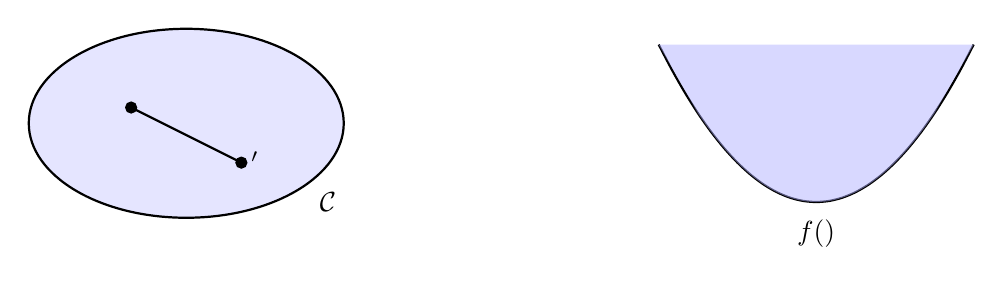
\begin{tikzpicture}
				\fill[blue!20, opacity=0.5] (-3,0) ellipse (2 and 1.2); 
				\draw[thick] (-3,0) ellipse (2 and 1.2);
				\filldraw[black] (-3.7,0.2) circle (2pt) node[left] {$\vw$};
				\filldraw[black] (-2.3,-0.5) circle (2pt) node[right] {$\vw'$};
				\draw[thick] (-3.7,0.2) -- (-2.3,-0.5);
				\node at (-1.2,-1.0) {$\mathcal{C}$};
				\begin{scope}[shift={(5,-1)}]
					\draw[thick, domain=-2:2, smooth, variable=\x] 
					plot ({\x}, {0.5*\x*\x});
					\fill[blue!30, opacity=0.5] 
					plot[domain=-1.5:1.5, smooth] ({\x}, {0.5*\x*\x}) -- 
					(2, {0.5*2*2}) -- 
					(-2, {0.5*2*2}) -- 
					cycle;
					\node at (0,-0.4) {$f(\weights)$};
				\end{scope}
			\end{tikzpicture}
			\vspace*{-8mm}
			\end{center}
			\caption{Left: A convex set $\cluster \subseteq \mathbb{R}^{\dimlocalmodel}$. 
				Right: A convex \gls{function} $f: \mathbb{R}^{\dimlocalmodel} \rightarrow \mathbb{R}$.
				\label{fig_convex_set_function_dict}}
		\end{figure}
		See also: \gls{euclidspace}, \gls{function}, \gls{epigraph}.},
	first={convex},
	text={convex}
}


\newglossaryentry{smooth}
{name={smooth},
	description={A\index{smooth} real-valued \gls{function} $f: \mathbb{R}^{\dimlocalmodel} \rightarrow \mathbb{R}$ 
		is smooth if it is \gls{differentiable} and its \gls{gradient} $\nabla f(\weights)$ is continuous at all $\weights \in \mathbb{R}^{\dimlocalmodel}$  \cite{nesterov04}, \cite{CvxBubeck2015}. 
		A smooth \gls{function} $f$ is referred to as $\beta$-smooth if the \gls{gradient} 
		$\nabla f(\weights)$ is Lipschitz continuous with Lipschitz constant $\beta$, i.e., 
		$$\| \nabla f(\weights) - \nabla f(\weights') \| \leq \beta \| \weights - \weights' \| \mbox{, for any } \weights,\weights' \in \mathbb{R}^{\dimlocalmodel}.$$ 
		The constant $\beta$ quantifies the amount of smoothness of the \gls{function} $f$: the smaller the $\beta$, 
		the smoother $f$ is. \Glspl{optproblem} with a smooth \gls{objfunc} can be solved effectively by \gls{gdmethods}. 
	    Indeed, \gls{gdmethods} approximate the \gls{objfunc} locally around a current choice $\weights$ 
	    using its \gls{gradient}. This approximation works well if the \gls{gradient} does 
	    not change too rapidly. We can make this informal claim precise by studying the effect of a single 
	    \gls{gradstep} with \gls{stepsize} $\lrate=1/\beta$ (see Figure \ref{fig_gd_smooth_dict}). 
	    \begin{figure}[H] 
	    	\begin{center} 
	    	\begin{tikzpicture}[scale=0.8, x=0.6cm,y=0.05cm]
	    		% Parameter to shift the quadratic curve horizontally
	    		\def\hshift{0.5} % Change this value to shift the curve horizontally
	    		% Define the function (only the increasing part of x^2 for x >= 0)
	    		\draw[thick, dashed, domain=\hshift:8+\hshift, smooth, variable=\x] plot ({\x}, {\x^2}); %node[right] {$f(x) = x^2$};
	    		% Define points for the tangents
	    		\coordinate (w) at (\hshift,{\hshift*\hshift}); % Point w on the curve (left end of the plot)
	    		\coordinate (wkplus1) at (4+\hshift,{(4+\hshift)^2}); % Point w^{k+1} on the curve (x=1 + hshift, y=1)
	    		\coordinate (wk) at (8+\hshift,{(8+\hshift)^2}); % Point w^k on the curve (right end of the plot)
	    		% Calculate the slopes for the tangents
  				\draw[line width=1pt, transform canvas={yshift=-1pt}] (wk) -- +(-2, -{4*(8 + \hshift)} ) -- +(1, {2*(8 + \hshift)}); % Tangent at w^k with positive slope
 				\draw[line width=1pt, transform canvas={yshift=-1pt}] (w) -- +(-1, {-{2*\hshift}} ) -- +(1, {+{2*\hshift}})  node[below] {$\nabla f(\weights)$};% Tangent at w with slope 0 (since derivative at hshift = 0)
%	    		% Draw filled circles at points w^k, w, and w^{k+1}
	    		\filldraw (wk) circle (2pt) node[above left] {$\weights^{(\iteridx)}$} node[below right, xshift=-15pt,yshift=-15pt] {$\nabla f(\weights^{(\iteridx)})$} ;
	    		\filldraw (w) circle (2pt) node[above right] {$\weights$} ;
	    		\filldraw (wkplus1) circle (2pt) node[below right] {$\weights^{(\iteridx+1)}\!=\!\weights^{(\iteridx)}\!-\!(1/\beta)\nabla f(\weights^{(\iteridx)})$};
	    		    % Draw horizontal rulers to mark the function values at wk and wk_plus1
	    		\draw[dashed] (wk) -- ($(8,0) + (wk)$) ; %node[left] {$f(\weights^{(\iteridx)})$};
	    		\draw[dashed] (wkplus1) -- ($(12,0) + (wkplus1)$) ; %node[left] {$f(\weights^{(\iteridx+1)})$};
	    		 \draw[<->, thick] ($(4,0) + (wk)$) -- ($(8,0) + (wkplus1)$) 
	    		node[midway, right] {$ f\big(\weights^{(\iteridx)}\big)\!-\!f\big(\weights^{(\iteridx+1)}\big)\!\geq\!\frac{1}{2\beta}\normgeneric{\nabla f(\weights^{(\iteridx)})}{2}^{2}$};
%	    		% Label the curve
%	    		\node at (2, 4) {};
	    	\end{tikzpicture}
	    	\end{center}
	    	\caption{Consider an \gls{objfunc} $f(\weights)$ that is $\beta$-smooth. 
	    		Taking a \gls{gradstep}, with \gls{stepsize} $\lrate = 1/\beta$, decreases the 
	    		objective by at least $\frac{1}{2\beta}\normgeneric{\nabla f(\weights^{(\iteridx)})}{2}^{2}$ \cite{nesterov04}, \cite{CvxBubeck2015}, \cite{CvxAlgBertsekas}. 
	    		Note that the \gls{stepsize} $\lrate = 1/\beta$ becomes larger for smaller $\beta$. Thus, 
	    		for smoother \glspl{objfunc} (i.e., those with smaller $\beta$), 
				we can take larger steps. \label{fig_gd_smooth_dict}}
	    	\end{figure}
		See also: \gls{function}, \gls{differentiable}, \gls{gradient}, \gls{optproblem}, \gls{objfunc}, \gls{gdmethods}, \gls{gradstep}, \gls{stepsize}.},
	first={smooth},
	text={smooth}
}

\newglossaryentry{paramspace}
{name={parameter space},
	description={The\index{parameter space} \gls{parameter} space $\paramspace$ of 
		an \gls{ml} \gls{model} $\hypospace$ is the set of all feasible choices for the 
		\gls{modelparams} (see Figure \ref{fig_param_space_dict}). Many important \gls{ml} methods 
		use a \gls{model} that is parametrized by vectors of the \gls{euclidspace} $\mathbb{R}^{\dimlocalmodel}$. 
		Two widely used examples of parametrized \glspl{model} are \glspl{linmodel} 
		and \glspl{deepnet}. The \gls{parameter} space is then often a subset $\paramspace \subseteq \mathbb{R}^{\dimlocalmodel}$, 
		e.g., all vectors $\weights \in \mathbb{R}^{\dimlocalmodel}$ with a \gls{norm} smaller than one.
		\begin{figure}[H]
			\begin{center}
			\begin{tikzpicture}
				% Left part: Ellipse representing parameter space (with two dots)
				\node[ellipse, minimum width=3cm, minimum height=2cm, draw, thick] (paramspace) {};
				\node[below=0.1cm of paramspace] {\gls{parameter} space $\paramspace$};
				% Two dots inside the left ellipse
				\node[black, circle, inner sep=2pt, fill] (theta1) at ($(paramspace.north west) + (1, -1)$) {};
				\node[left=0.01cm of theta1] {$\weights$};
				\node[black, circle, inner sep=2pt, fill] (theta2) at ($(paramspace.south east) + (-1.5, 1)$) {};
				\node[left=0.01cm of theta2] {$\weights'$};
				% Right part: Ellipse containing two smaller plots
				\node[ellipse, minimum width=7cm, minimum height=3cm, draw, thick, right=4cm of paramspace] (plotcloud) {};
				\node[above=0.2cm of plotcloud] {\gls{model} $\hypospace$};
				% Axis for first smaller plot
				\node (plot1start) at ($(plotcloud.south west) + (0.2, 0.2)$) {};
				%\draw[thick, ->] (plot1start) -- ++(2, 0) node[anchor=north] {$\featurevec$};
				%\draw[thick, ->] (plot1start) -- ++(0, 1.5) node[anchor=east] {$\truelabel$};
				% Simple plot line in first smaller plot
				\draw[thick, red] (plot1start) .. controls ++(0.8, 1) and ++(-0.8, -0.8) .. ($(plotcloud.south west) + (2.8, 0.8)$) node[anchor=west] {$\hypothesis^{(\weights)}$};
				% Axis for second smaller plot
				\node (plot2start) at ($(plotcloud.south west) + (1.0, 1.2)$) {};
			%	\draw[thick, ->] (plot2start) -- ++(2, 0) node[anchor=north] {$\featurevec$};
			%	\draw[thick, ->] (plot2start) -- ++(0, 1.5) node[anchor=east] {$\truelabel$};
				% Simple plot line in second smaller plot
				\draw[thick, blue] (plot2start) .. controls ++(0.8, 0.5) and ++(-0.8, -0.8) .. ($(plotcloud.south west) + (2.8, 2.1)$) node[anchor=west] {$\hypothesis^{(\weights')}$};
				% Connect the two dots in the parameter space to the two plots
				\draw[thick, ->, bend right=20] (theta1) to ($(plot1start) + (0,0)$);
				\draw[thick, ->, bend left=20] (theta2) to (plot2start);
			\end{tikzpicture}
			\end{center} 
			\caption{The \gls{parameter} space $\paramspace$ of an \gls{ml} \gls{model} $\hypospace$ consists of all 
			feasible choices for the \gls{modelparams}. Each choice $\weights$ for the \gls{modelparams} 
			selects a \gls{hypothesis} \gls{map} $\hypothesis^{(\weights)} \in \hypospace$.
				 \label{fig_param_space_dict}} 
\end{figure}
		See also: \gls{parameter}, \gls{model}, \gls{modelparams}.},
	first={parameter space},
	text={parameter space}
}

\newglossaryentry{datanorm}
{name={data normalization},
	description={\Gls{data} normalization\index{data normalization} refers to transformations 
		applied to the \glspl{featurevec} of \glspl{datapoint} to improve the \gls{ml} method's 
		\gls{statasp} or \gls{compasp}. For example, in \gls{linreg} with \gls{gdmethods} using 
		a fixed \gls{learnrate}, convergence depends on controlling the \gls{norm} of \glspl{featurevec} 
		in the \gls{trainset}. A common approach is to normalize \glspl{featurevec} such that their 
		\gls{norm} does not exceed one \cite[Ch.\ 5]{MLBasics}.
				\\
		See also: \gls{data}, \gls{featurevec}, \gls{datapoint}, \gls{ml}, \gls{statasp}, \gls{compasp}, \gls{linreg}, \gls{gdmethods}, \gls{learnrate}, \gls{norm}, \gls{trainset}.},
	first={data normalization},
	text={data normalization}
}

\newglossaryentry{dataaug}
{name={data augmentation},
	description={\Gls{data} augmentation\index{data augmentation} methods add synthetic \glspl{datapoint} 
		to an existing set of \glspl{datapoint}. These synthetic \glspl{datapoint} are obtained by 
		perturbations (e.g., adding noise to physical measurements) or transformations 
		(e.g., rotations of images) of the original \glspl{datapoint}. These perturbations and 
		transformations are such that the resulting synthetic \glspl{datapoint} should 
		still have the same \gls{label}. As a case in point, a rotated cat image is still 
		a cat image even if their \glspl{featurevec} (obtained by stacking pixel color intensities) 
		are very different (see Figure \ref{fig_symmetry_dataaug_dict}). \Gls{data} augmentation can be an 
		efficient form of \gls{regularization}.
		\begin{figure}[H]
		\begin{center}
			\begin{tikzpicture}
				% Define shift macros locally
				\newcommand{\xshift}{0.5}
				\newcommand{\yshift}{2}
				% Define the shifted curves
				% Define the shifted curves
  				\draw[very thick, blue] plot[smooth, tension=1] coordinates {(0,0) (2,1) (4,0) (6,-1) (8,0)};
  				\node[blue, right] at (0,0) {\textbf{cat}};
  				\draw[very thick, red, dashed] plot[smooth, tension=1] coordinates {(0 + \xshift,0 + \yshift) (2 + \xshift,1 + \yshift) (4 + \xshift,0 + \yshift) (6 + \xshift,-1 + \yshift) (8 + \xshift,0 + \yshift)};
  				\node[red, right] at (8 + \xshift,0 + \yshift) {\textbf{no cat}};
				\fill[blue] (2,1) circle (2pt) node[above] {$\featurevec^{(1)}$};
				\fill[blue] (6,-1) circle (2pt) node[above] {$\featurevec^{(2)}$};
				  % Draw a bent arrow connecting the two points with custom in and out angles
				  \draw[->, thin, >=latex, line width=0.5pt] (2,1) to[out=240, in=240] node[midway, below] {$\mathcal{T}^{(\eta)}$} (6,-1);
			  \end{tikzpicture}
			  \vspace*{-11mm}
		\end{center}
		\caption{\Gls{data} augmentation exploits intrinsic symmetries of \glspl{datapoint} in 
		       some \gls{featurespace} $\featurespace$. We can represent a symmetry by 
		     an operator $\mathcal{T}^{(\eta)}: \featurespace \rightarrow \featurespace$,
		     parametrized by some number $\eta \in \mathbb{R}$. For example, $\mathcal{T}^{(\eta)}$ 
		    might represent the effect of rotating a cat image by $\eta$ degrees. A \gls{datapoint} 
		    with \gls{featurevec} $\featurevec^{(2)} = \mathcal{T}^{(\eta)} \big(\featurevec^{(1)} \big)$ must 
		    have the same \gls{label} $\truelabel^{(2)}=\truelabel^{(1)}$ as a \gls{datapoint} 
		     with \gls{featurevec} $\featurevec^{(1)}$.\label{fig_symmetry_dataaug_dict}}
		 \end{figure}
		See also: \gls{data}, \gls{datapoint}, \gls{label}, \gls{featurevec}, \gls{regularization}, \gls{featurespace}. },
	first={data augmentation},
	text={data augmentation}
}
	
	
\newglossaryentry{localdataset}
{name={local dataset}, plural={local datasets}, 
	description={The\index{local dataset} concept of a local \gls{dataset} is 
		in between the concept of a \gls{datapoint} and a \gls{dataset}. A local \gls{dataset} consists of several 
		individual \glspl{datapoint}, which are characterized by \glspl{feature} and \glspl{label}. 
		In contrast to a single \gls{dataset} used in basic \gls{ml} methods, a local \gls{dataset} is also 
		related to other local \glspl{dataset} via different notions of similarity. These similarities 
		might arise from \glspl{probmodel} or communication infrastructure and 
		are encoded in the edges of an \gls{empgraph}.
				\\
		See also: \gls{dataset}, \gls{datapoint}, \gls{feature}, \gls{label}, \gls{ml}, \gls{probmodel}, \gls{empgraph}.},
		first={local dataset},
		text={local dataset}
}
	
\newglossaryentry{localmodel}
{name={local model}, plural={local models}, 
	description={Consider\index{local model} a collection of \glspl{device} that are represented 
		as nodes $\nodes$ of an \gls{empgraph}. A local \gls{model} $\localmodel{\nodeidx}$ 
		is a \gls{hypospace} assigned to a node $\nodeidx \in \nodes$. Different nodes might be 
		assigned different \glspl{hypospace}, i.e., in general $\localmodel{\nodeidx} \neq \localmodel{\nodeidx'}$ for different 
		nodes $\nodeidx, \nodeidx' \in \nodes$. 
				\\
		See also: \gls{device}, \gls{empgraph}, \gls{model}, \gls{hypospace}. },
	first={local model},
	text={local model}
}
	
\newglossaryentry{mutualinformation}
{name={mutual information (MI)},
 	description={The\index{mutual information (MI)} MI $\mutualinformation{\featurevec}{\truelabel}$ 
 		between two \glspl{rv} $\featurevec$, $\truelabel$ defined on the same \gls{probspace} 
 		is given by \cite{coverthomas} $$\mutualinformation{\featurevec}{\truelabel} \defeq 
		\expect \left\{ \log \frac{p (\featurevec,\truelabel)}{p(\featurevec)p(\truelabel)} \right\}.$$ 
		It is a measure of how well we can estimate $\truelabel$ based 
		solely on $\featurevec$. A large value of $\mutualinformation{\featurevec}{\truelabel}$ indicates that 
		$\truelabel$ can be well predicted solely from $\featurevec$. This \gls{prediction} could be obtained by a 
		\gls{hypothesis} learned by an \gls{erm}-based \gls{ml} method. 
				\\
		See also: \gls{rv}, \gls{probspace}, \gls{prediction}, \gls{hypothesis}, \gls{erm}, \gls{ml}. }, 
	first={MI}, 
	text={MI} 
}

\newglossaryentry{zerogradientcondition}
{name={zero-gradient condition},
	description={Consider\index{zero-gradient condition} the unconstrained 
		\gls{optproblem} $\min_{\weights \in \mathbb{R}^{\dimlocalmodel}} f(\weights)$  with 
			a \gls{smooth} and \gls{convex} \gls{objfunc} $f(\weights)$. A necessary and 
			sufficient condition for a vector $\widehat{\weights} \in \mathbb{R}^{\dimlocalmodel}$ 
			to solve this problem is that the \gls{gradient} $\nabla f \big( \widehat{\weights} \big)$ 
			is the zero vector such that
			$$ \nabla f \big( \widehat{\weights} \big) = \mathbf{0} \Leftrightarrow  f \big( \widehat{\weights} \big) = \min_{\weights \in \mathbb{R}^{\dimlocalmodel}} f(\weights) .$$ 
					\\
			See also: \gls{optproblem}, \gls{smooth}, \gls{convex}, \gls{objfunc}, \gls{gradient}.}, 
		first={zero-gradient condition},
		text={zero-gradient condition}
}


\newglossaryentry{edgeweight}
{name={edge weight},
	description={Each\index{edge weight} edge $\edge{\nodeidx}{\nodeidx'}$ of an \gls{empgraph} is 
		assigned a non-negative edge weight $\edgeweight_{\nodeidx,\nodeidx'}\geq0$. 
		A zero edge weight $\edgeweight_{\nodeidx,\nodeidx'}=0$ indicates the absence 
		of an edge between nodes $\nodeidx, \nodeidx' \in \nodes$.
				\\
		See also: \gls{empgraph}.}, 
	first={edge weight},
	text={edge weight}
}


\newglossaryentry{dataminprinc}
{name={data minimization principle},
	description={European\index{data minimization principle} \gls{data} protection regulation 
		includes a \gls{data} minimization principle. This principle requires a \gls{data} controller to 
		limit the collection of personal information to what is directly relevant and necessary 
		to accomplish a specified purpose. The \gls{data} should be retained only for as long as 
		necessary to fulfill that purpose \cite[Article 5(1)(c)]{GDPR2016}, \cite{EURegulation2018}.
				\\
		See also: \gls{data}.}, 
	first={data minimization principle},
	text={data minimization principle}
}


